\documentclass[acmtog]{acmart}
\usepackage{lipsum}
\usepackage{physics}

\usepackage{caption}
\usepackage{subcaption}

\usepackage{graphicx}
\usepackage{xcolor}

\newcommand{\draft}[1]{\noindent\textcolor{red}{\texttt{#1}}}

\setcopyright{none} 
\makeatletter
\let\@authorsaddresses\@empty
\makeatother
\settopmatter{printacmref=false}
\renewcommand\footnotetextcopyrightpermission[1]{}
\AtBeginDocument{%
  \providecommand\BibTeX{{%
    Bib\TeX}}}
\begin{document}

\title{CompSim hand-in week 3}
\author{Carl Ivarsen Askehave}
\affiliation{
  \institution{(wfq585)}
  \country{University of Copenhagen}
}

\maketitle
\thispagestyle{empty}

\section{Introduction}
In this report we'll look at different common quality measures for trianglur
and tetrahedral meshes. We'll also look at, and implement, a simple
computational mesh generator called the \emph{marching triangles algorithm}.
Afterwards we're going to generate a couple of meshes using our implemented
algortihm and also using the 3rd party sotware called Wildmeshing. Finally
we'll compare the quality of the meshes generated by the two different methods
using the quality measures we've looked at.

\subsection*{What is a mesh?}
A mesh is a discretization of a continuous domain into a finite number of
elements. The elements are usually simple shapes like triangles (2D) or
tetrahedra (3D), which are easy to work with computationally. The mesh is used
to approximate the continuous domain, with the purpose to solve partial
differential equations numerically. The quality of the mesh can greatly impact
the accuracy of the solution.

\section{Mesh quality measures}
All meshes aren't created equal, in the sense that the elements used to
generate the mesh, can have different shapes, which can greatly impact the
performance of the mesh in simulation. Therefore it is important to have a way
to measure the quality of the mesh. Usually the quality of the mesh is related
to the \textit{regularity} of the subshapes, which is a measure of how close
the subshape is to a regular shape, like an equilateral triangle or a regular
tetrahedron. The regularity of the shapes can be captured with a couple of
different measures, which we will look at in this section.

\subsection*{Radius ratio}
One way to measure the quality of a subshape is to look at it's radius ratio,
which is the ratio between the radius of the inscribed circle $r_\mathrm{in}$
and the radius of the circumscribed circle $r_\mathrm{circ}$. This quality
measure can be expressed in the following way for triangles and tetrahedra
%
\begin{align}
  Q_R^\mathrm{tri} & = 2 \, \frac{r_\mathrm{in}}{r_\mathrm{circ}}, \\
  Q_R^\mathrm{tet} & = 3 \, \frac{r_\mathrm{in}}{r_\mathrm{circ}},
\end{align}
%
where the coefficients in front are decided by the dimensionality of the shape.
These are both \textit{fair measures}, meaning that they approach the value 1
for regular shapes.

\subsection*{Volume ratio}
Another way to probe the quality of a shape is to compare it's volume to the
volume of an ideal, regular shape of the same size. For triangles we'd of
course have to compare the areas. This quality measure can be expressed in the
following way for triangles and tetrahedra
%
\begin{align}
  Q_V^\mathrm{tri} & = \frac{4}{\sqrt{3}}\frac{A}{\ell_\mathrm{rms}^2}, \\
  Q_V^\mathrm{tet} & = 6 \sqrt{2} \frac{V}{\ell_\mathrm{rms}^3},
\end{align}
%
where the \textit{root mean square length} is defined as $\ell_\mathrm{rms} =
  \sqrt{(\sum_i^N \ell_i^2)/N} $. When we have a quality measure for each
subshape in the mesh, we can iterate over all the shapes in a mesh and keep
track of all their individual quality measures, and plot them in a histogram.
This way we can get a sense of the overall quality of the mesh.

\begin{figure}
  \centering
  \begin{subfigure}{0.22\textwidth}
    \centering
    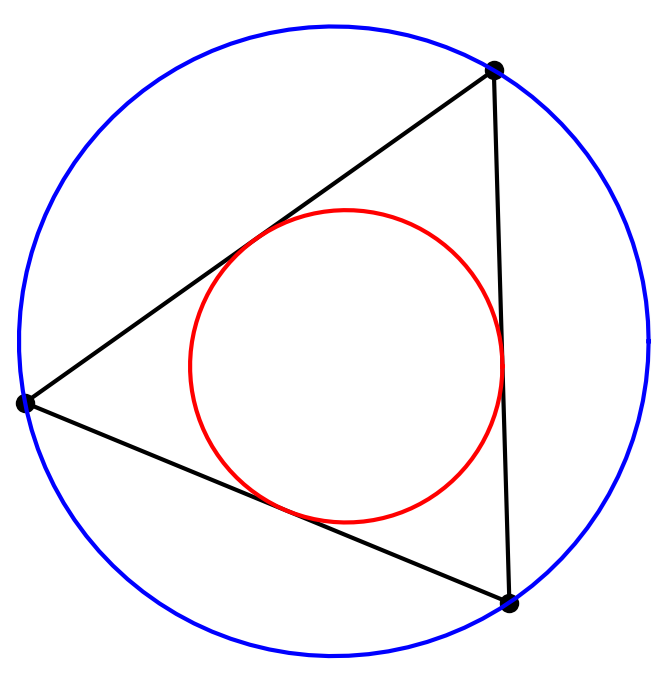
\includegraphics[width=\textwidth]{Images/triangle_regular.png}
  \end{subfigure}
  \begin{subfigure}{0.22\textwidth}
    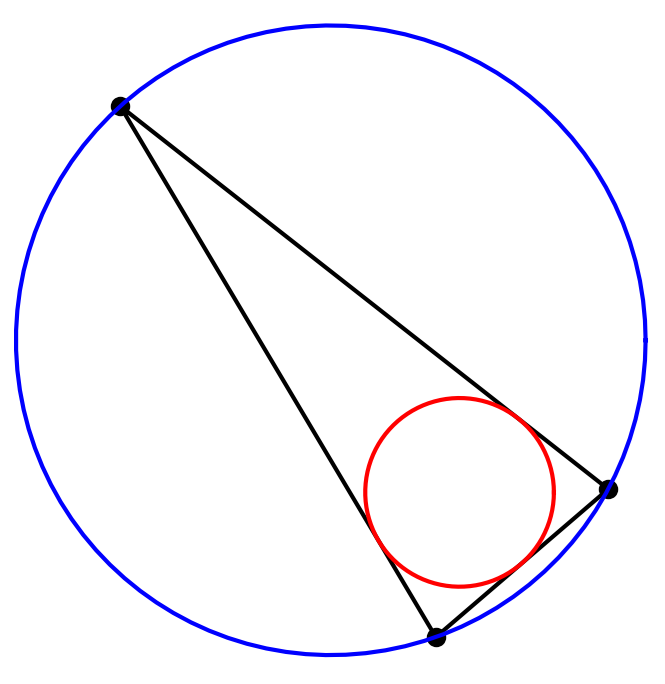
\includegraphics[width=\textwidth]{Images/triangle_iregular.png}
    \centering
  \end{subfigure}\hfill
  \caption{Illustrations of a regular (left) and an irregular (right) triangle along with their respective inscribed (red) and circumscribed (blue) circles. We see that for the regular triangle, the radii of the inscribed and circumscribed circles are closer than in the other case.}
\end{figure}

\section{The marching triangles algorithm}
The marching triangles algorithm is an algorithm for generating a 2D, planar
mesh bounded by an aribitrary polygon. The algorithm is implemented according
to the following steps:
%
\begin{itemize}
  \item Generate a square grid of evenly spaced points that completely covers the
        polygon.
  \item Compute the signed distance function (SDF) of the polygon for each point in the
        grid.
  \item For each square in the grid, generate 2 triangles that cover the square. All
        the triangles will have sides of lengths of 1, 1 and $\sqrt{2}$.
  \item For each triangle in the mesh, evaluate the SDF at the 3 vertices of the
        triangle, and handle the following cases:
        \begin{itemize}
          \item[Case 1:] If the SDF is negative in all three vertices, the triangle is inside
                the polygon and we keep the triangle.
          \item[Case 2:] If the SDF is positive in all three vertices, the triangle is outside
                the polygon and we discard the triangle.
          \item[Case 3:] If the SDF is negative in one vertex, we project the other two
                vertices onto the 0 contour of the SDF and keep the triangle.
          \item[Case 4:] If the SDF is negative in two vertices, we project the third vertex
                onto the 0 contour twice, first in the direction of the first vertex inside and
                second in the direction of the other vertex inside. We then keep the two
                triangles that are formed by the two projections and the two vertices inside.
        \end{itemize}
\end{itemize}

\begin{figure}[H]
  \centering
  \begin{subfigure}{0.22\textwidth}
    \centering
    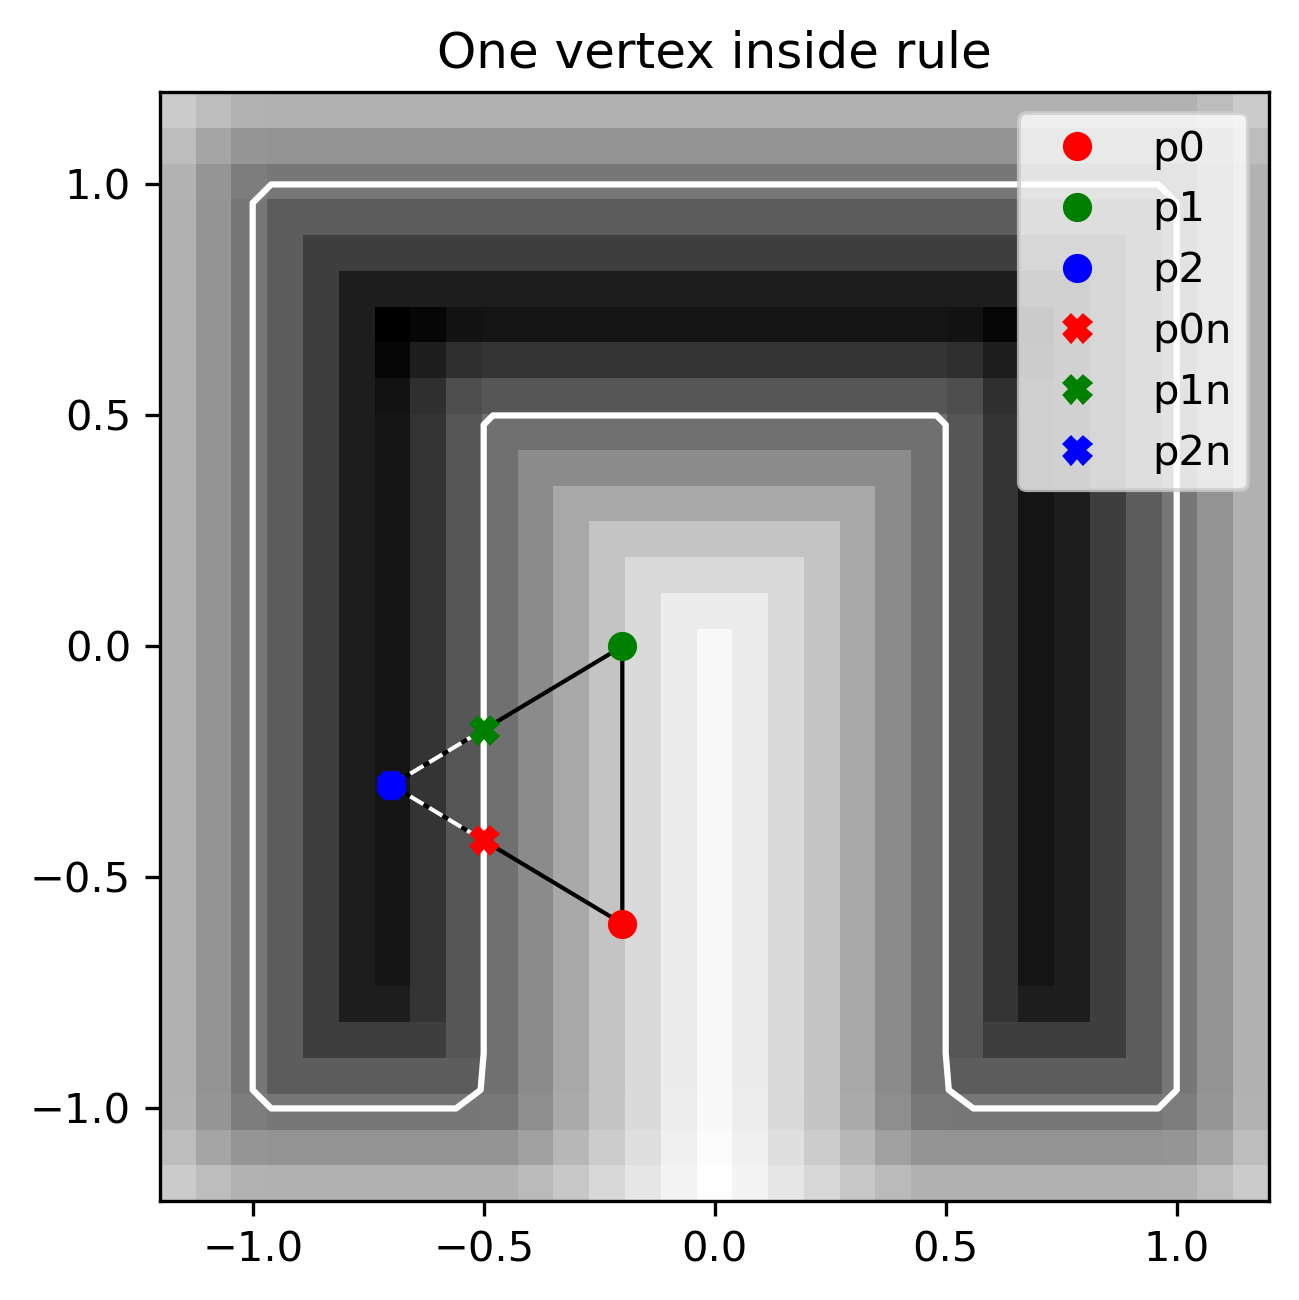
\includegraphics[width=\textwidth]{Images/one_inside_rule.png}
  \end{subfigure}
  \begin{subfigure}{0.22\textwidth}
    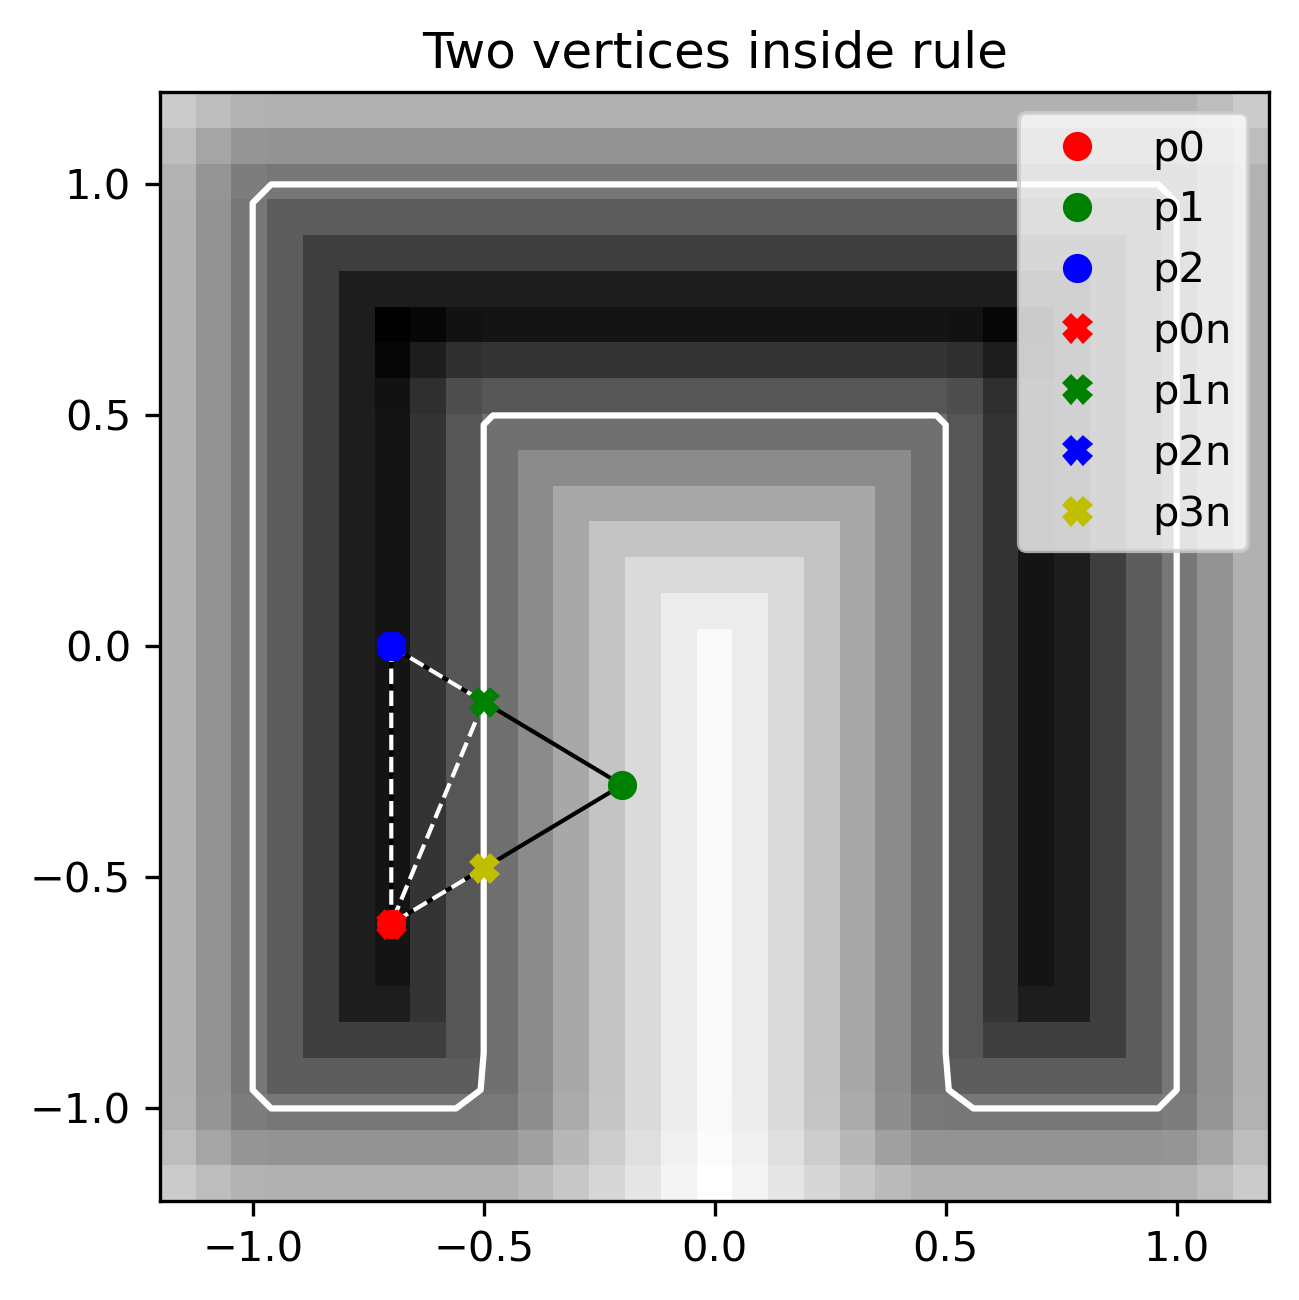
\includegraphics[width=\textwidth]{Images/two_inside_rule.png}
    \centering
  \end{subfigure}\hfill
  \caption{Illustrations of the rules applied for the two special cases in the algorithm. In the first one we have one vertex inside the polygon, and in the second we have two. We can see that in the first case we end up with one triangle, whereas in the second case we end up fabricating an aditional triangle.}
\end{figure}

\begin{figure}[H]
  \centering
  \begin{subfigure}{0.3\textwidth}
    \centering
    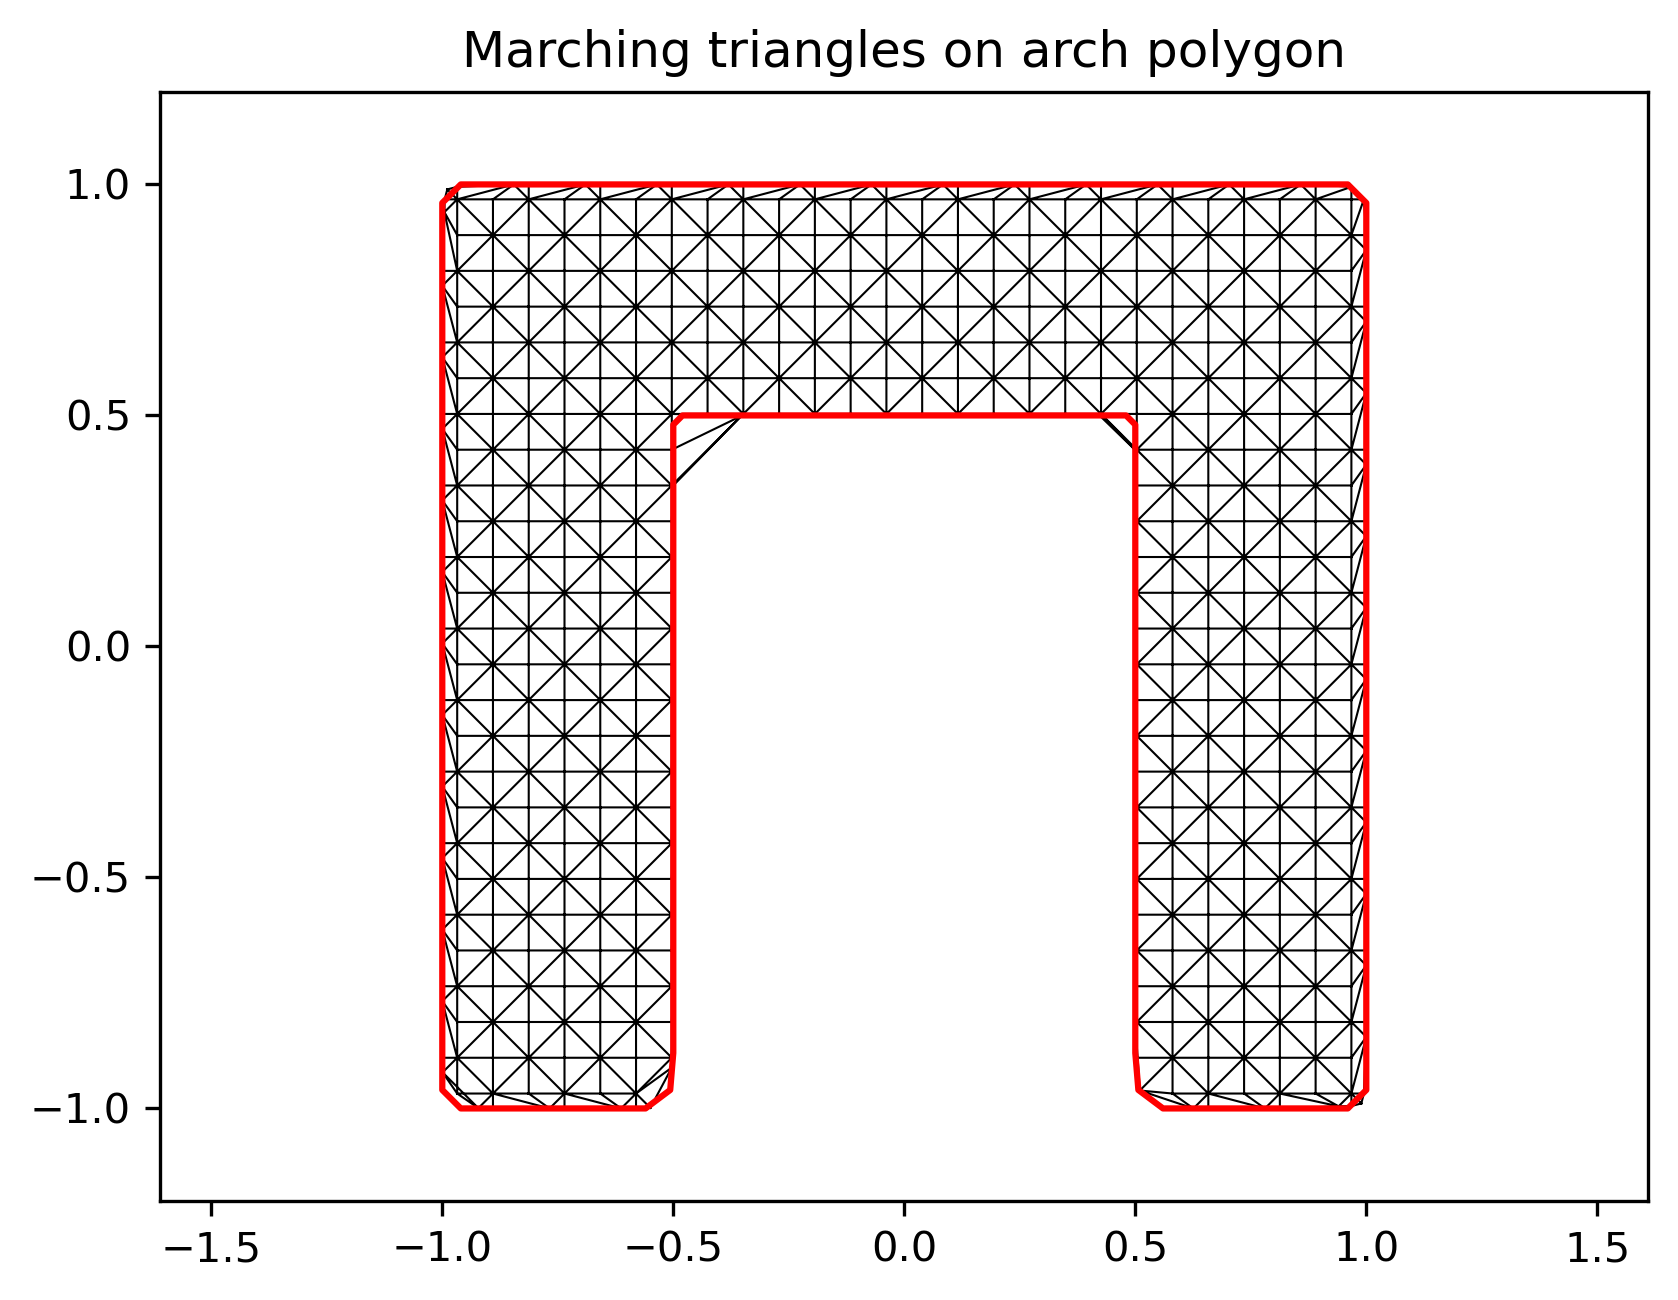
\includegraphics[width=\textwidth]{Images/marching_triangles_arch.png}
  \end{subfigure}
  \begin{subfigure}{0.3\textwidth}
    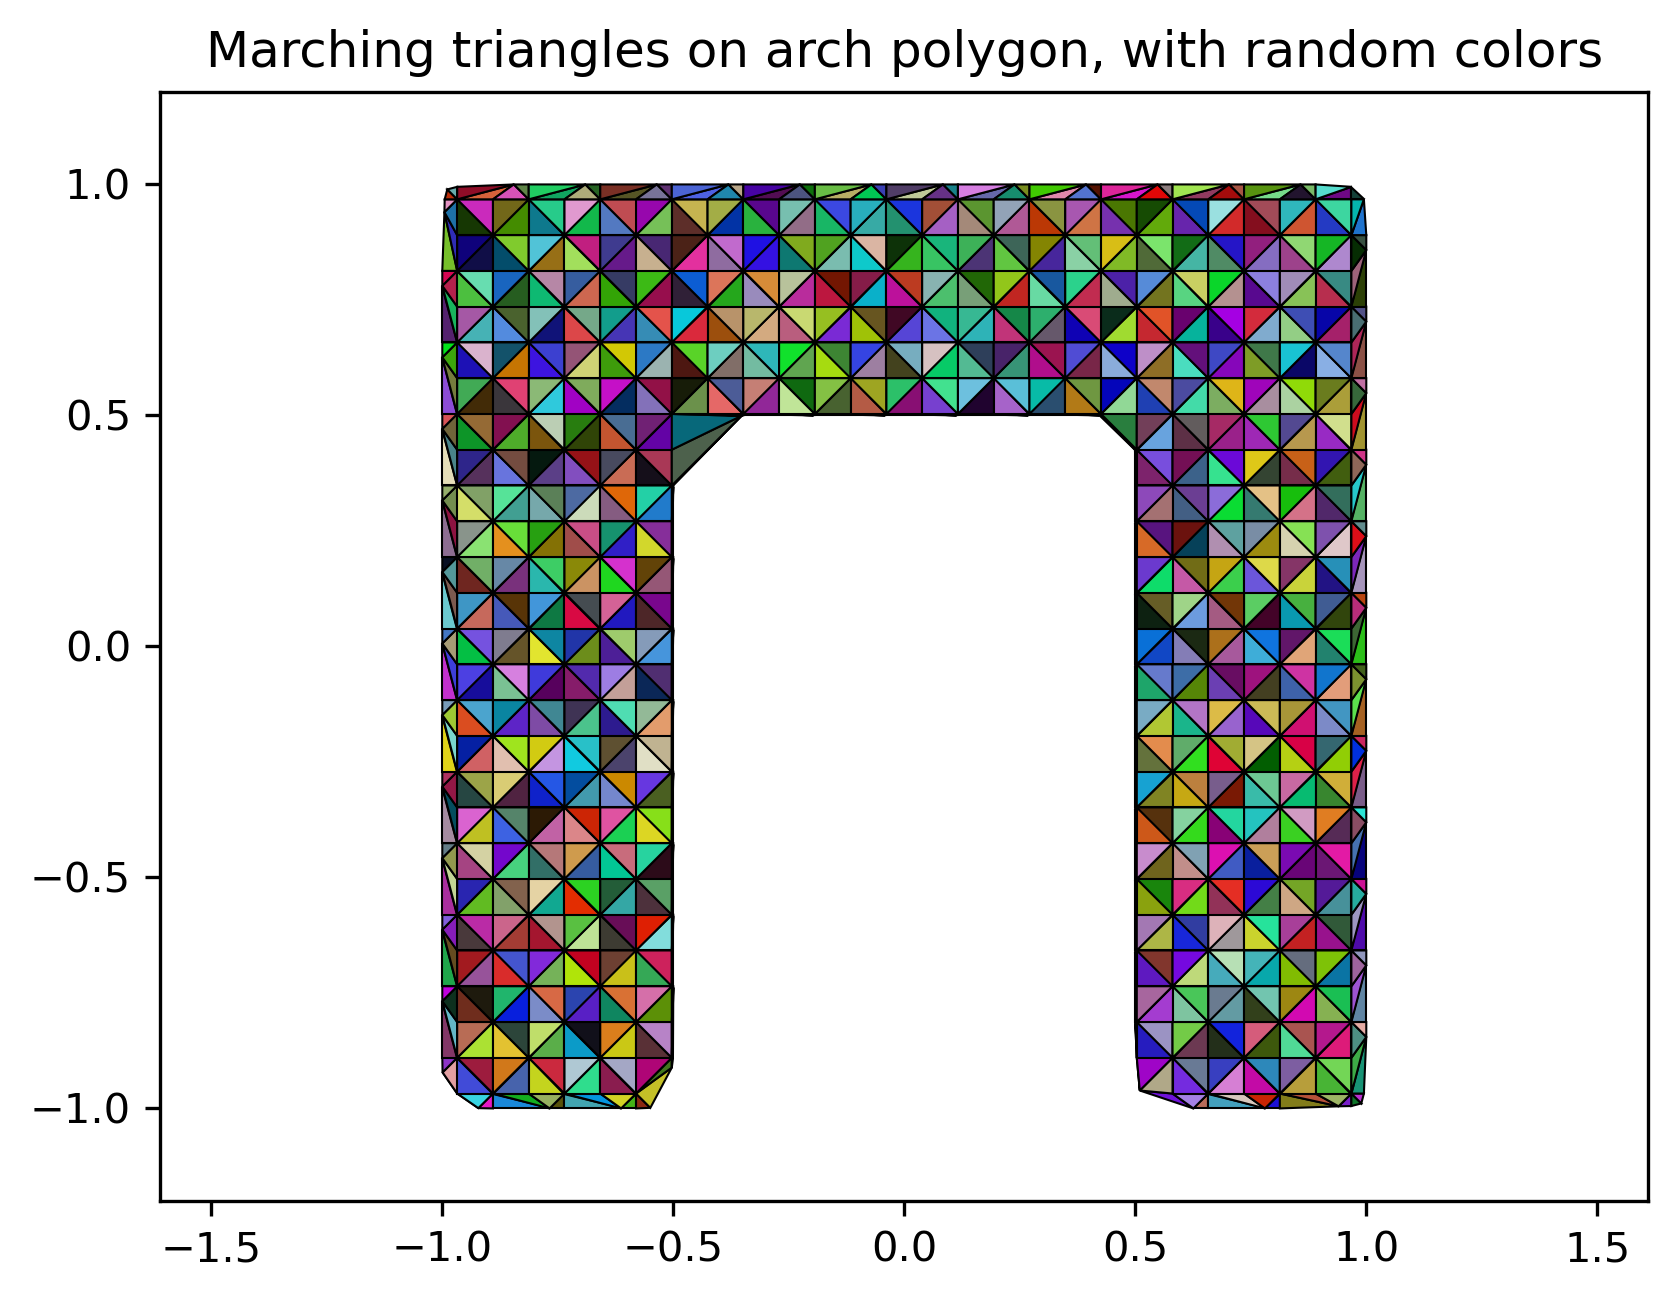
\includegraphics[width=\textwidth]{Images/marching_triangles_arch_colors.png}
    \centering
  \end{subfigure}\hfill
  \caption{The resluts of applying our marching triangles algorithm for the provided polygon. In the first image, we have plotted the contur of the SDF, to verify that our algorithm follows the boundary. We see that this is mostly the case except for a few inaccuracies, e.g. around the upper left corner on the inside. A problem with the first image is, that it's actually not clear whether we have correctly generated all the triangles in the mesh, since we can only see their edges. In the second image we have given each triangle a random color to verify that we actually did create them all, and we can see that we did.}
\end{figure}

\section{Generating meshes}
In this section we'll generate meshes for a couple of different shapes using
our own marching triangles algorithm and the algorithm from the Wildmeshing
library. Let's see how they both did.

\subsection*{Tetrahedral meshes}
\begin{figure}[H]
  \centering
  \begin{subfigure}{0.22\textwidth}
    \centering
    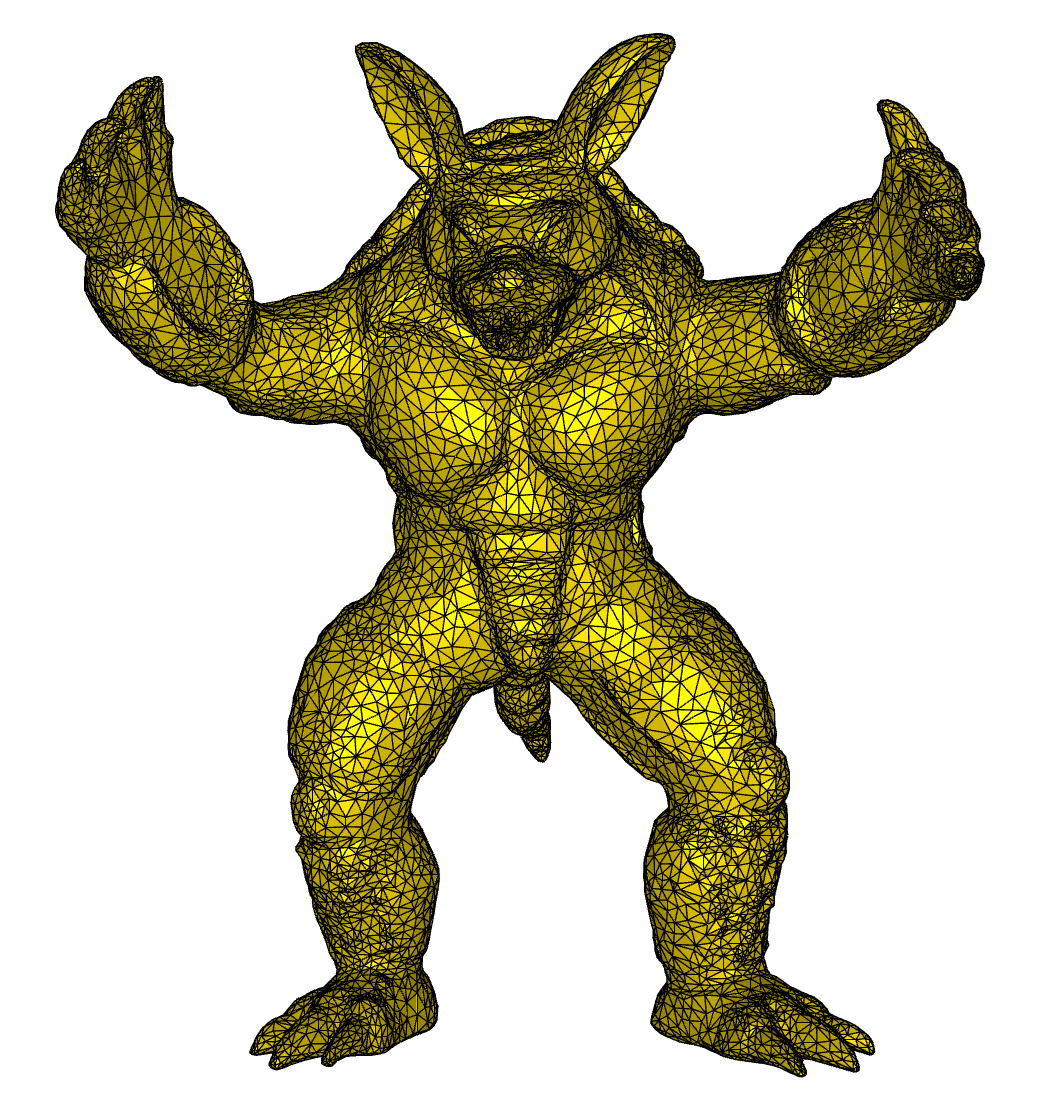
\includegraphics[width=\textwidth]{Images/armadillo_coarse.png}
  \end{subfigure}
  \begin{subfigure}{0.22\textwidth}
    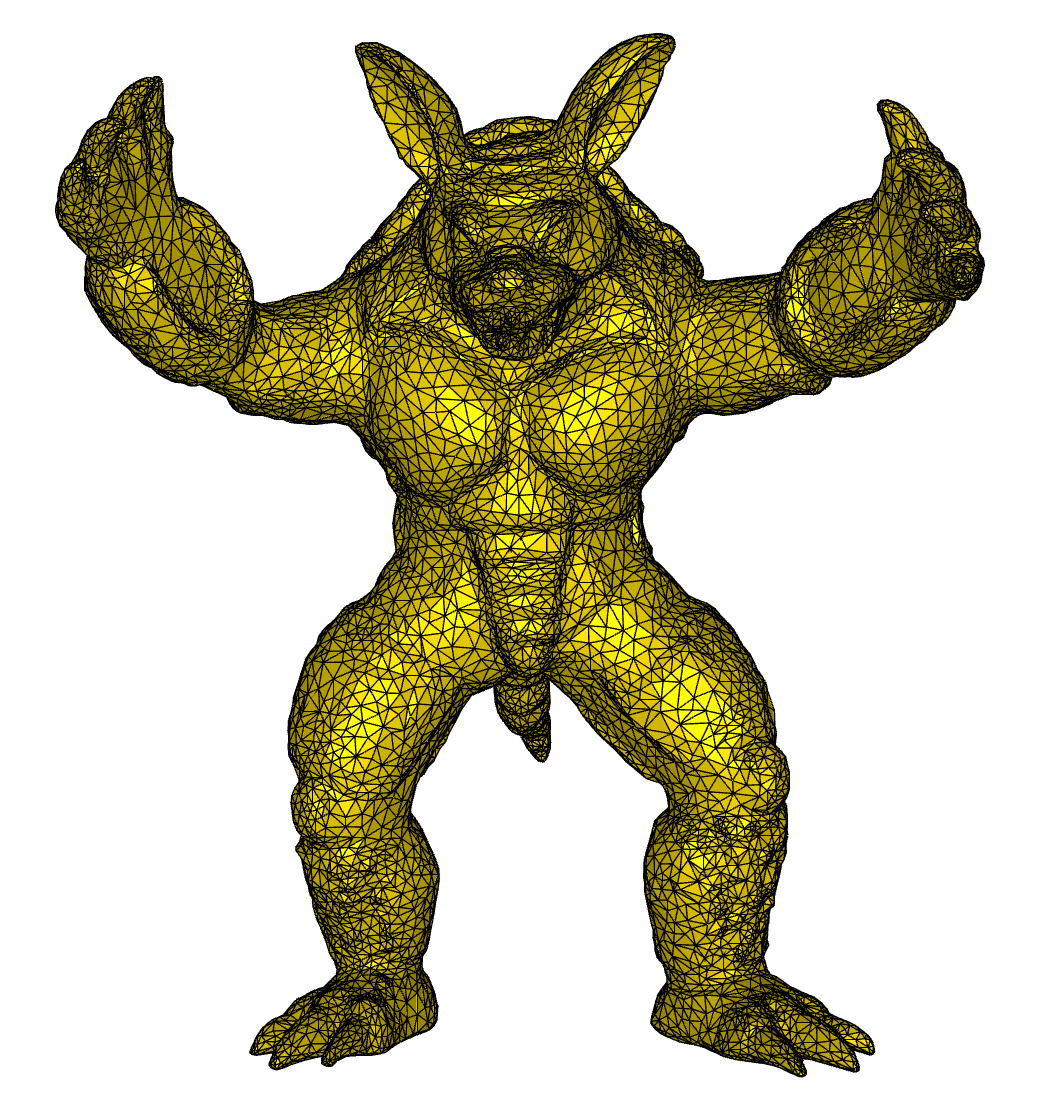
\includegraphics[width=\textwidth]{Images/armadillo_fine.png}
    \centering
  \end{subfigure}\hfill
  \caption{Result of the Wildmeshing tetrahedralizer on the armadillo model for edge length settings $l_\mathrm{edge}  = 0.05$ (left) and $l_\mathrm{edge}  = 0.0125$ (right).}
\end{figure}

\begin{figure}[H]
  \centering
  \begin{subfigure}{0.22\textwidth}
    \centering
    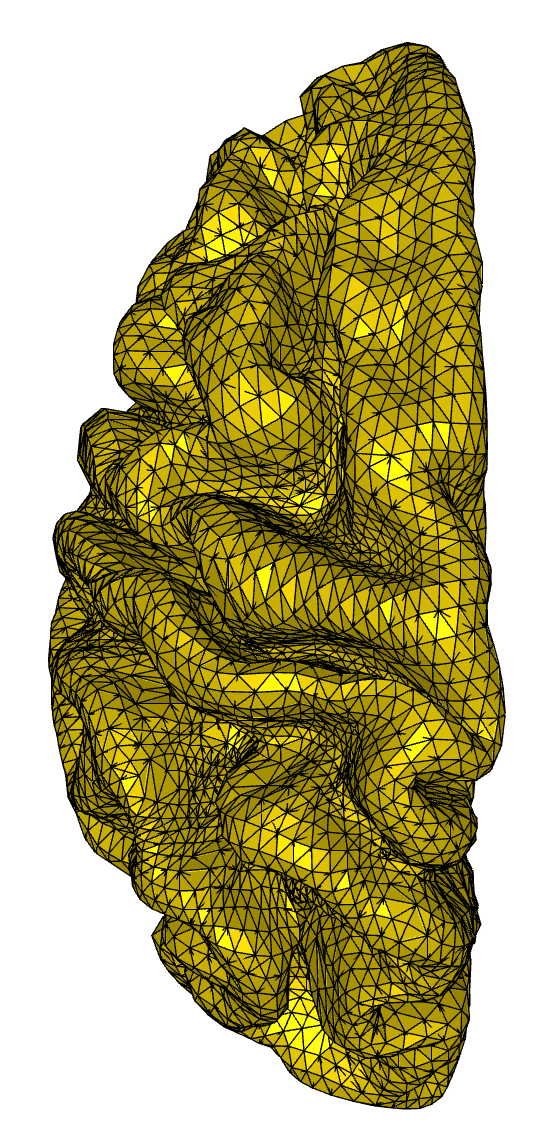
\includegraphics[width=\textwidth]{Images/left_brain_coarse.png}
  \end{subfigure}
  \begin{subfigure}{0.22\textwidth}
    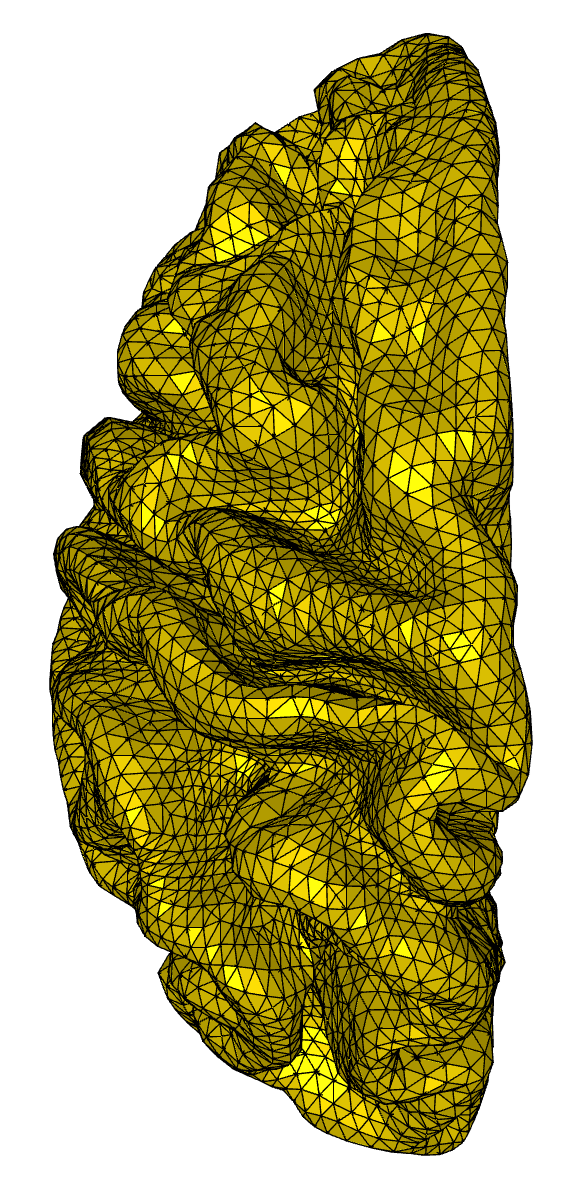
\includegraphics[width=\textwidth]{Images/left_brain_fine.png}
    \centering
  \end{subfigure}\hfill
  \caption{Result of the Wildmeshing tetrahedralizer on the left brain model for edge length settings $l_\mathrm{edge}  = 0.05$ (left) and $l_\mathrm{edge}  = 0.0125$ (right).}
\end{figure}

\subsection*{Triangular meshes}

\begin{figure}[H]
  \centering
  \begin{subfigure}{0.22\textwidth}
    \centering
    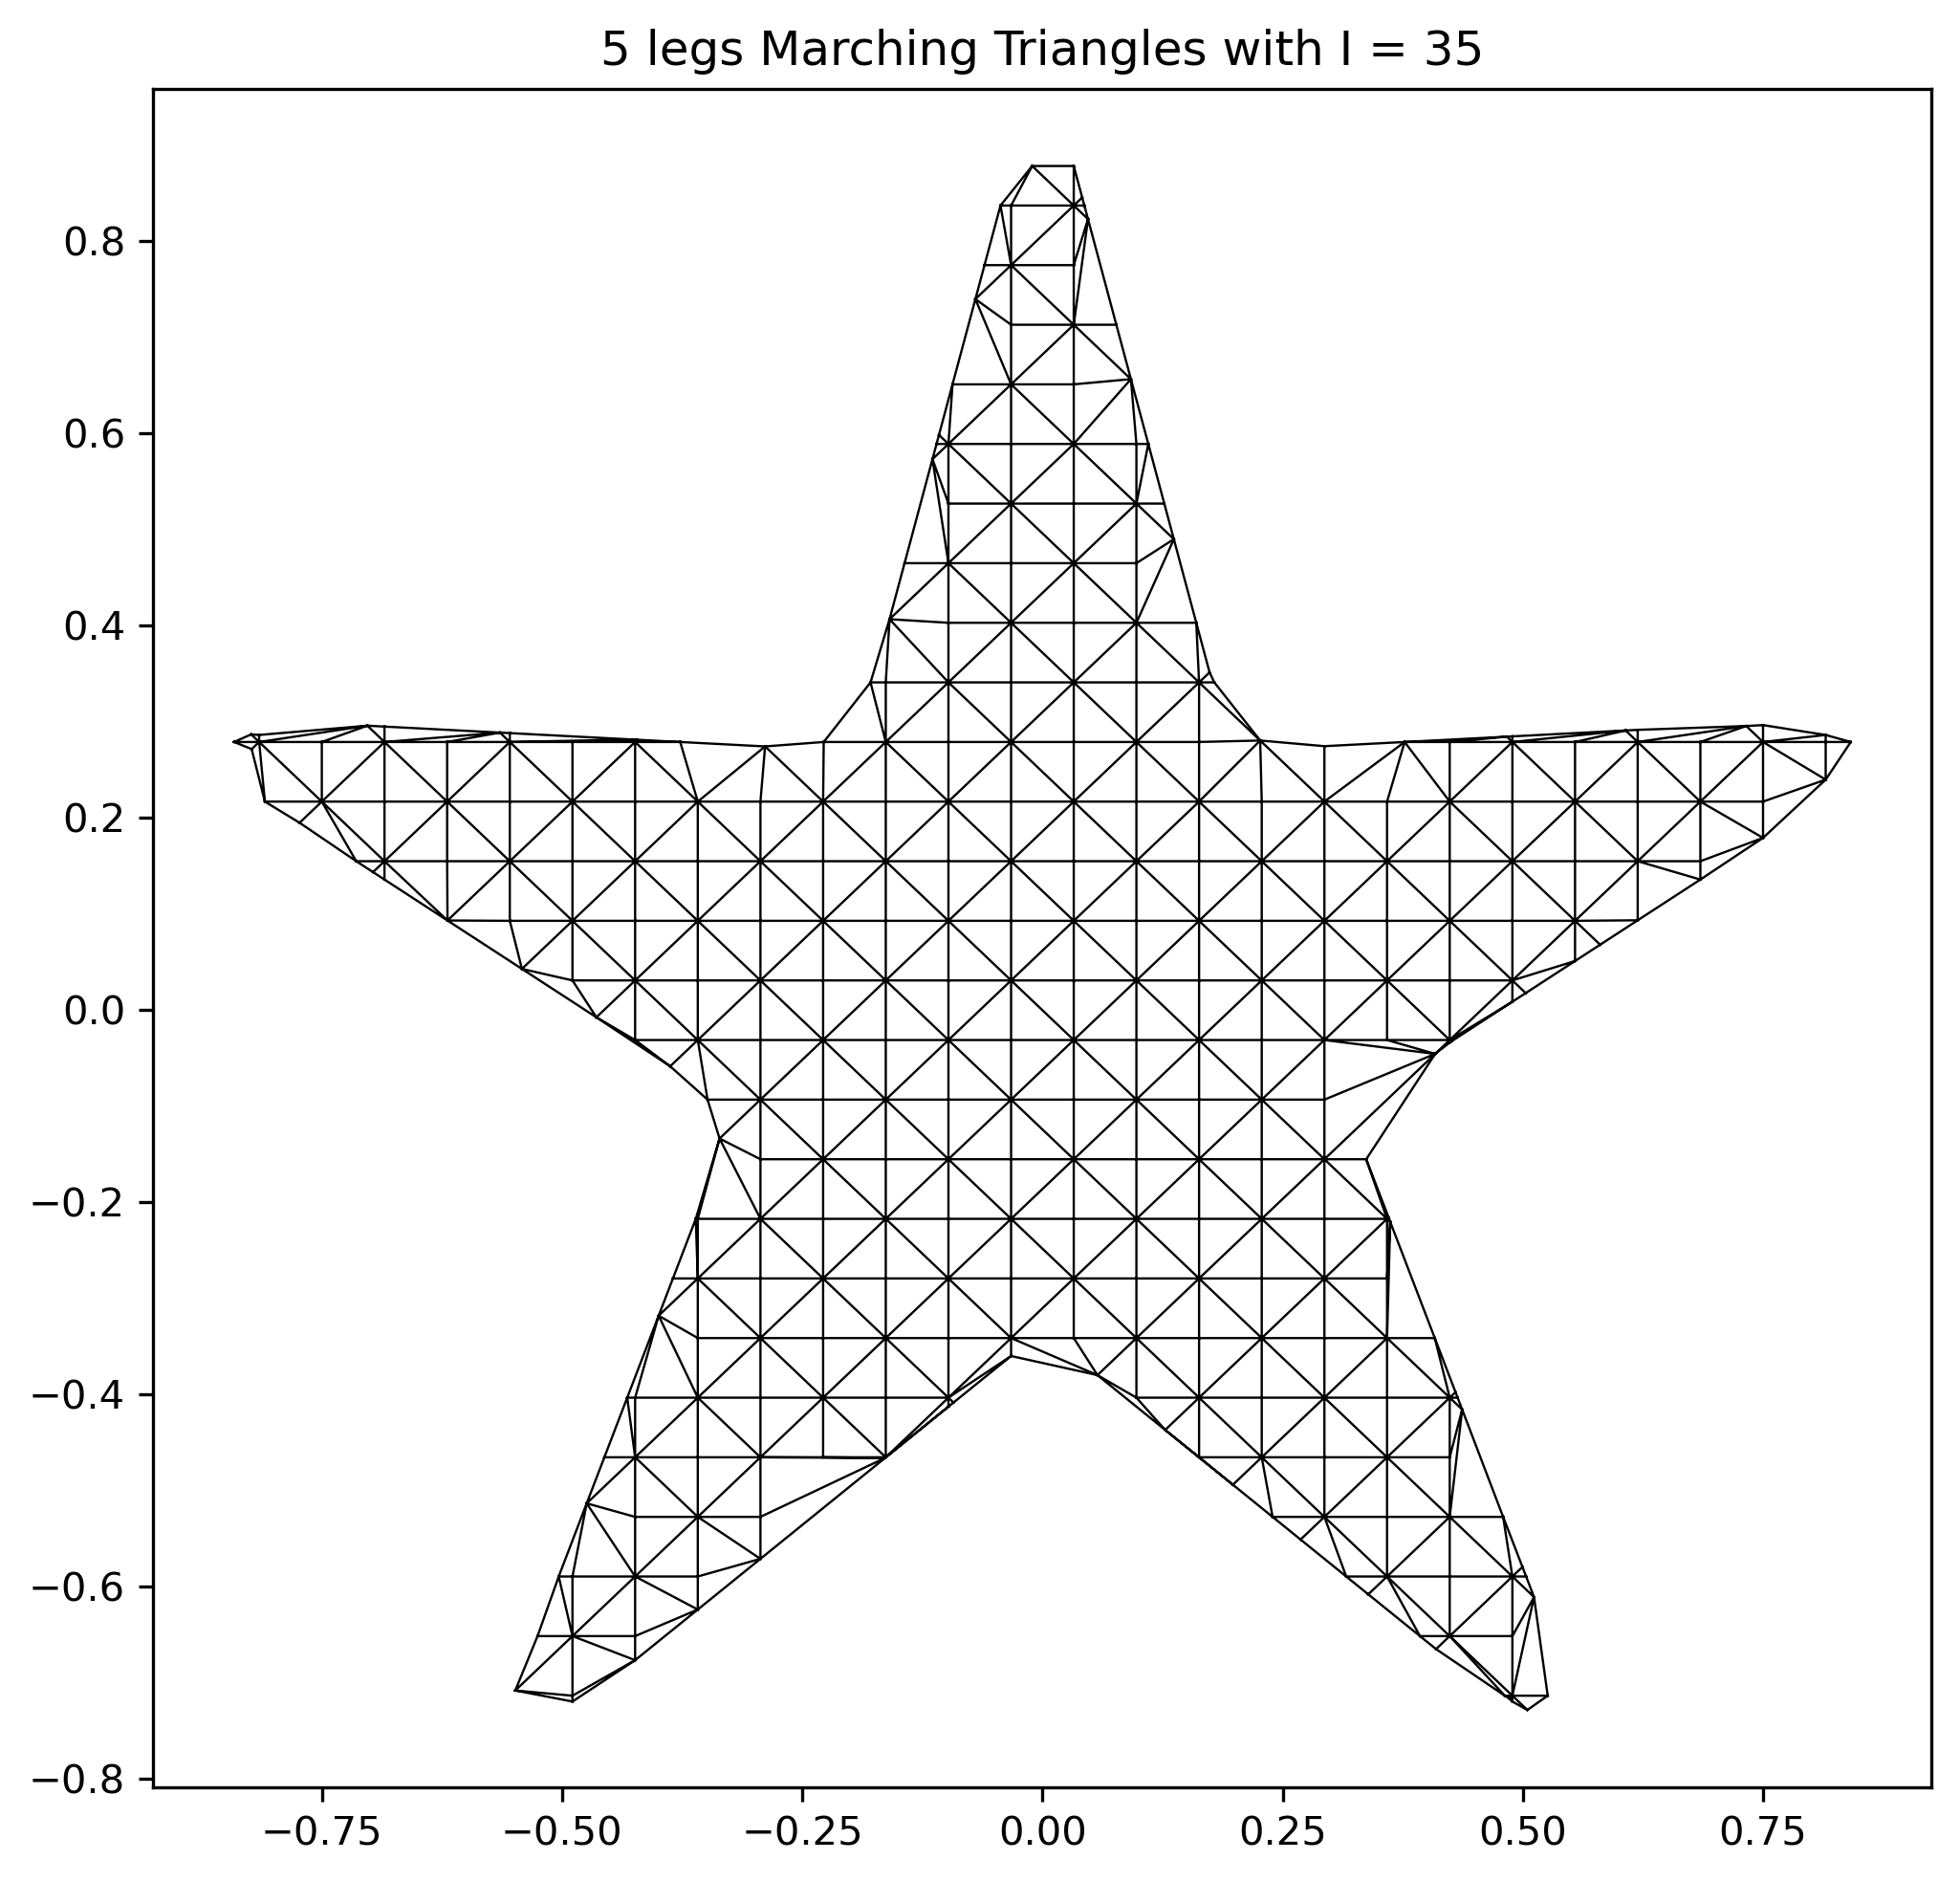
\includegraphics[width=\textwidth]{Images/5 legs Marching Triangles with I = 35.png}
  \end{subfigure}\hfill
  \begin{subfigure}{0.22\textwidth}
    \centering
    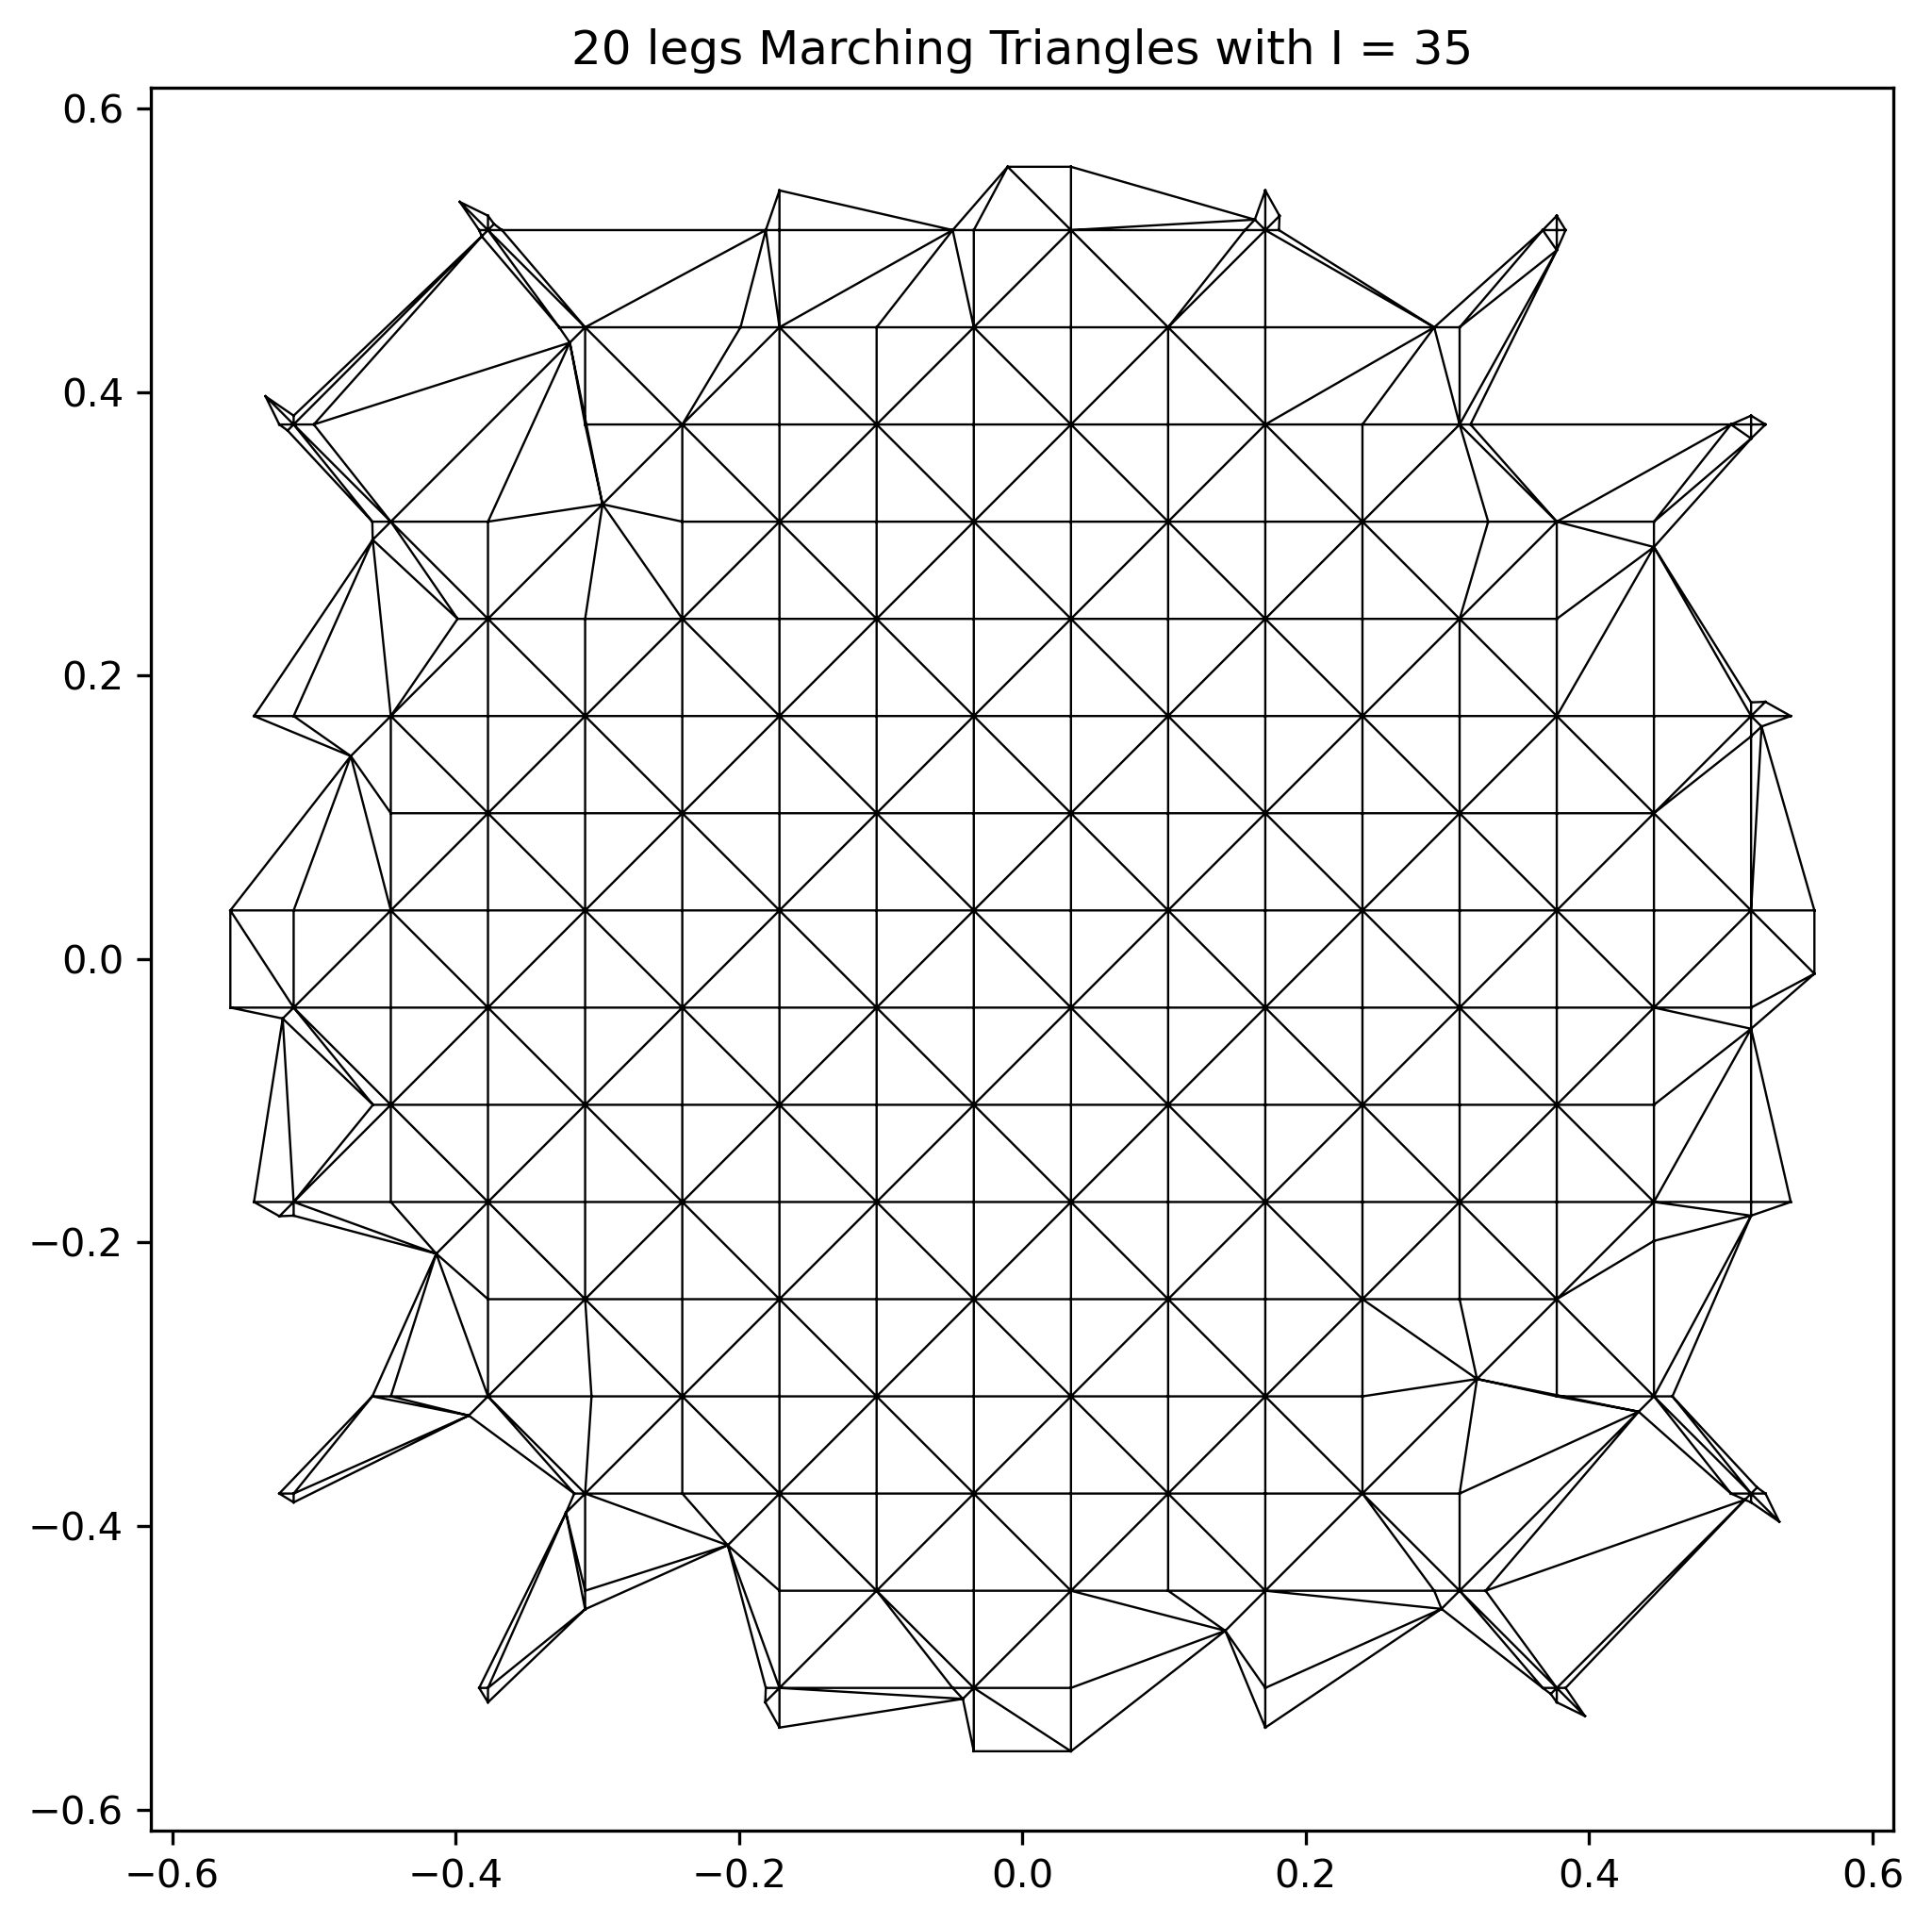
\includegraphics[width=\textwidth]{Images/20 legs Marching Triangles with I = 35.png}
  \end{subfigure}

  \begin{subfigure}{0.22\textwidth}
    \centering
    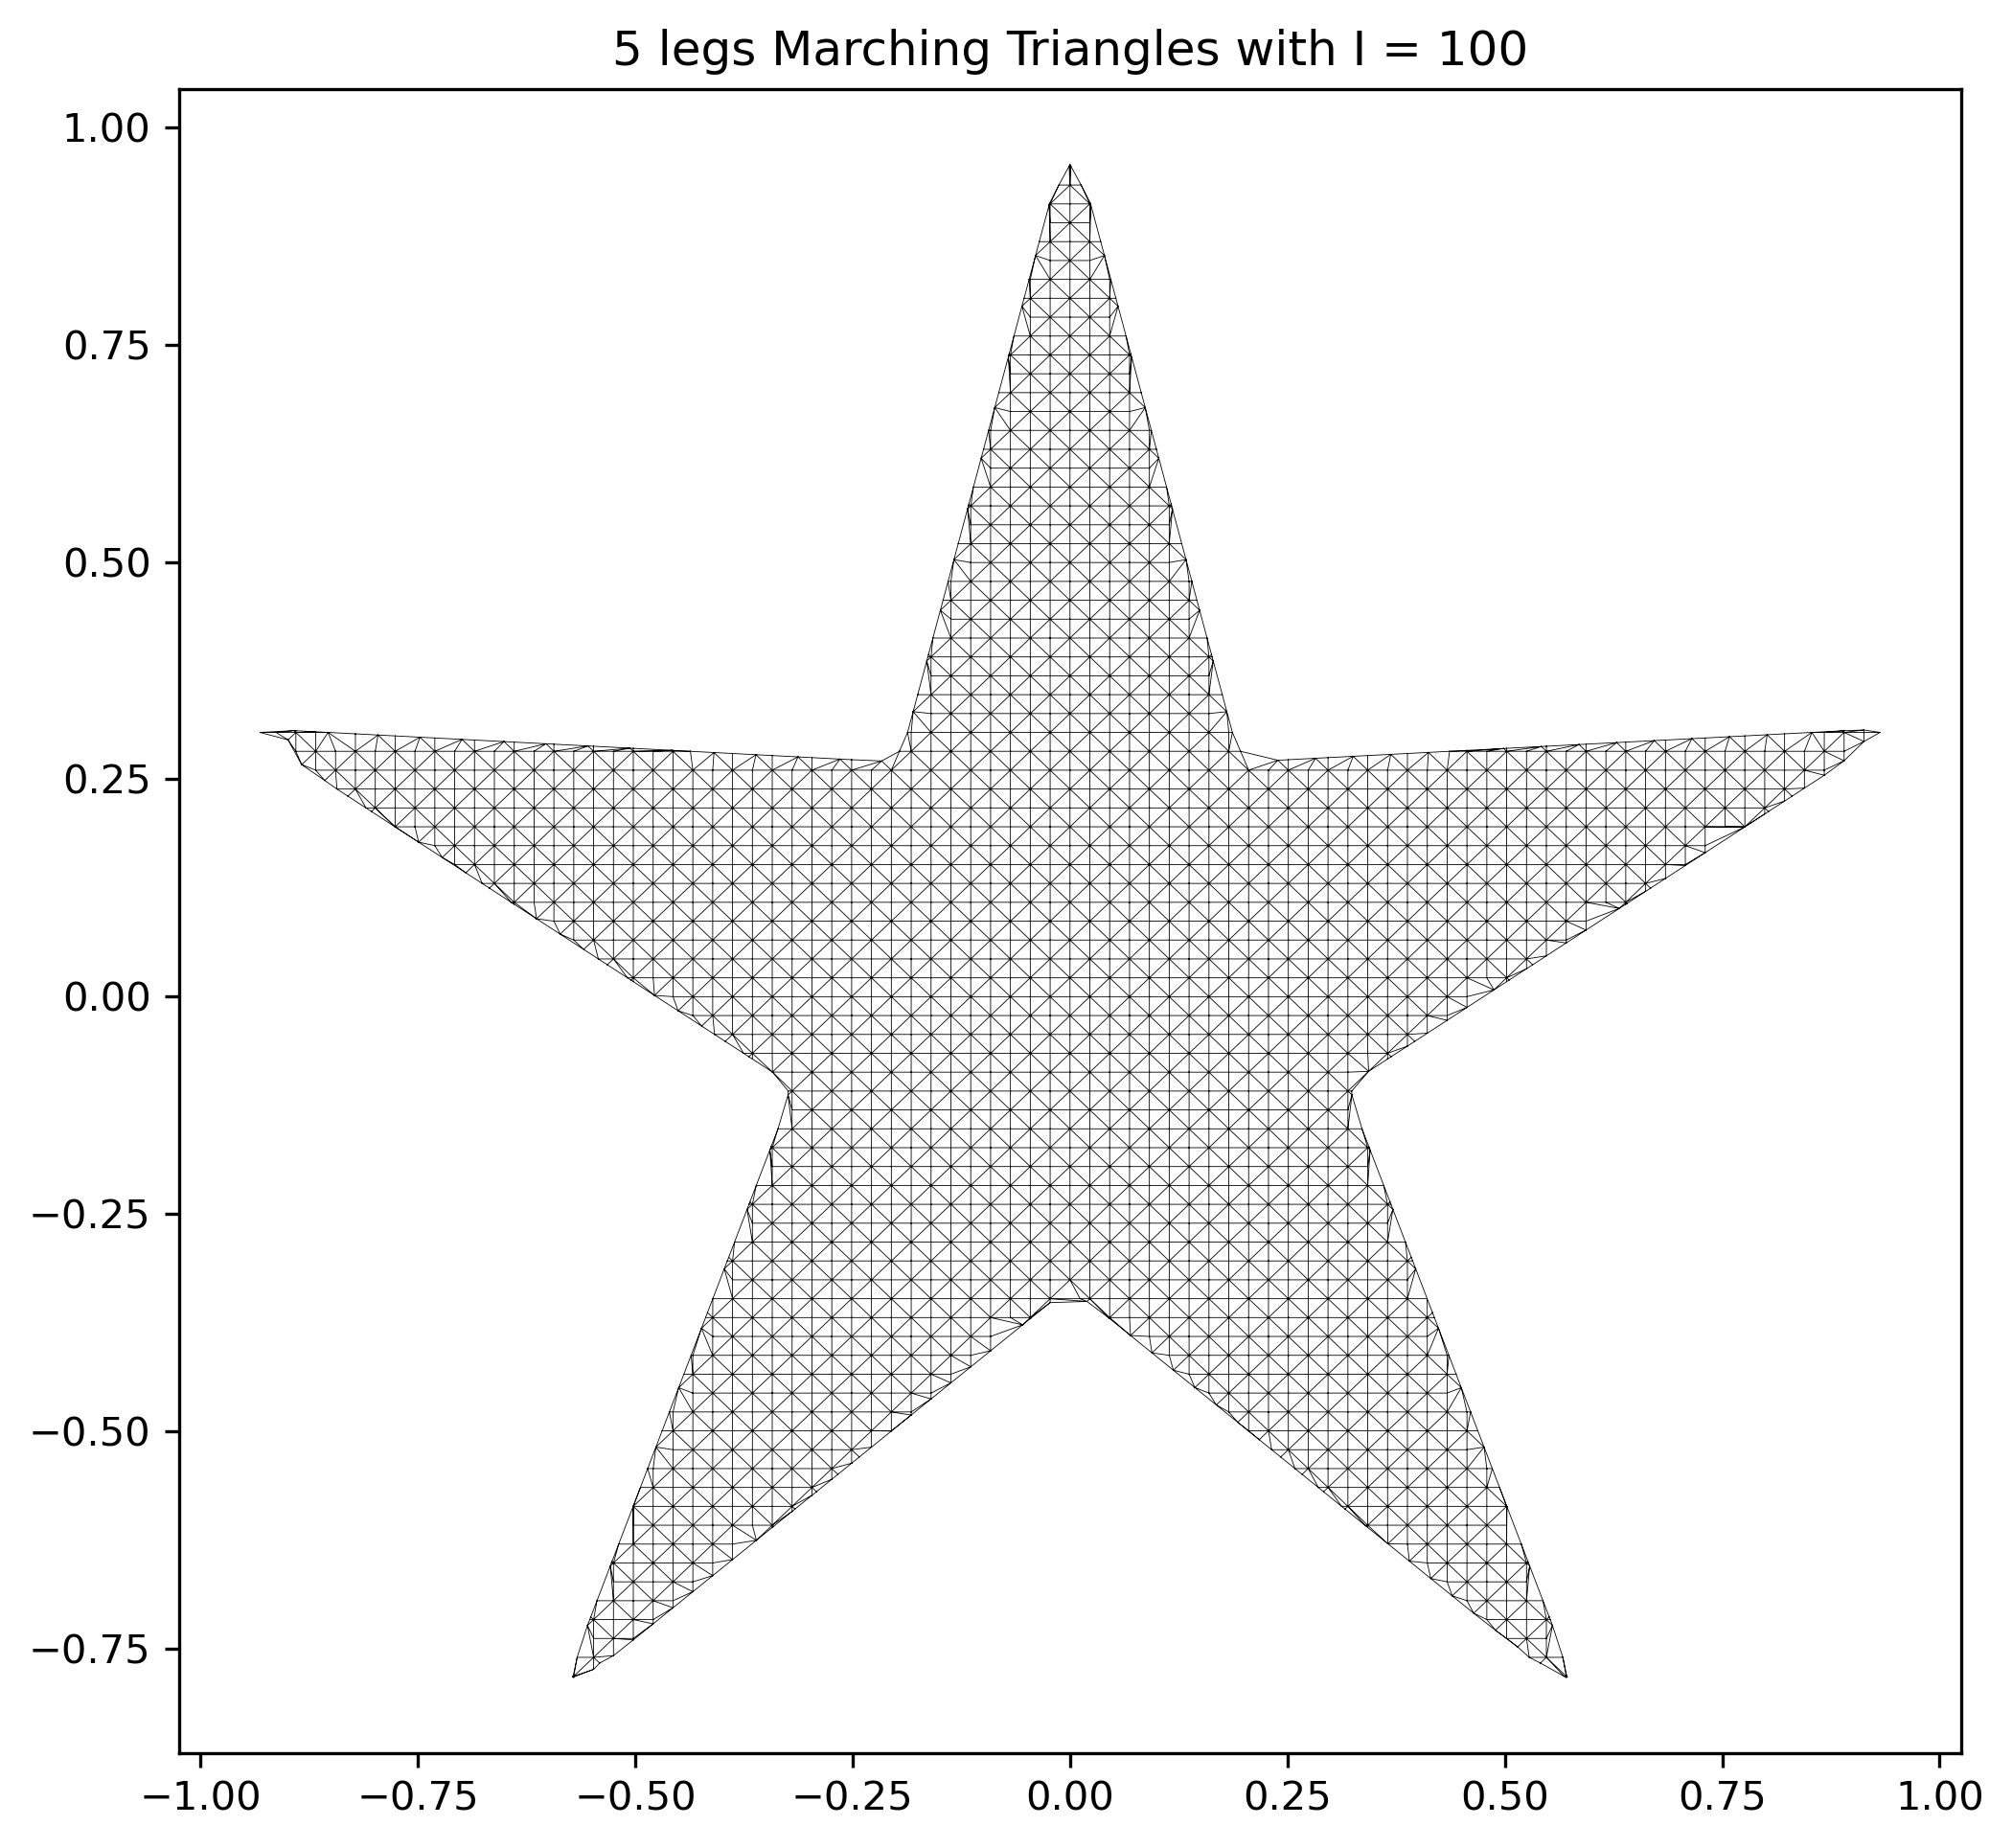
\includegraphics[width=\textwidth]{Images/5 legs Marching Triangles with I = 100.png}
  \end{subfigure}\hfill
  \begin{subfigure}{0.22\textwidth}
    \centering
    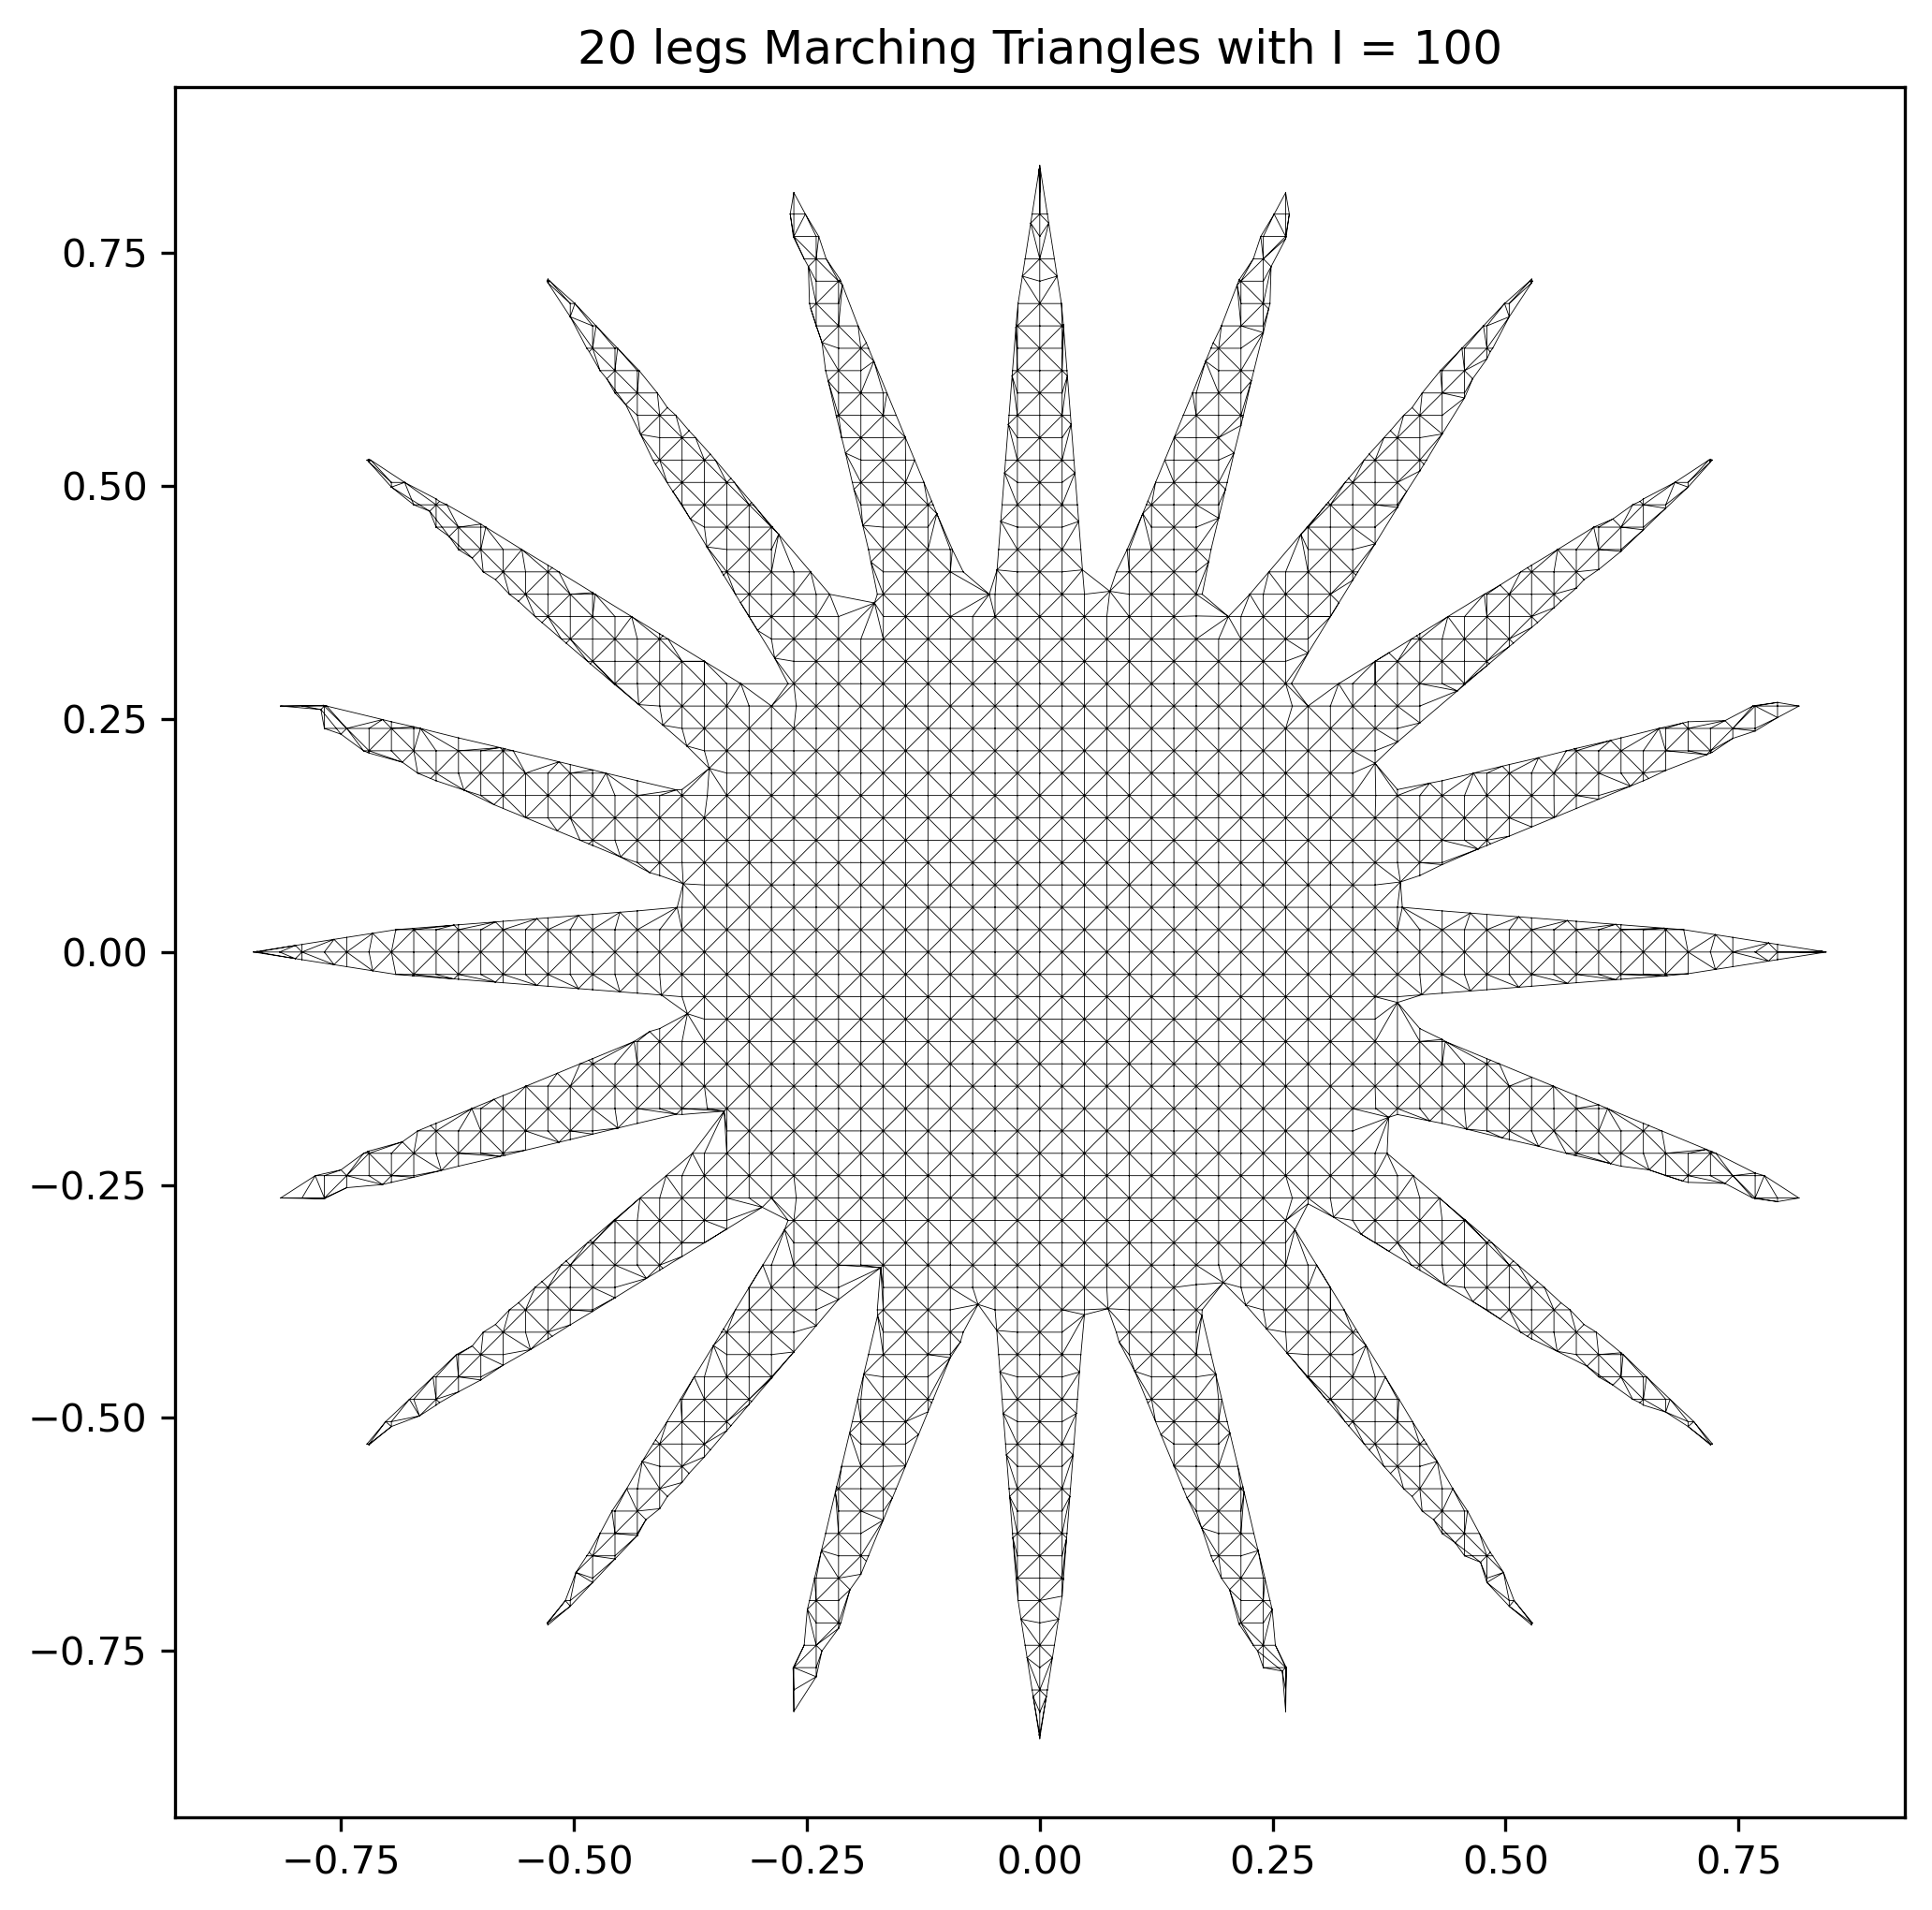
\includegraphics[width=\textwidth]{Images/20 legs Marching Triangles with I = 100.png}
  \end{subfigure}
  \caption{Result of our marching triangles alogrithm for the 5- and 20-legged star shapes, both done for grid sizes $I = 100$ and $I = 35$. Wee see that, for low grid sizes, our algorithm has a very hard time with fine edges, and the 20-legged star shape is basically unrecognizable. This happens in part due to the way we project the triangle vertices, and the fact that the vertices of any one triangle on our intial mesh might be in two completely different parts of the shape due to the grid size being way larger than the thickness of the arms of the star in this case. When we project the triangle vertices onto the 0 contour of the SDF, we assume that the directional gradient of the SDF is constant along the line on which we project the points, which is generally not true, and depends on the shape of the polygon. This causes inaccuracies, and in the worst cases, if the grid is not very fine, complete failure to capture the relevant geometry.}
\end{figure}

\begin{figure}[H]
  \centering
  \begin{subfigure}{0.22\textwidth}
    \centering
    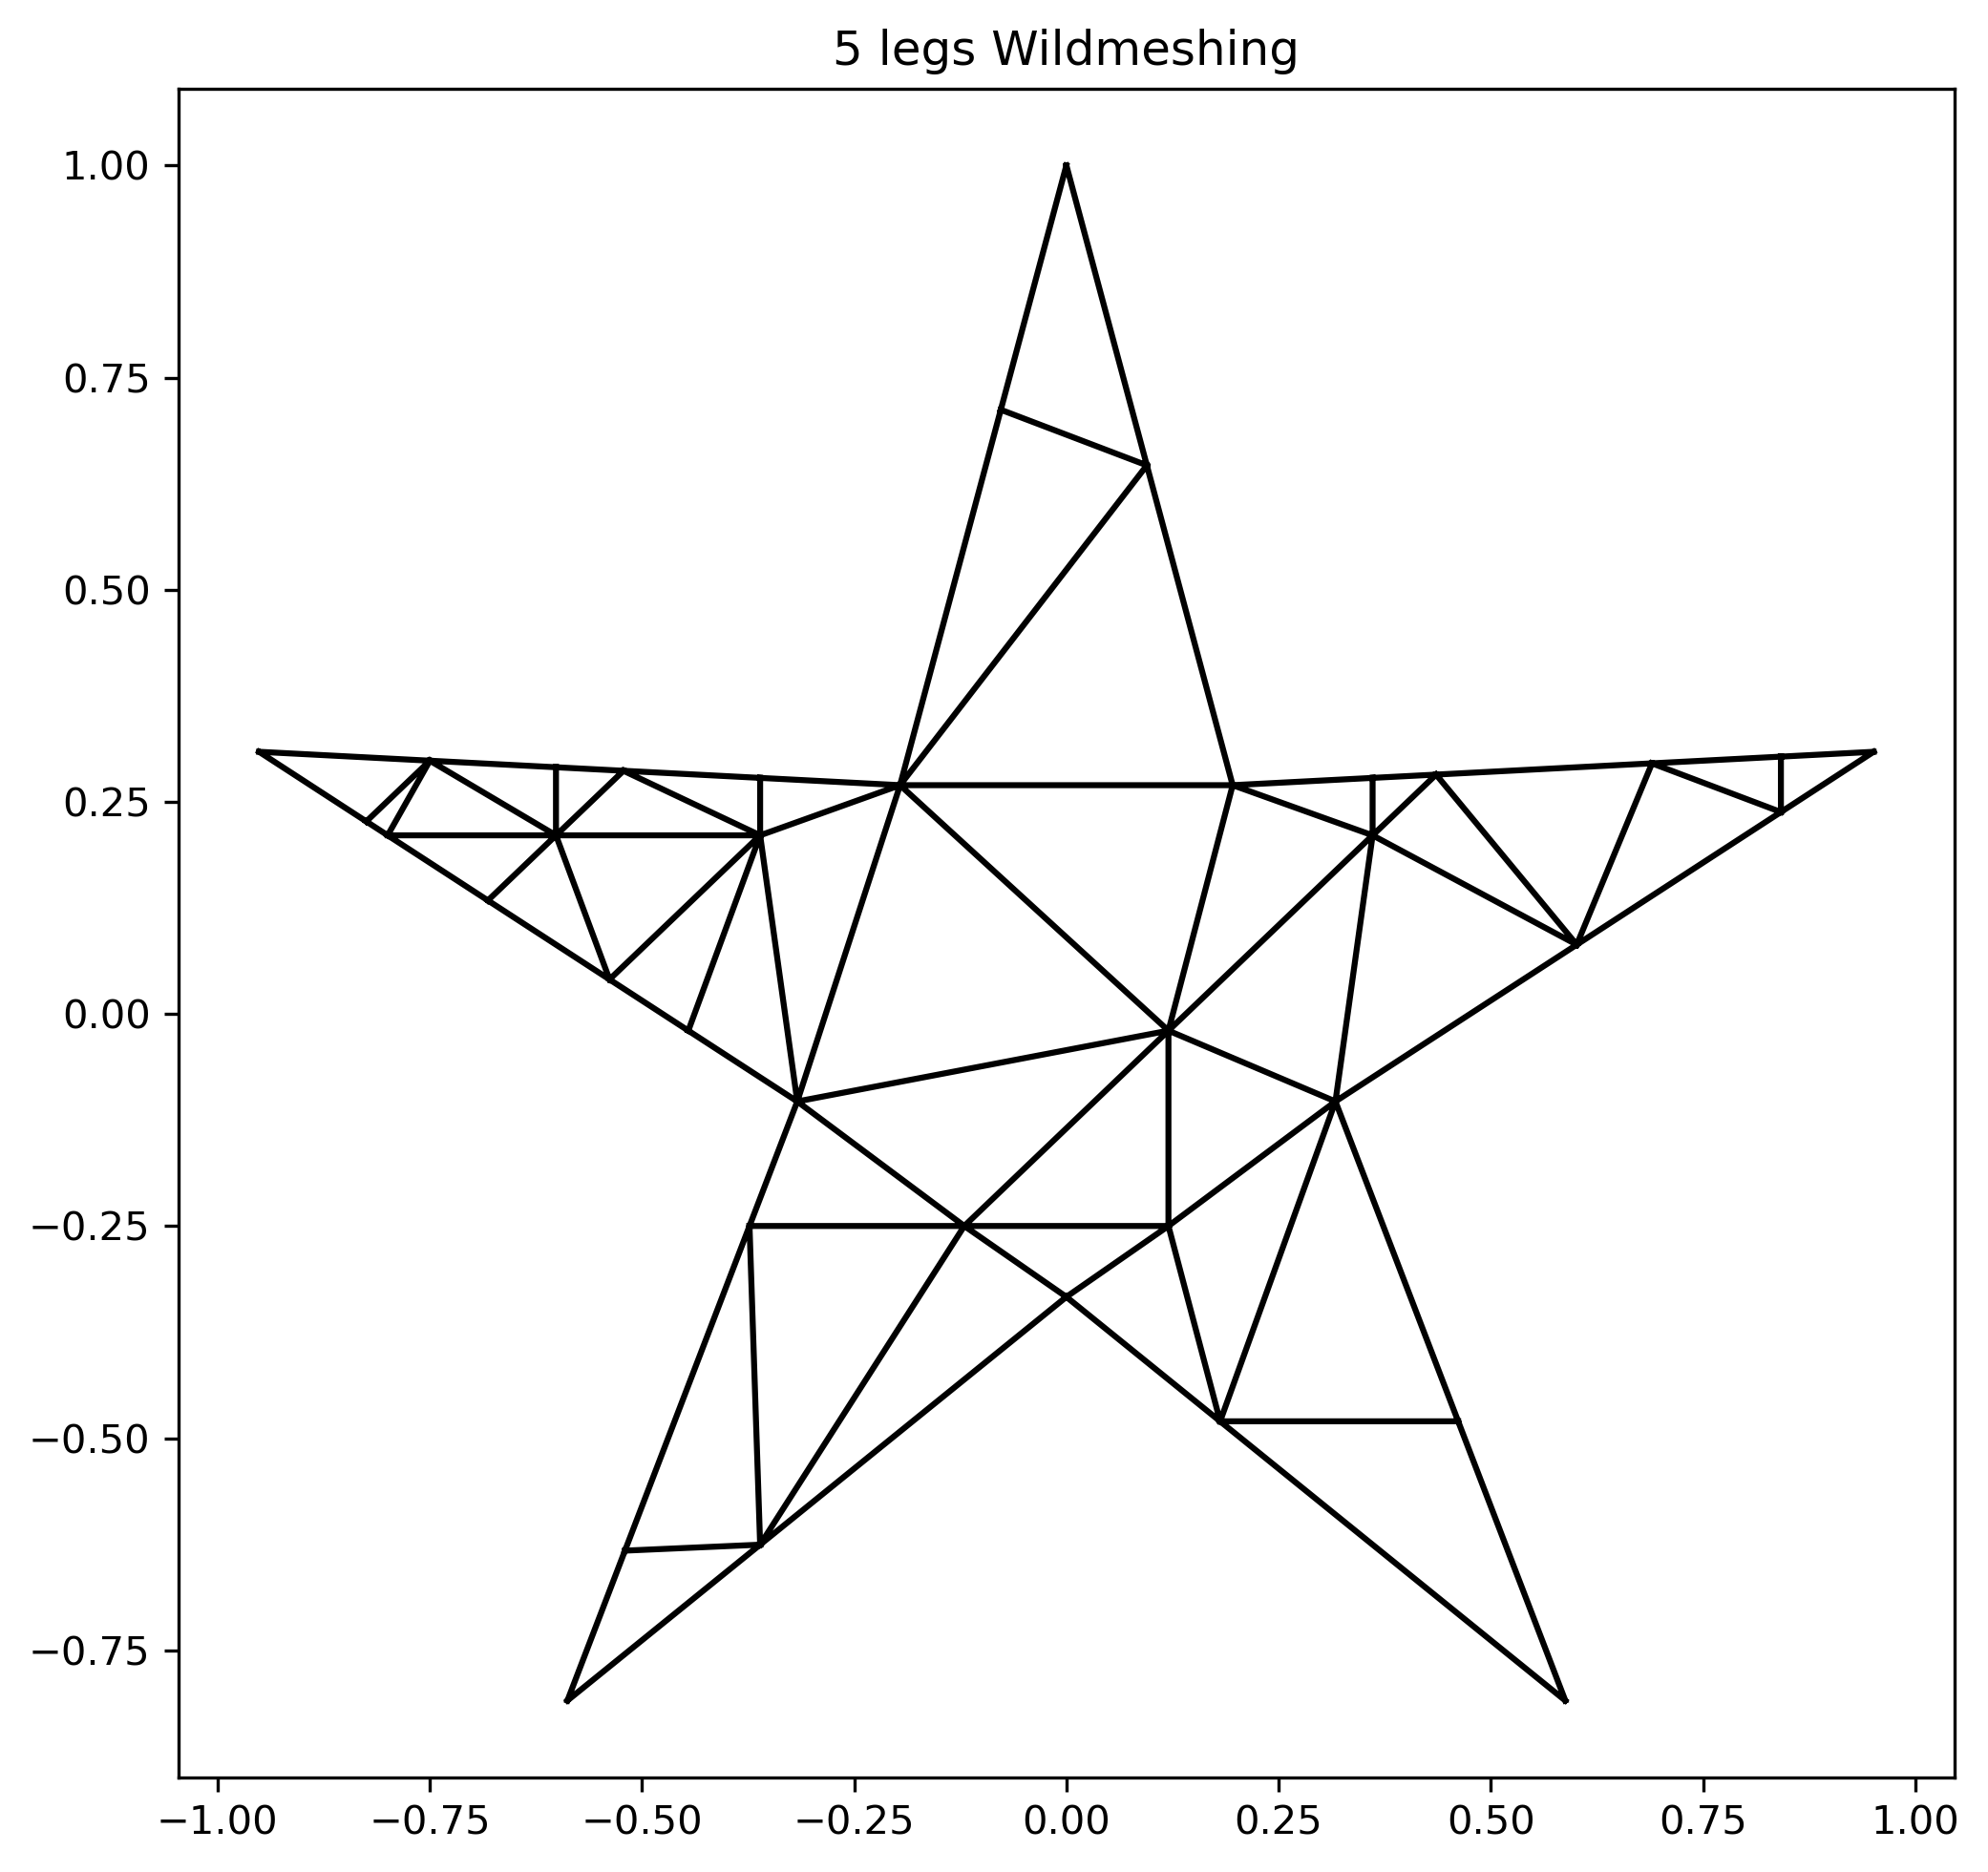
\includegraphics[width=\textwidth]{Images/5 legs Wildmeshing.png}
  \end{subfigure}
  \begin{subfigure}{0.22\textwidth}
    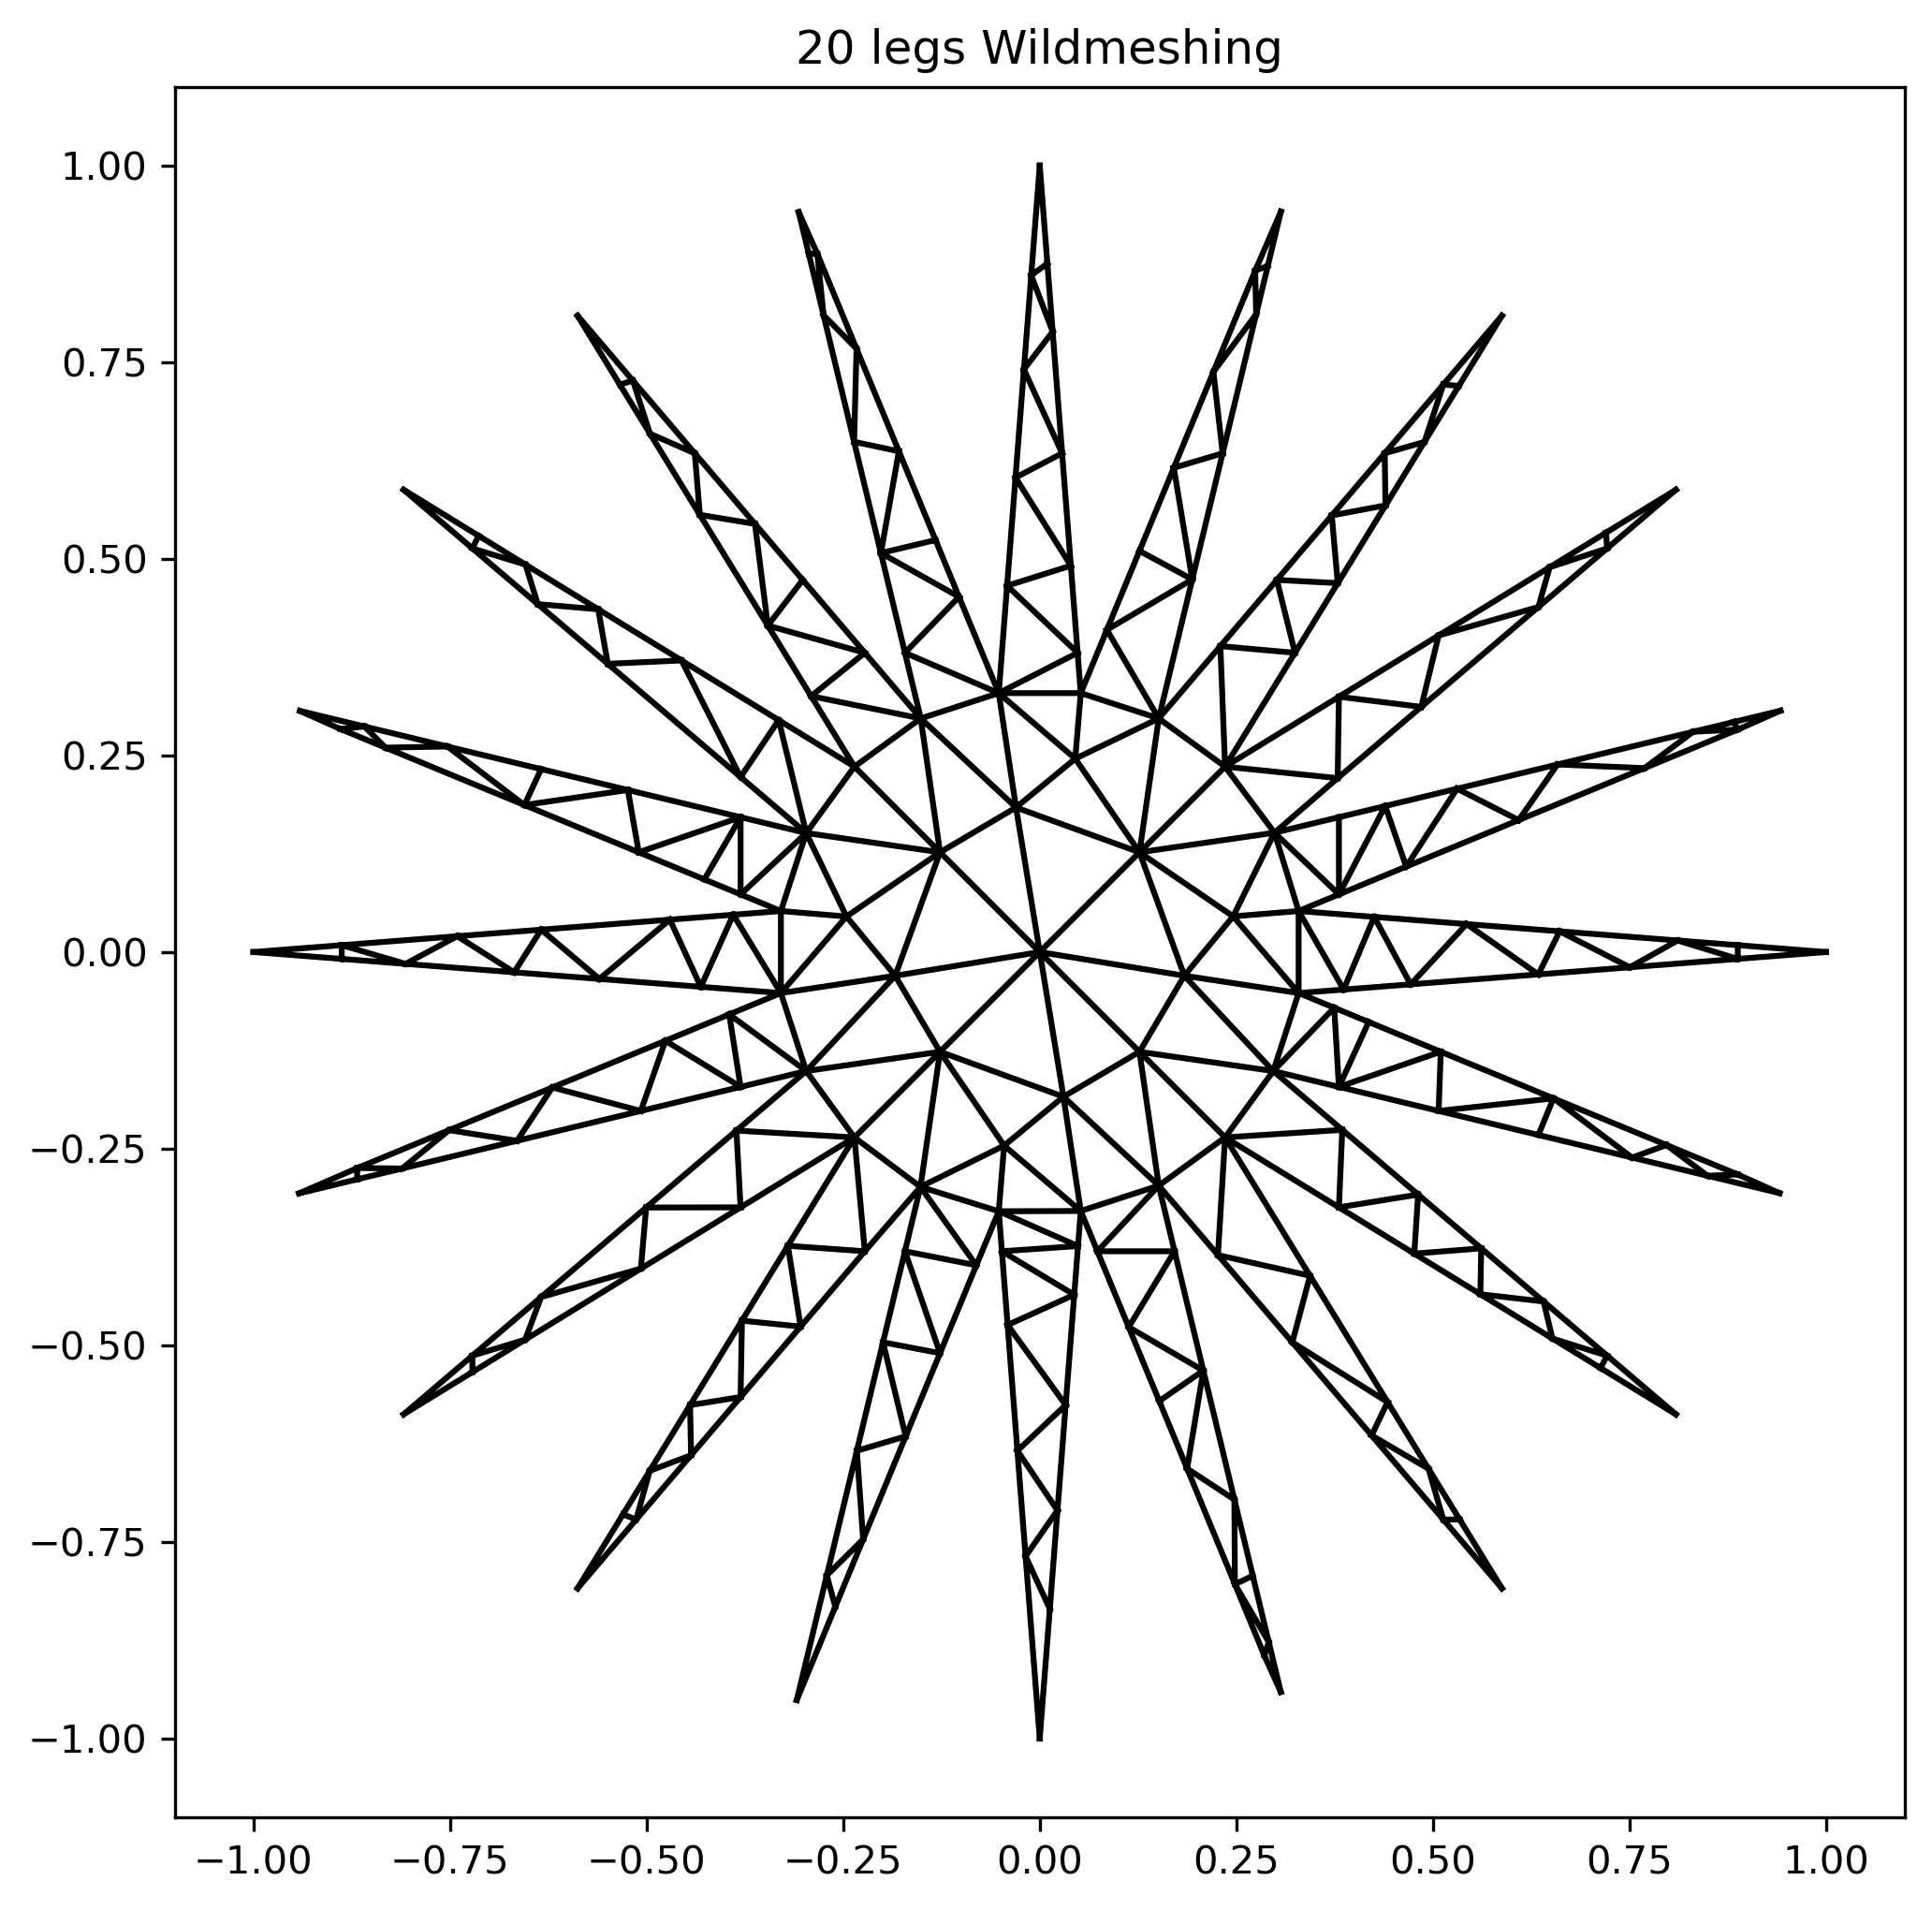
\includegraphics[width=\textwidth]{Images/20 legs Wildmeshing.png}
    \centering
  \end{subfigure}\hfill
  \caption{Result of the Wildmeshing algorithm on the 5-legged and 20-legged stars. We see that the number of triangles needed to acurately conform to the shape of the polygon is actually much less than in our marching triangles algorithm, hinting at some much needed optimization in our algorithm.}
\end{figure}

\newpage
\section{Mesh quality comparison}
In this section we'll compare the quality of the meshes generated by the
different algorithms using the quality measures we looked at in the beginning
of the report. We'll plot histograms of the radius and area ratios for the
different meshes.
\begin{figure}[H]
  \centering
  \begin{subfigure}{0.22\textwidth}
    \centering
    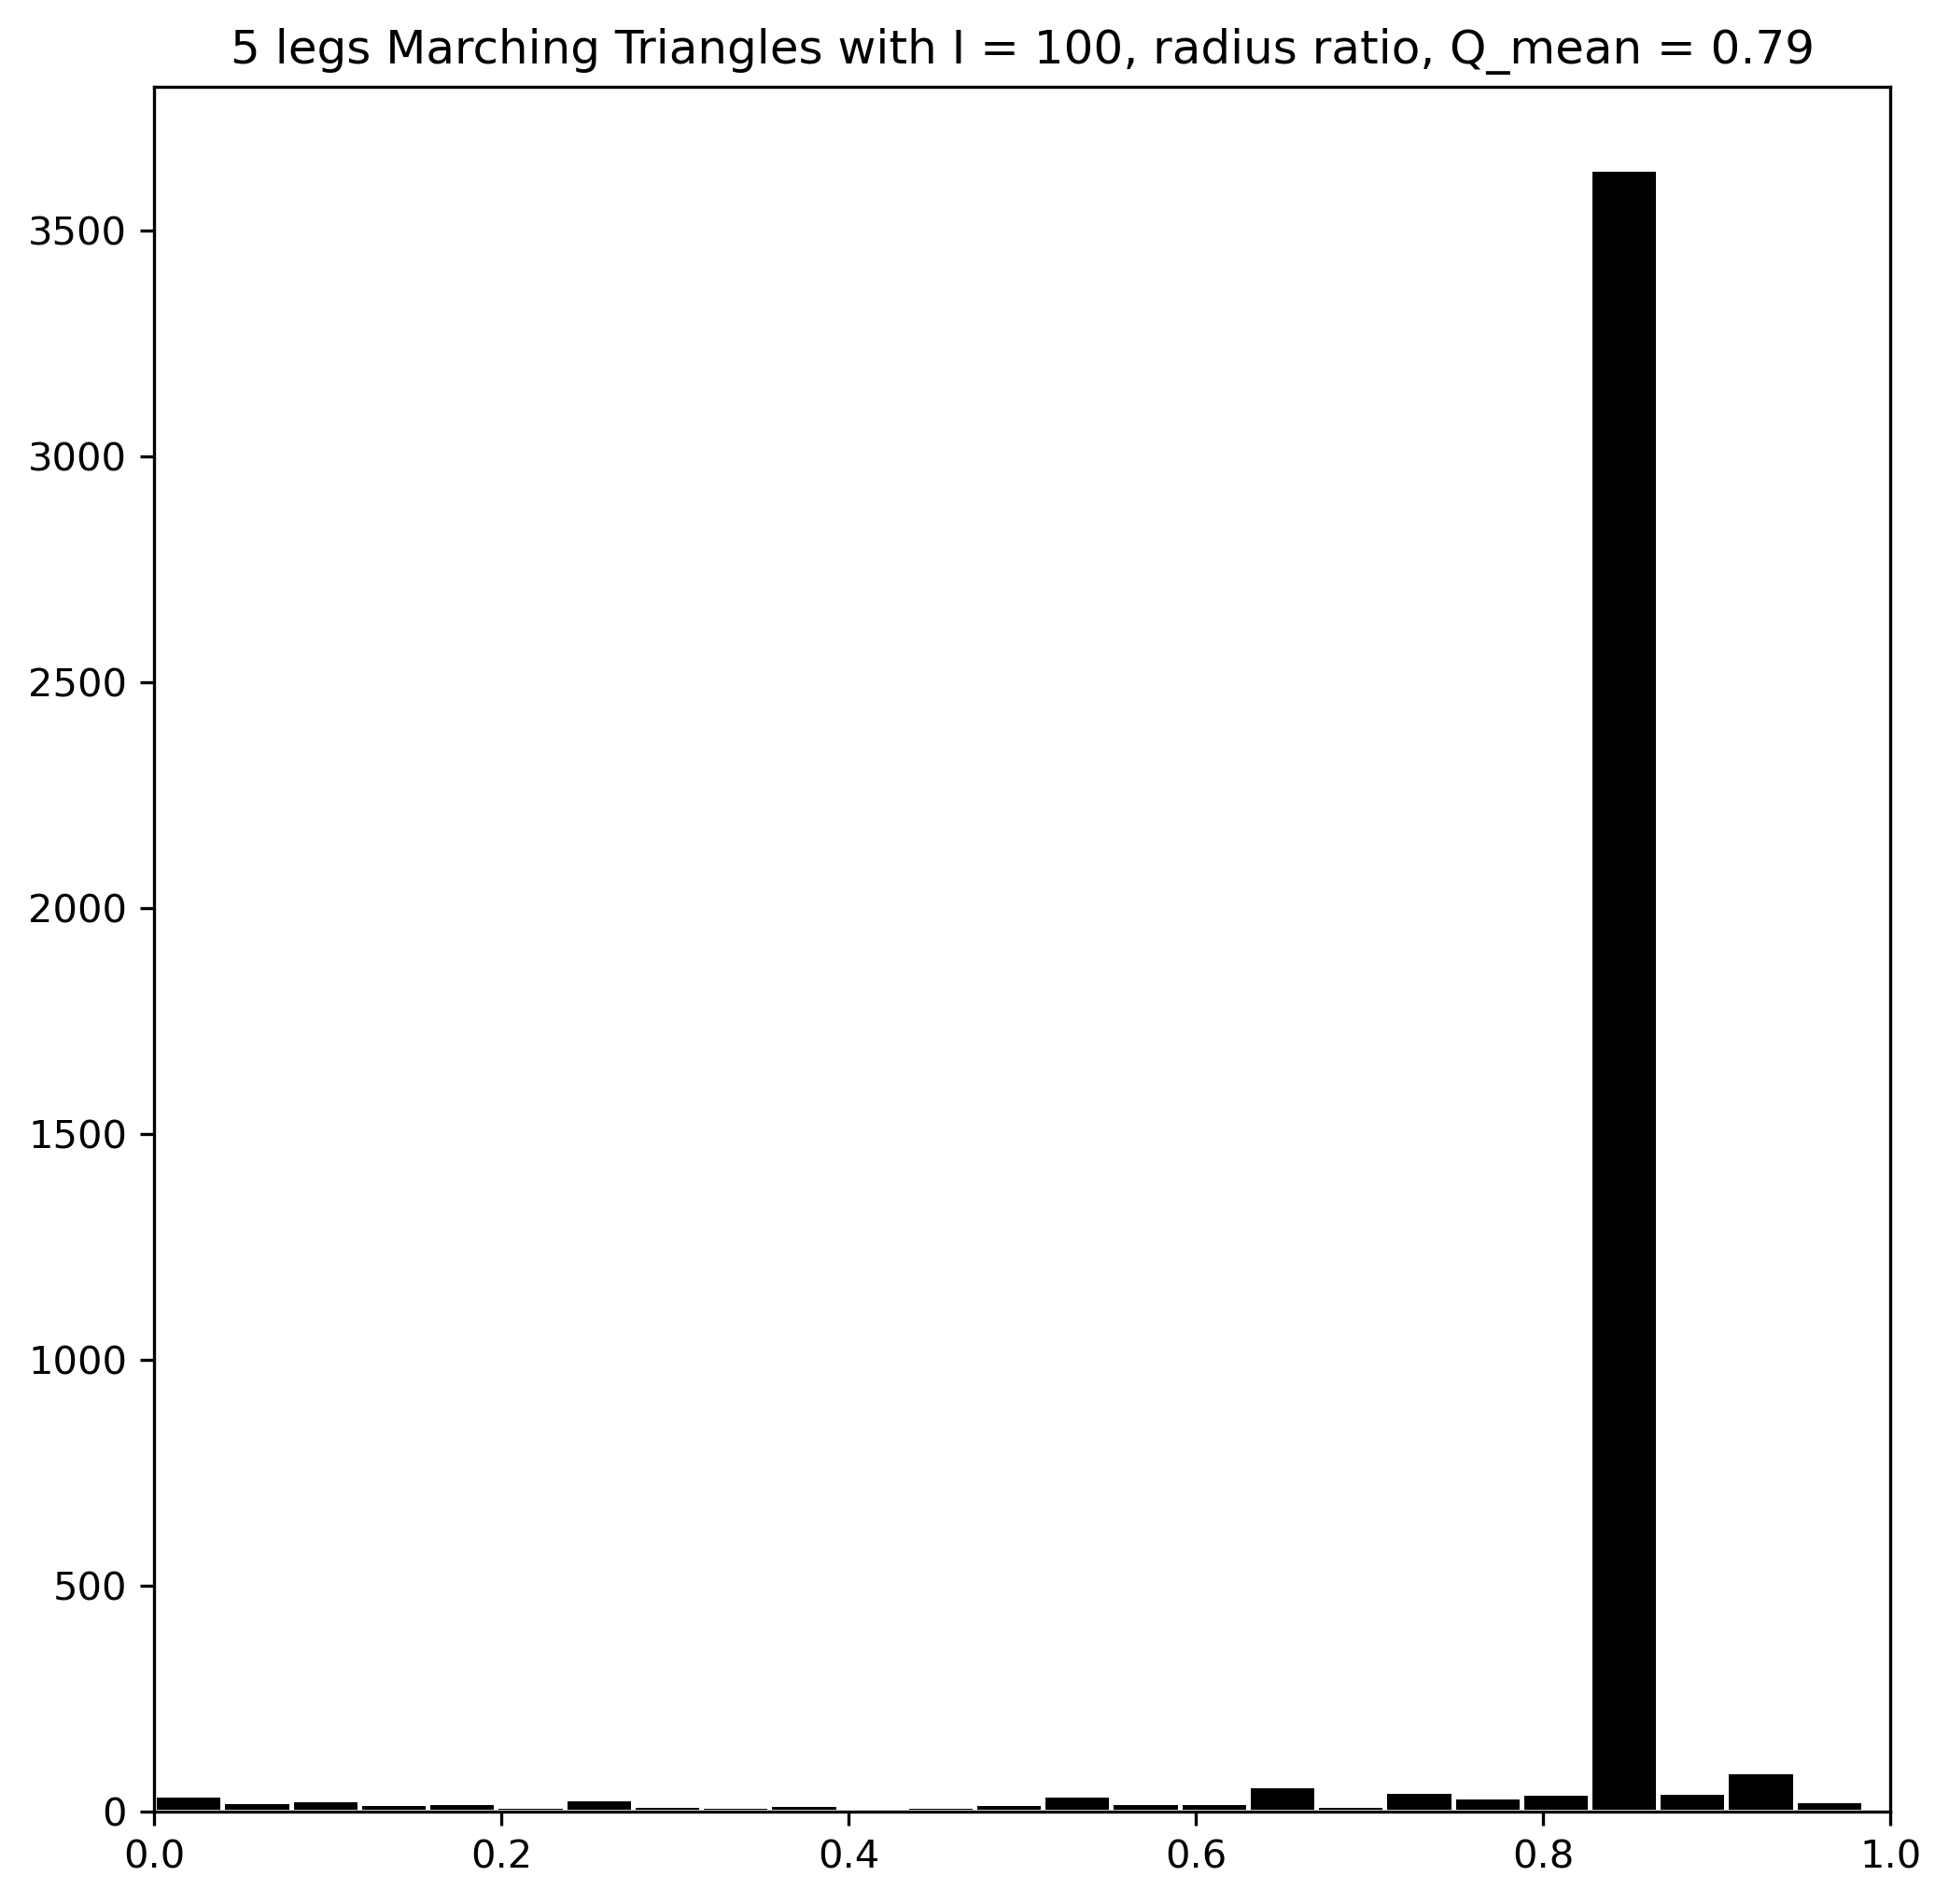
\includegraphics[width=\textwidth]{Images/histograms/5 legs Marching Triangles with I = 100, radius ratio.png}
  \end{subfigure}\hfill
  \begin{subfigure}{0.22\textwidth}
    \centering
    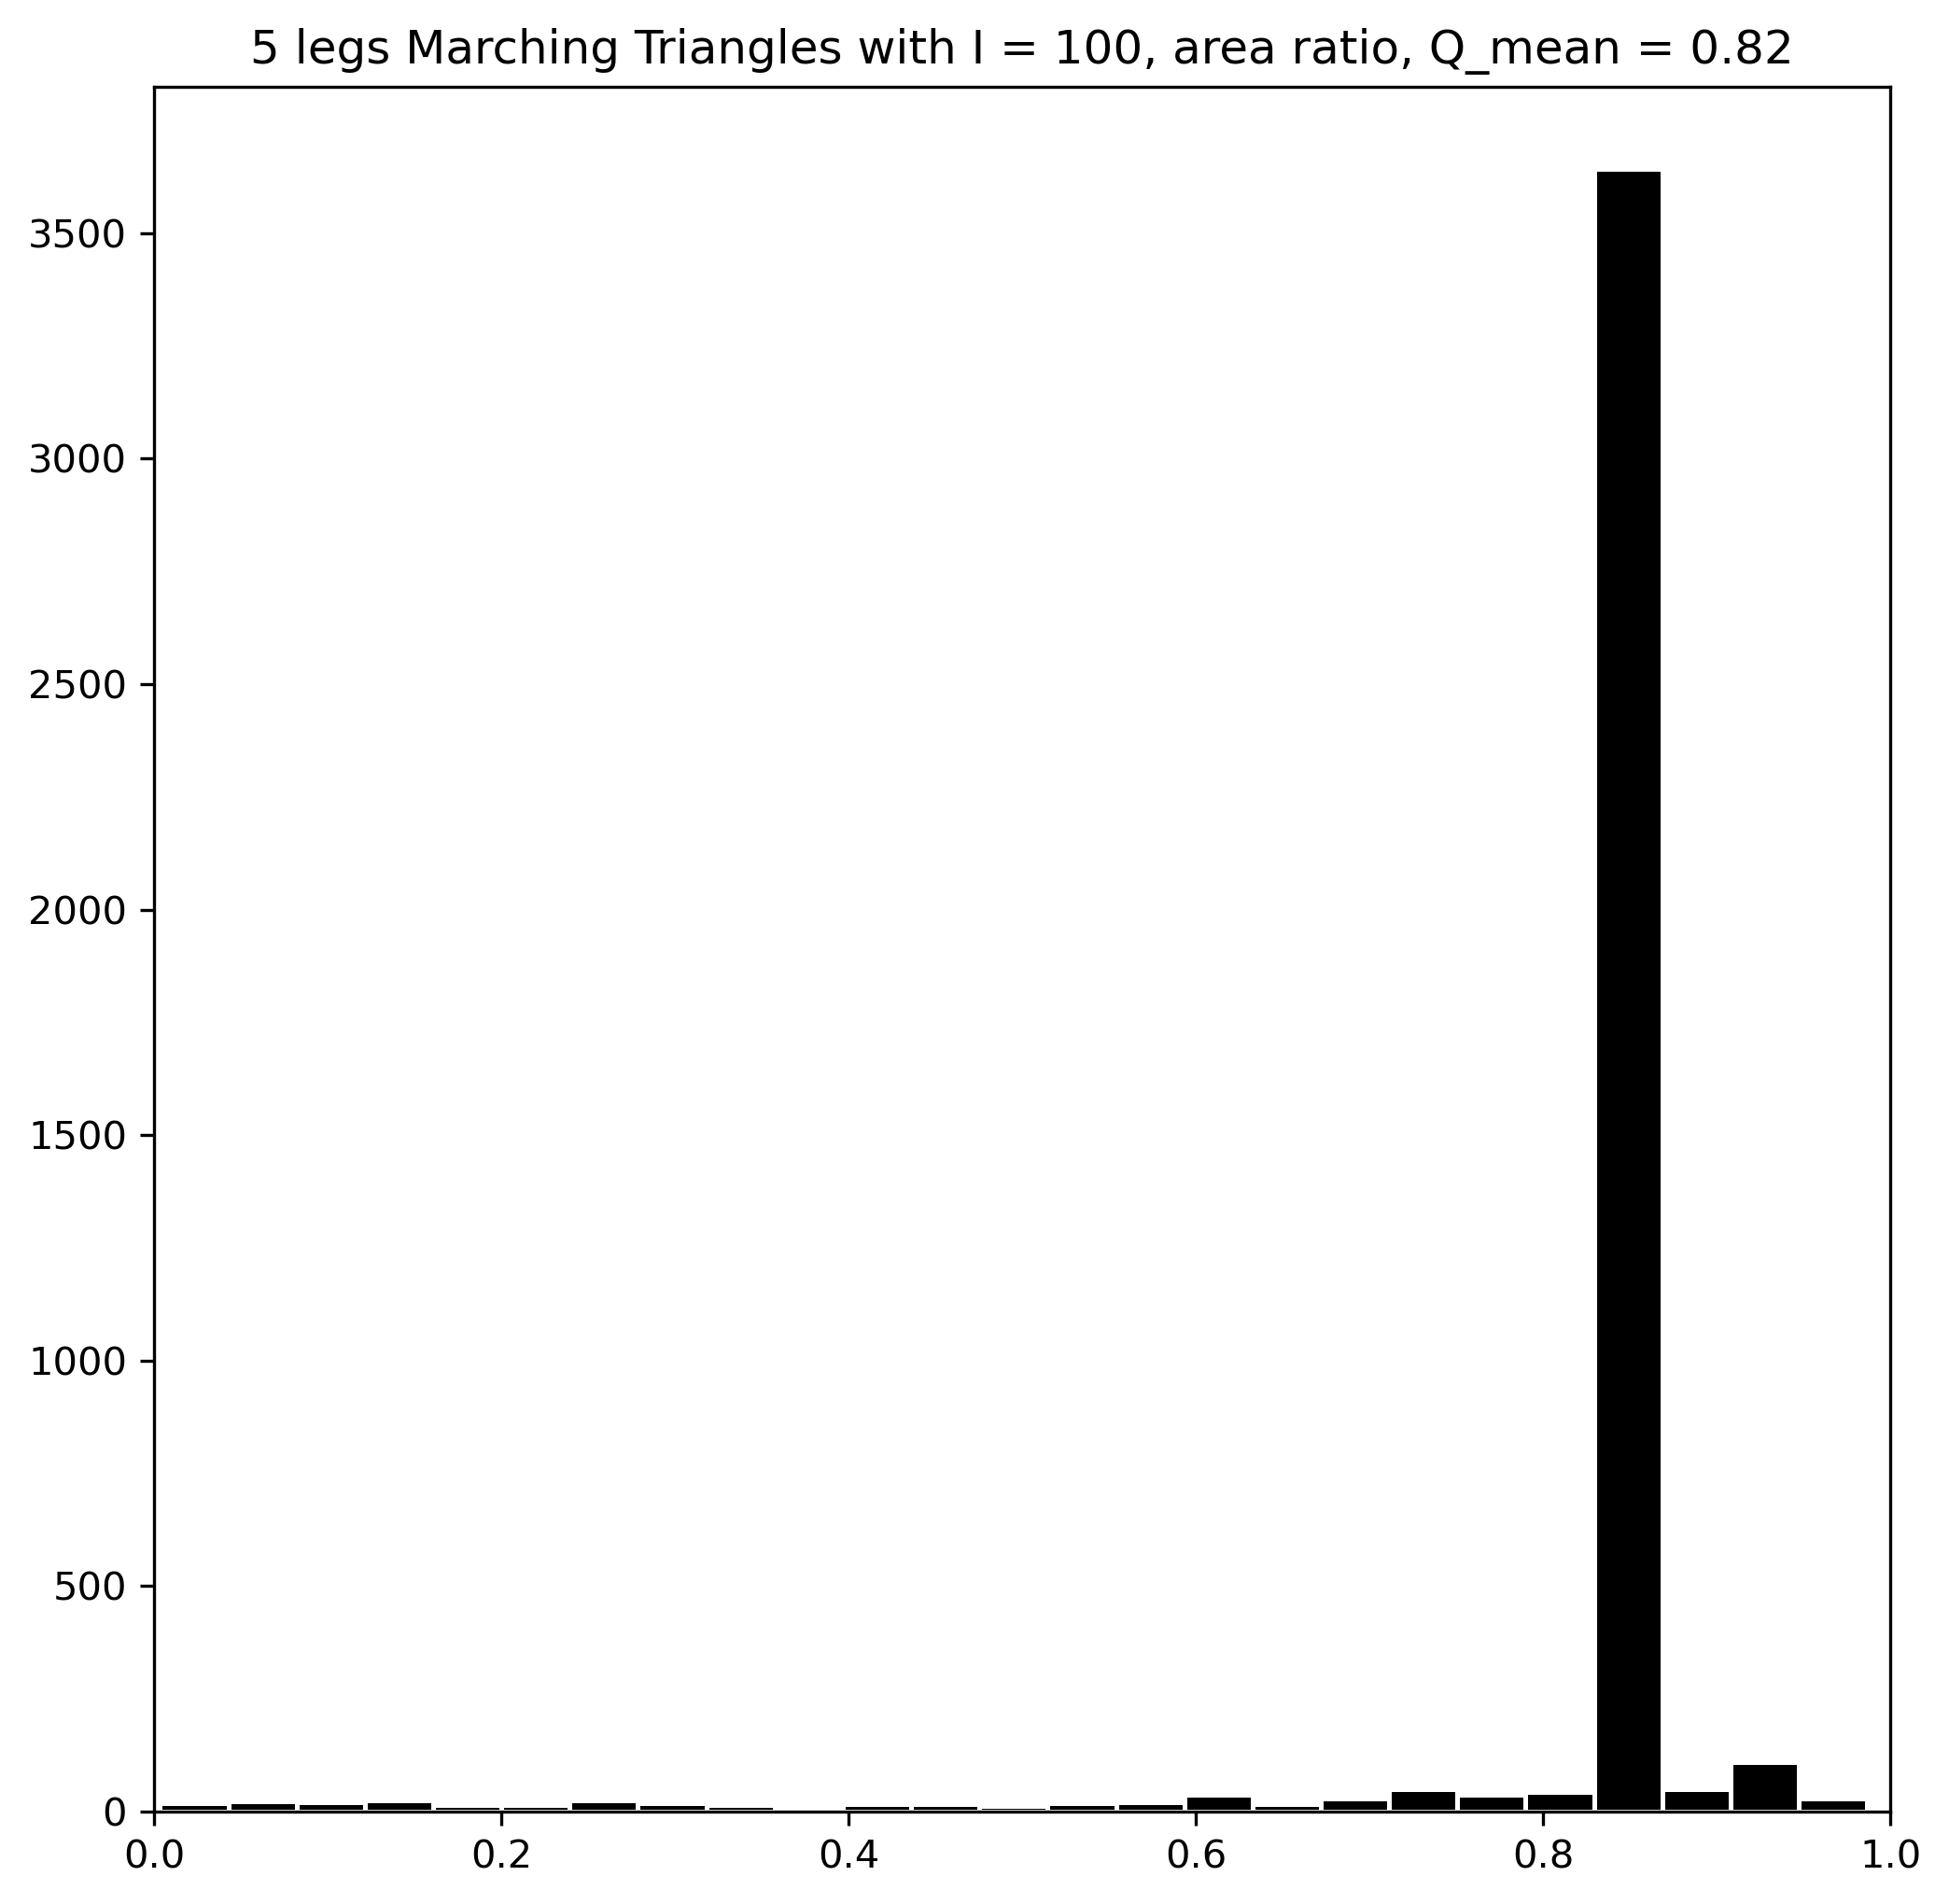
\includegraphics[width=\textwidth]{Images/histograms/5 legs Marching Triangles with I = 100, area ratio.png}
  \end{subfigure}
  \begin{subfigure}{0.22\textwidth}
    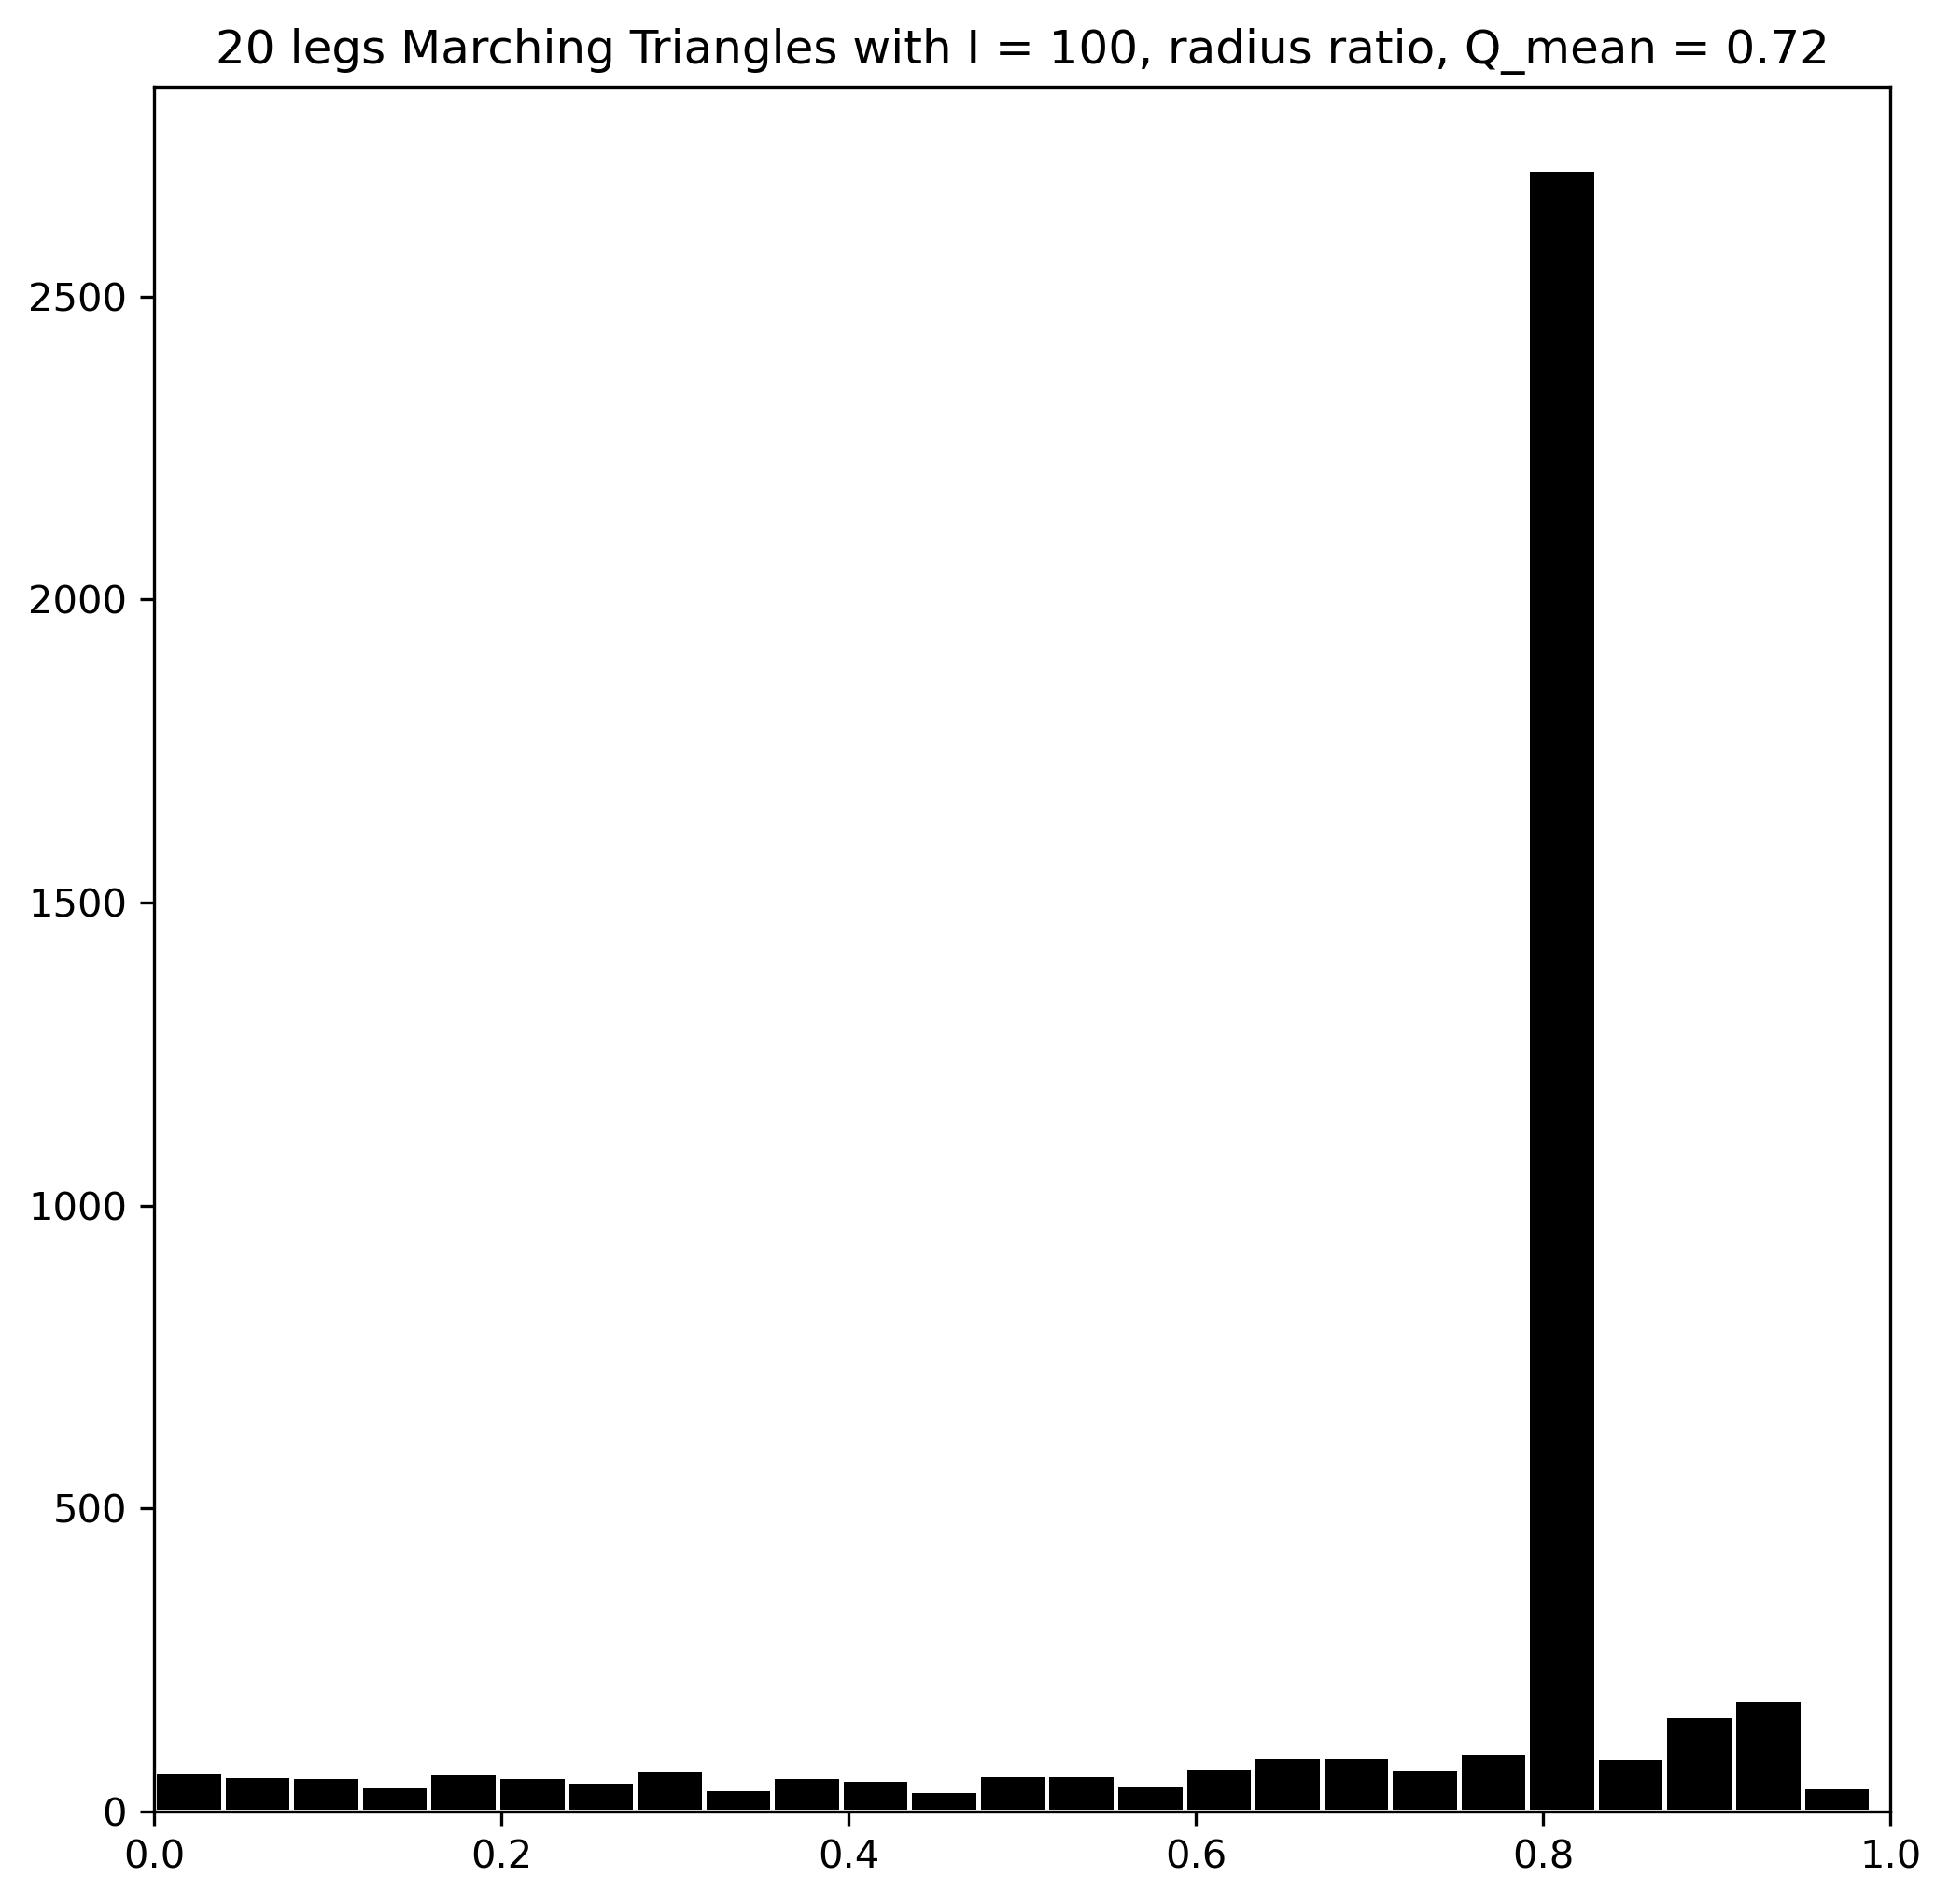
\includegraphics[width=\textwidth]{Images/histograms/20 legs Marching Triangles with I = 100, radius ratio.png}
    \centering
  \end{subfigure}\hfill
  \begin{subfigure}{0.22\textwidth}
    \centering
    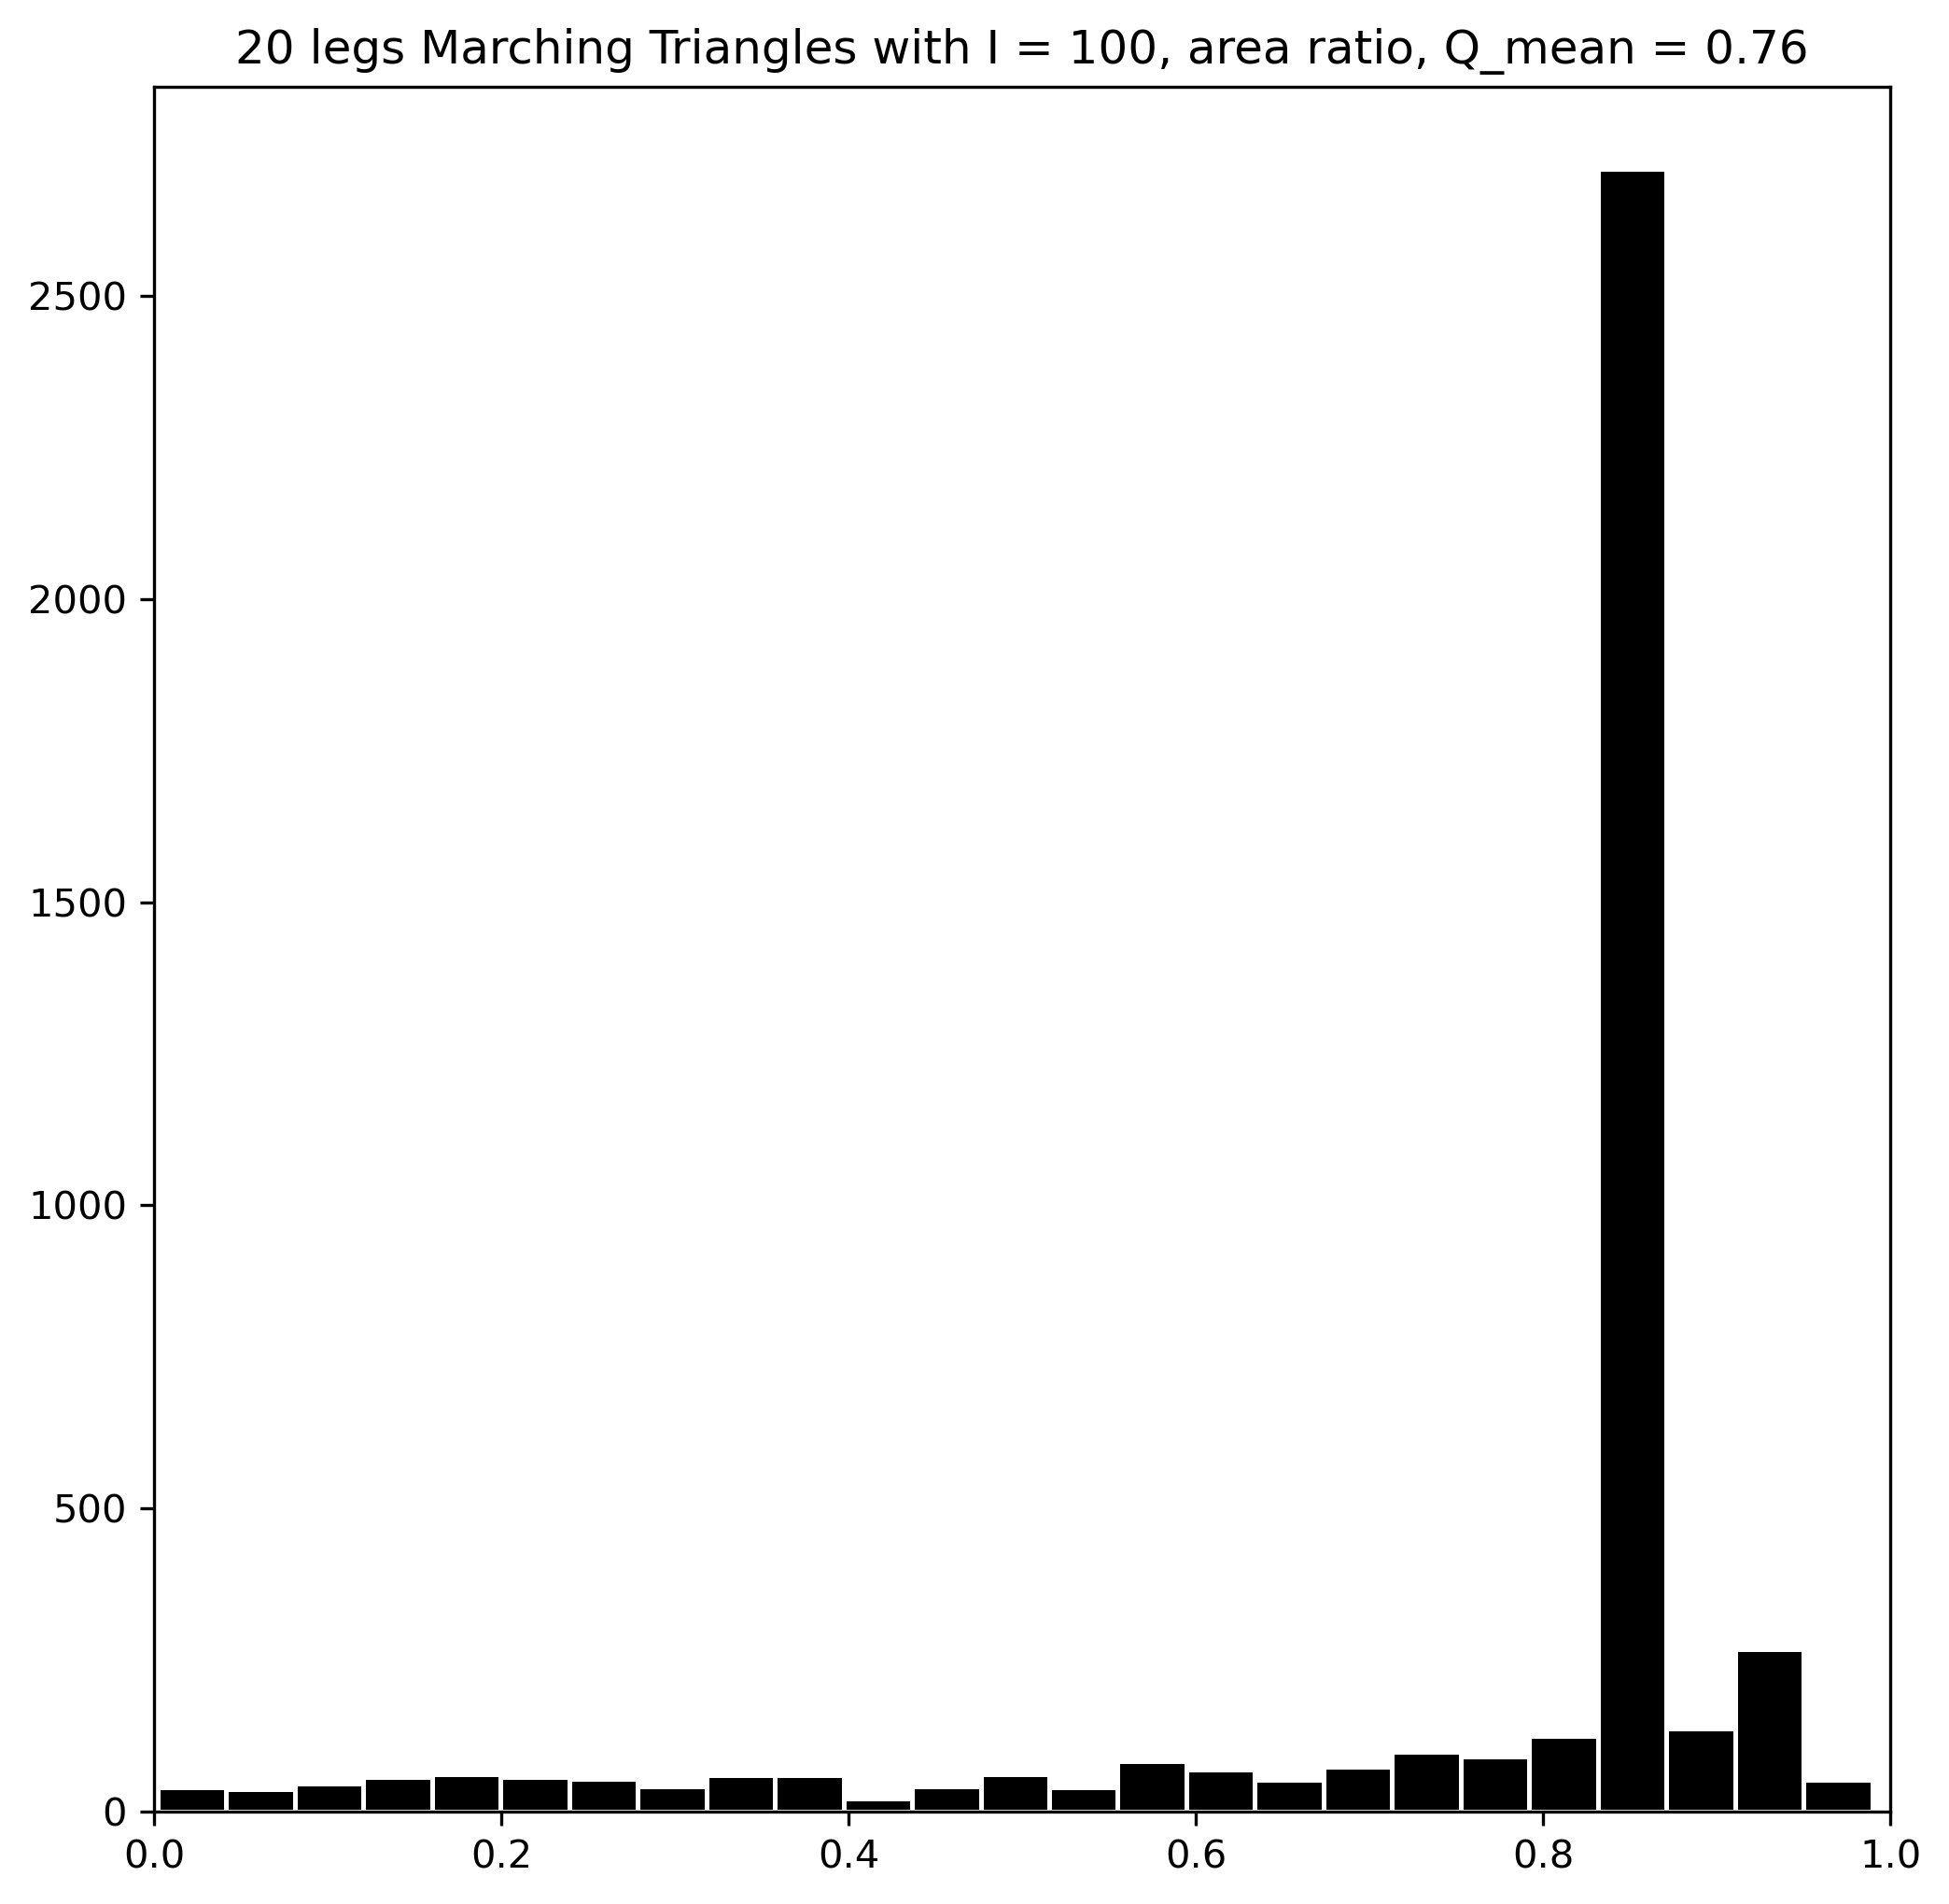
\includegraphics[width=\textwidth]{Images/histograms/20 legs Marching Triangles with I = 100, area ratio.png}
  \end{subfigure}
  \caption{Histograms of the radius and area ratios for the 5-legged and 20-legged star shape meshes generated with our marching traingles algorithm with grid sizes $I = 100$.
    We see that our marching triangles algorithm favors a specific type of triangle,
    which makes sense since we initially constructed them on a very regular, square grid.
    Another observation is that the amount of triangles deviating from this prioritized triangle is much higher for the 20-legged star.
    This happens because the ratio of boundary length to volume is much bigger here, and thus more triangles have to be altered by our algorithm,
    which results in them being of different qualities than the ones not altered by the algorithm.
    Note that we haven't included quality measures in the case of the grid size $I = 35$,
    since the 20-legged star broke down completely in this scenario, and thus proper comparison isn't possible.}
\end{figure}

\begin{figure}[H]
  \centering
  \begin{subfigure}{0.22\textwidth}
    \centering
    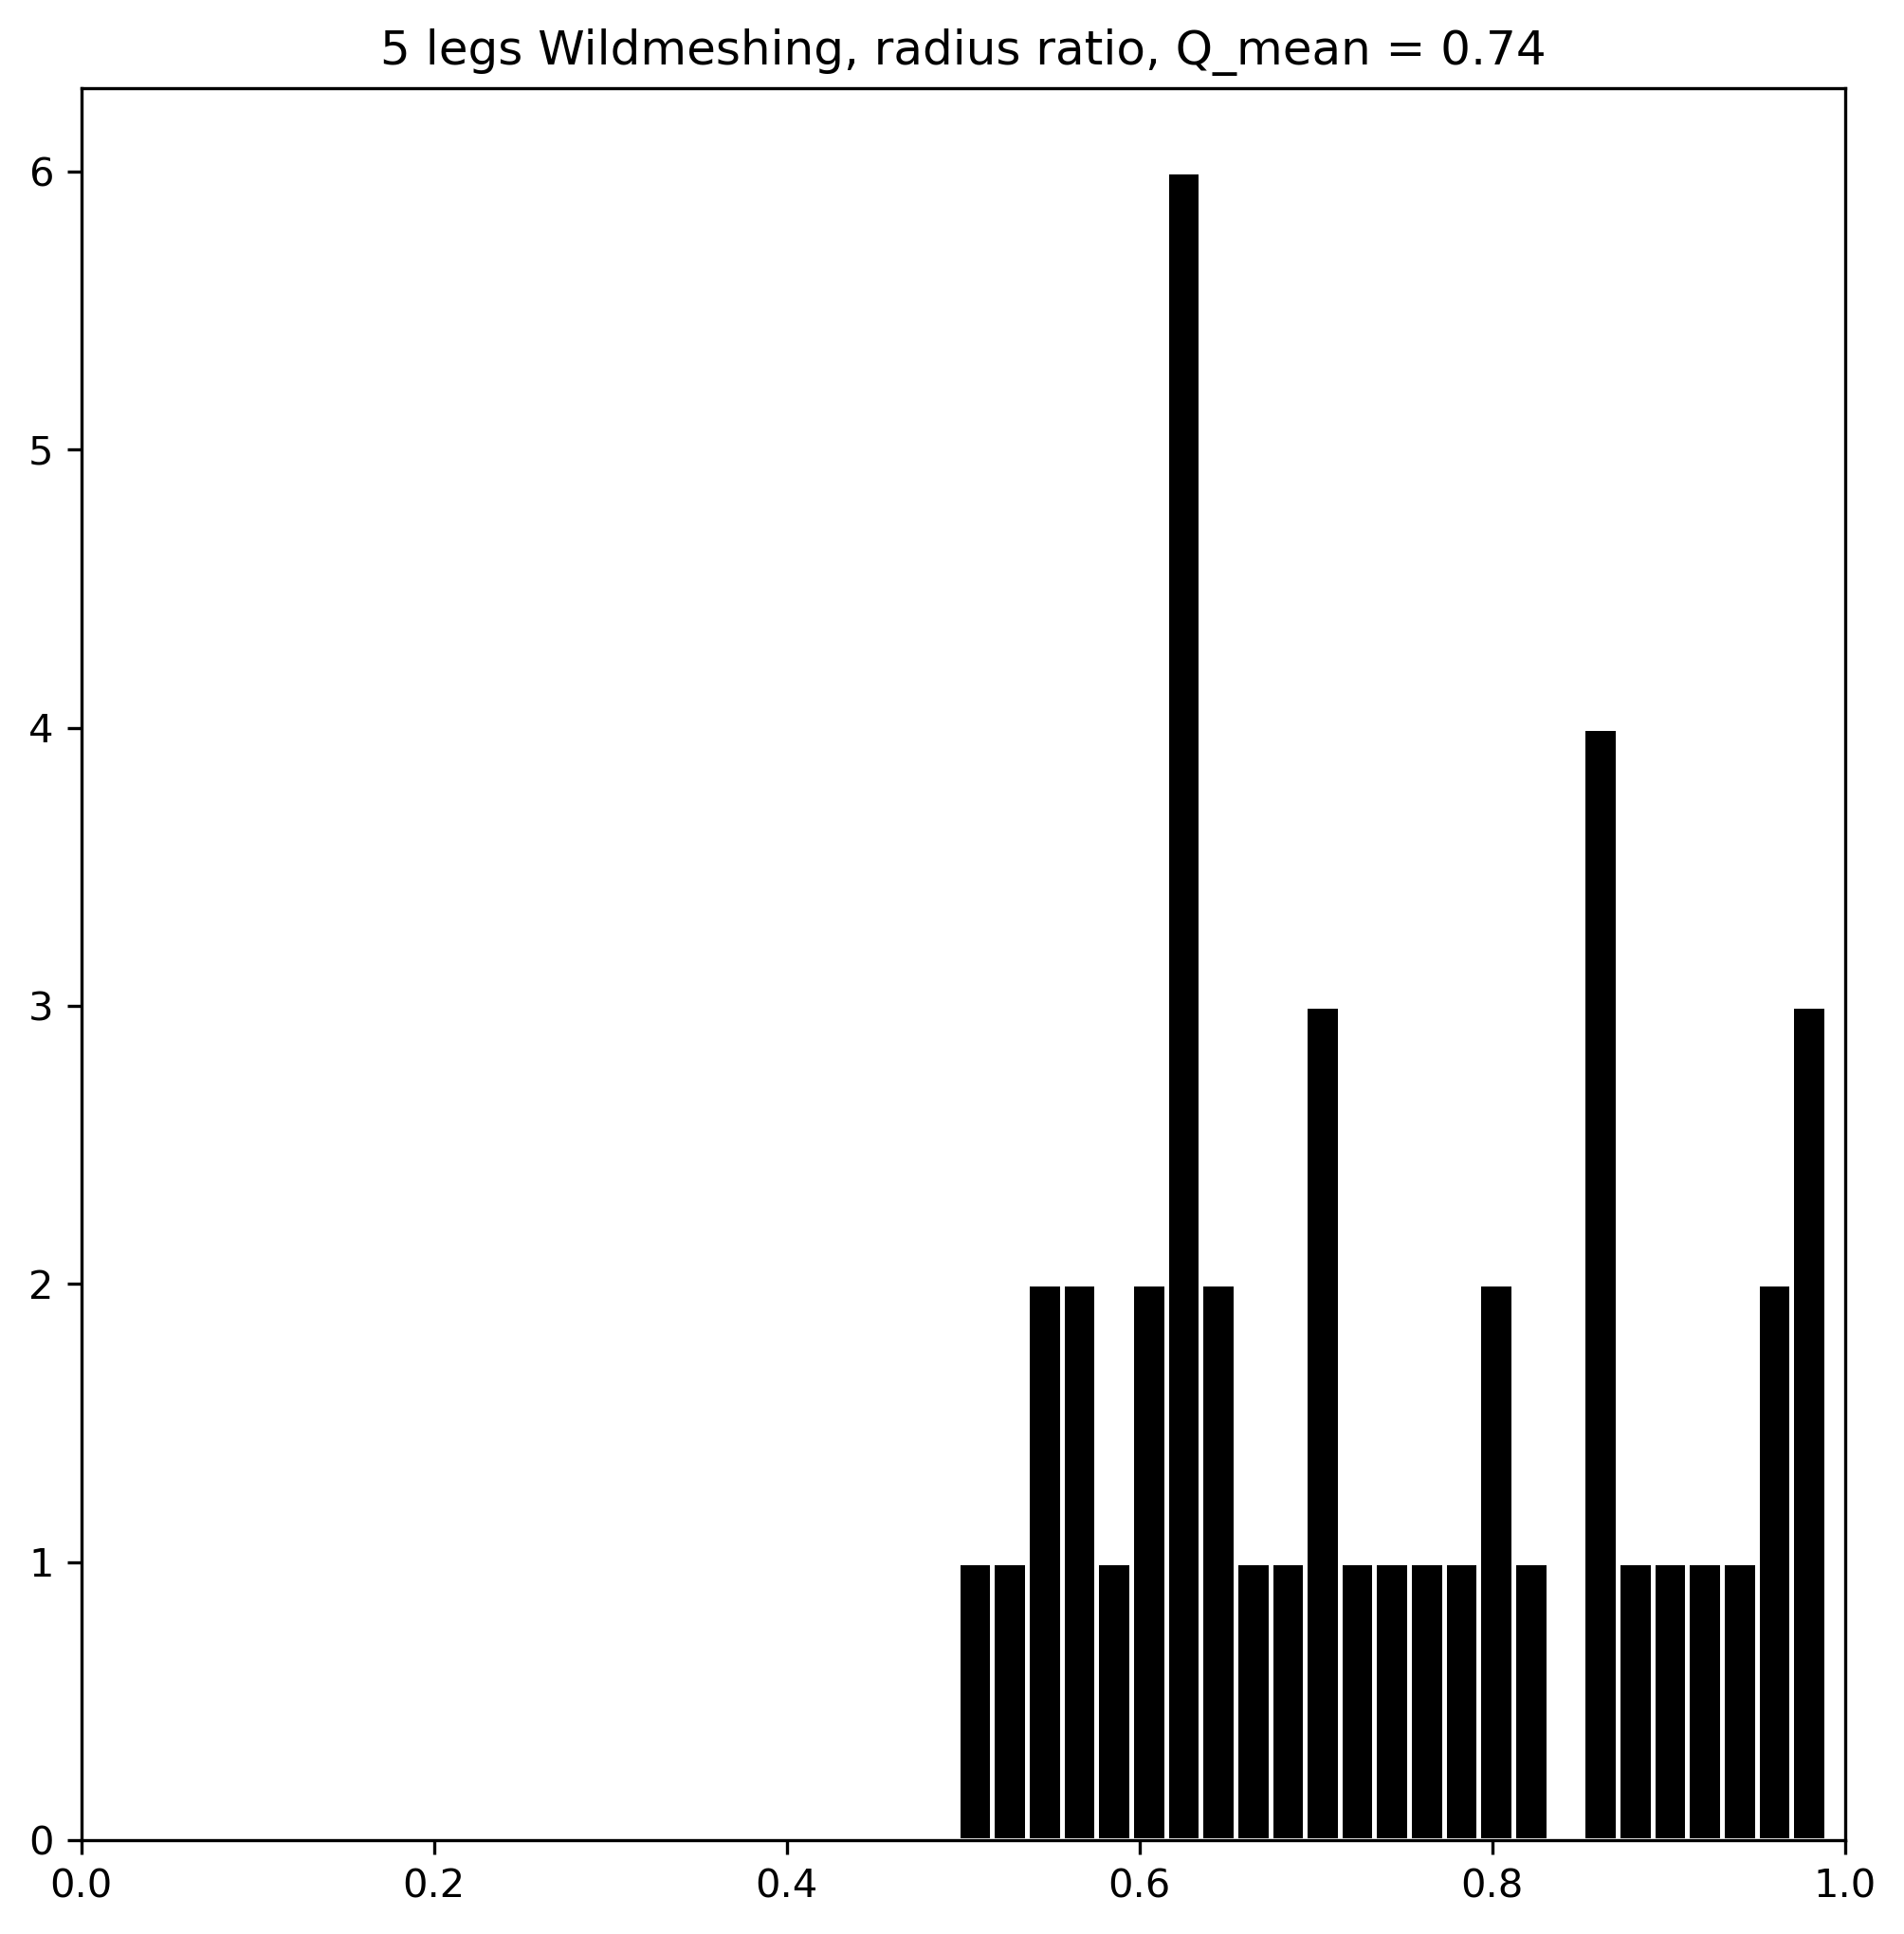
\includegraphics[width=\textwidth]{Images/histograms/5 legs Wildmeshing, radius ratio .png}
  \end{subfigure}\hfill
  \begin{subfigure}{0.22\textwidth}
    \centering
    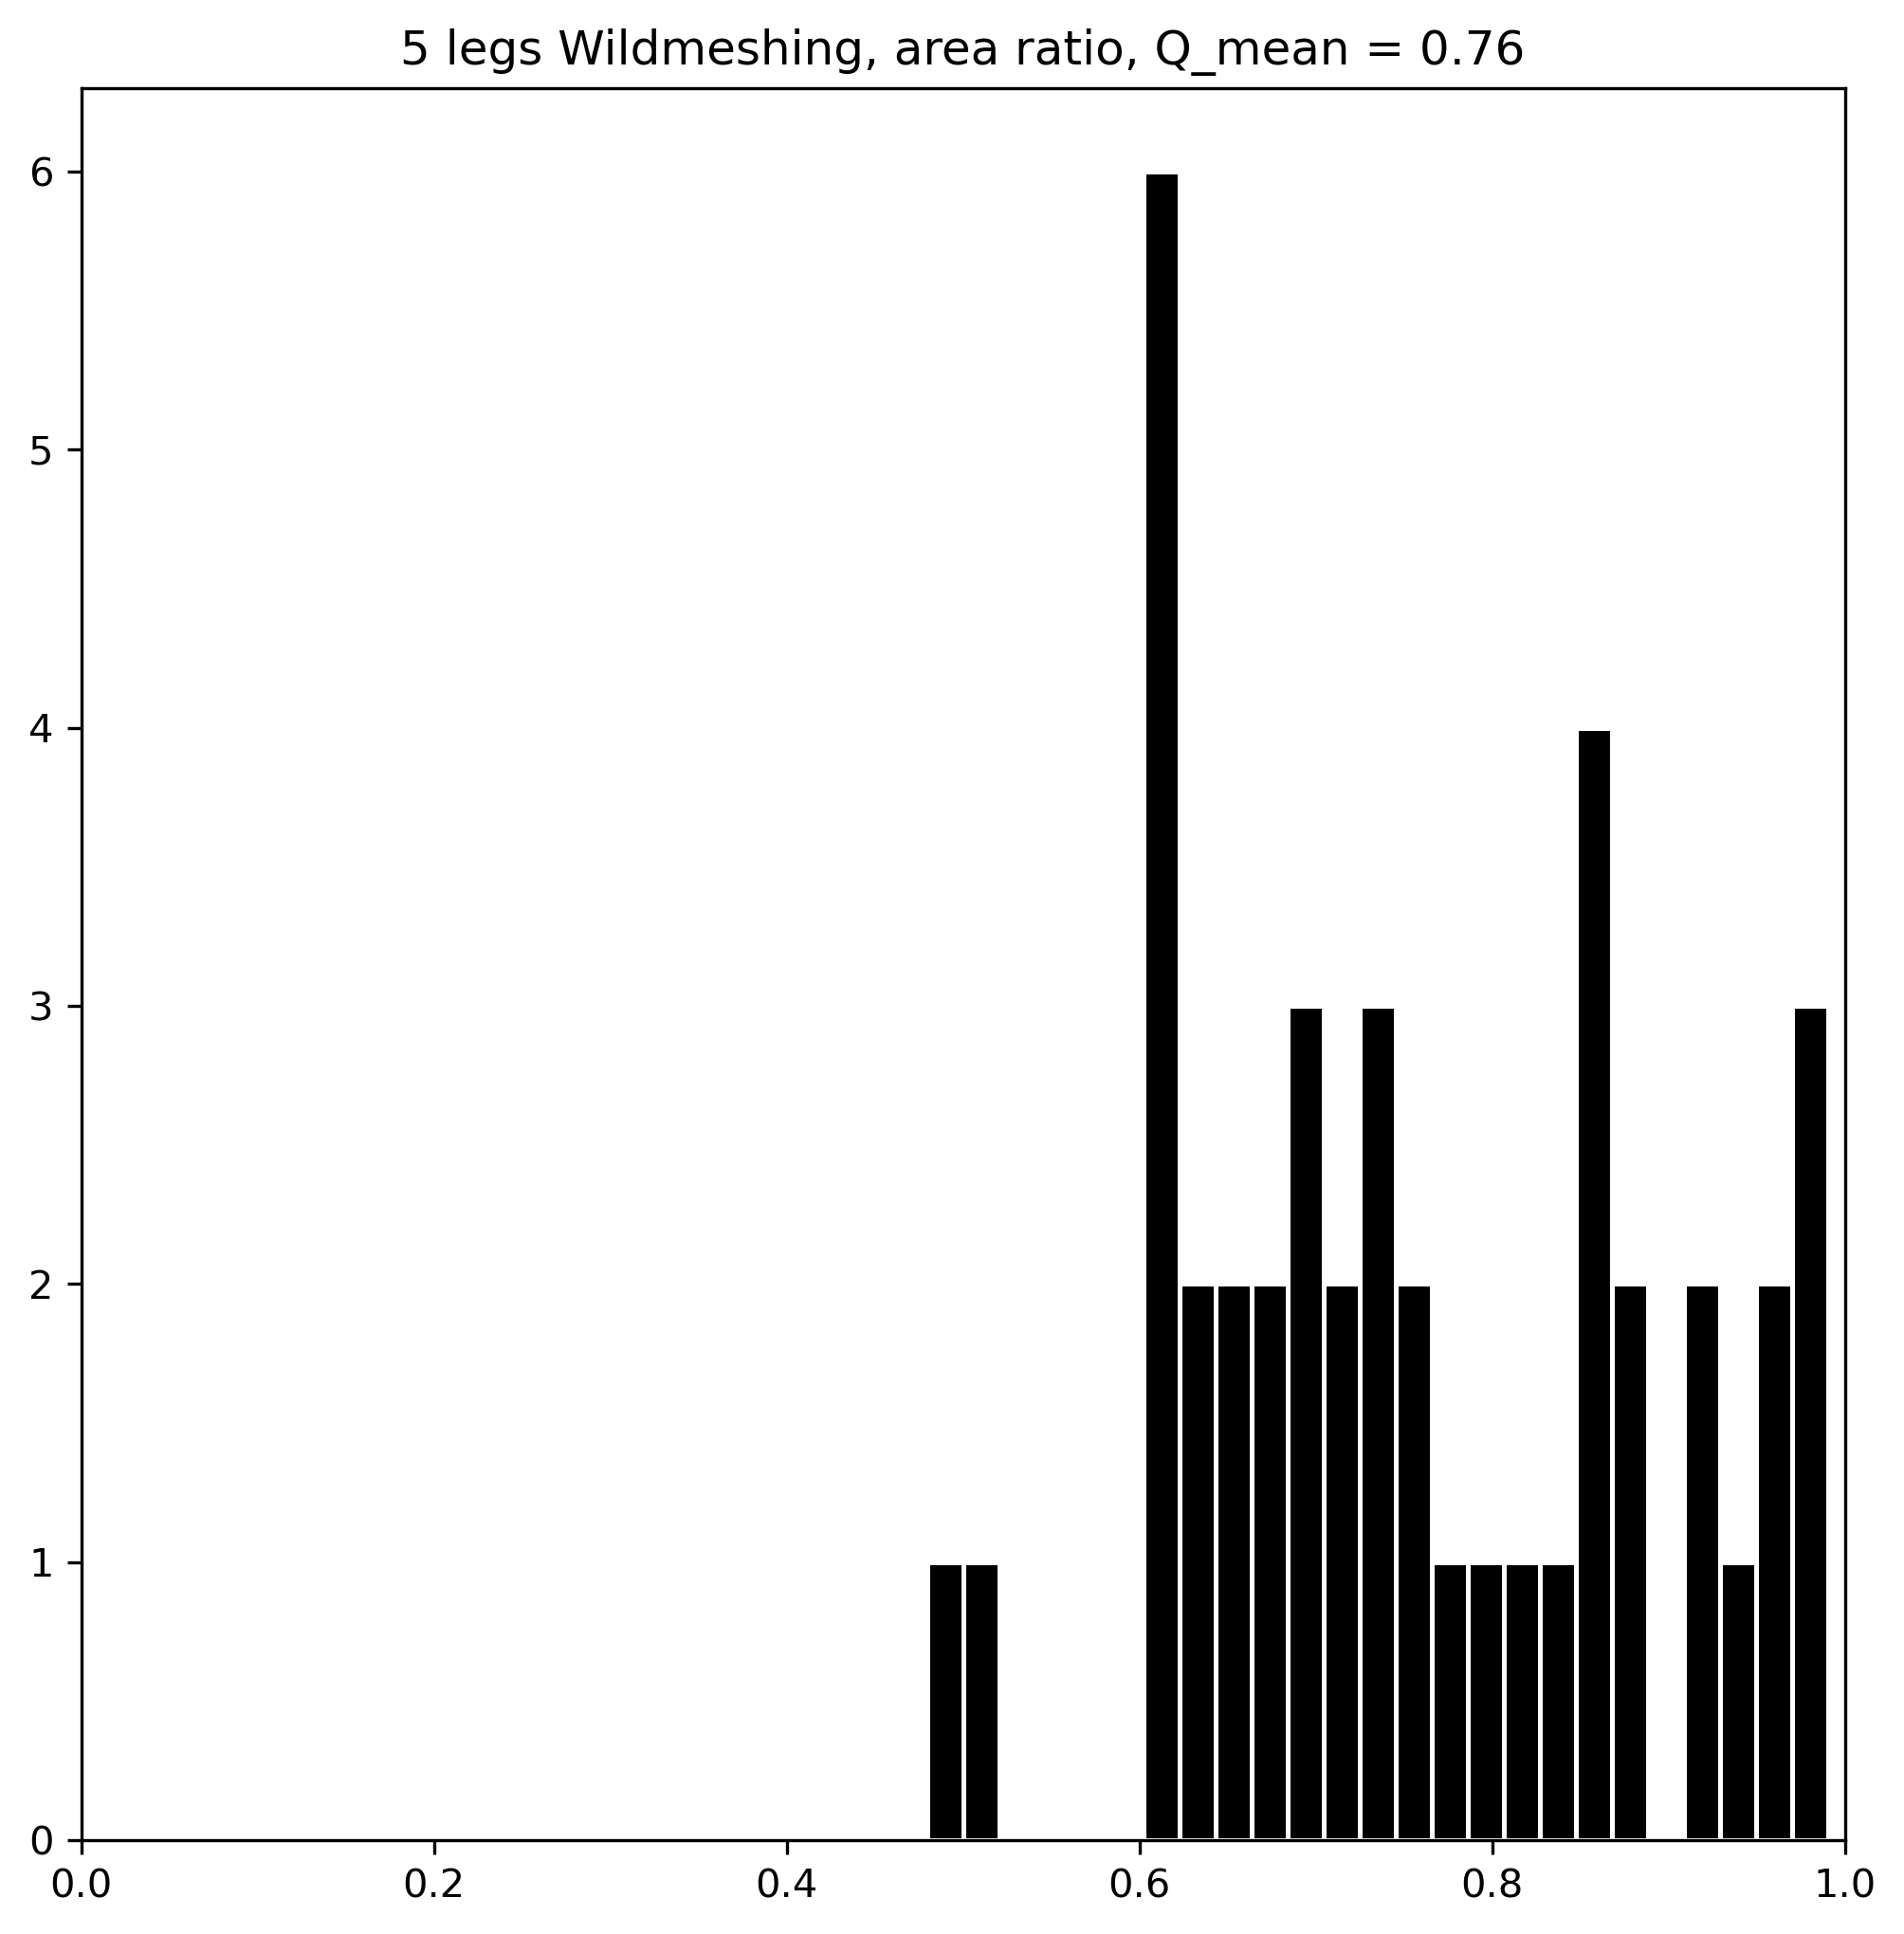
\includegraphics[width=\textwidth]{Images/histograms/5 legs Wildmeshing, area ratio .png}
  \end{subfigure}
  \begin{subfigure}{0.22\textwidth}
    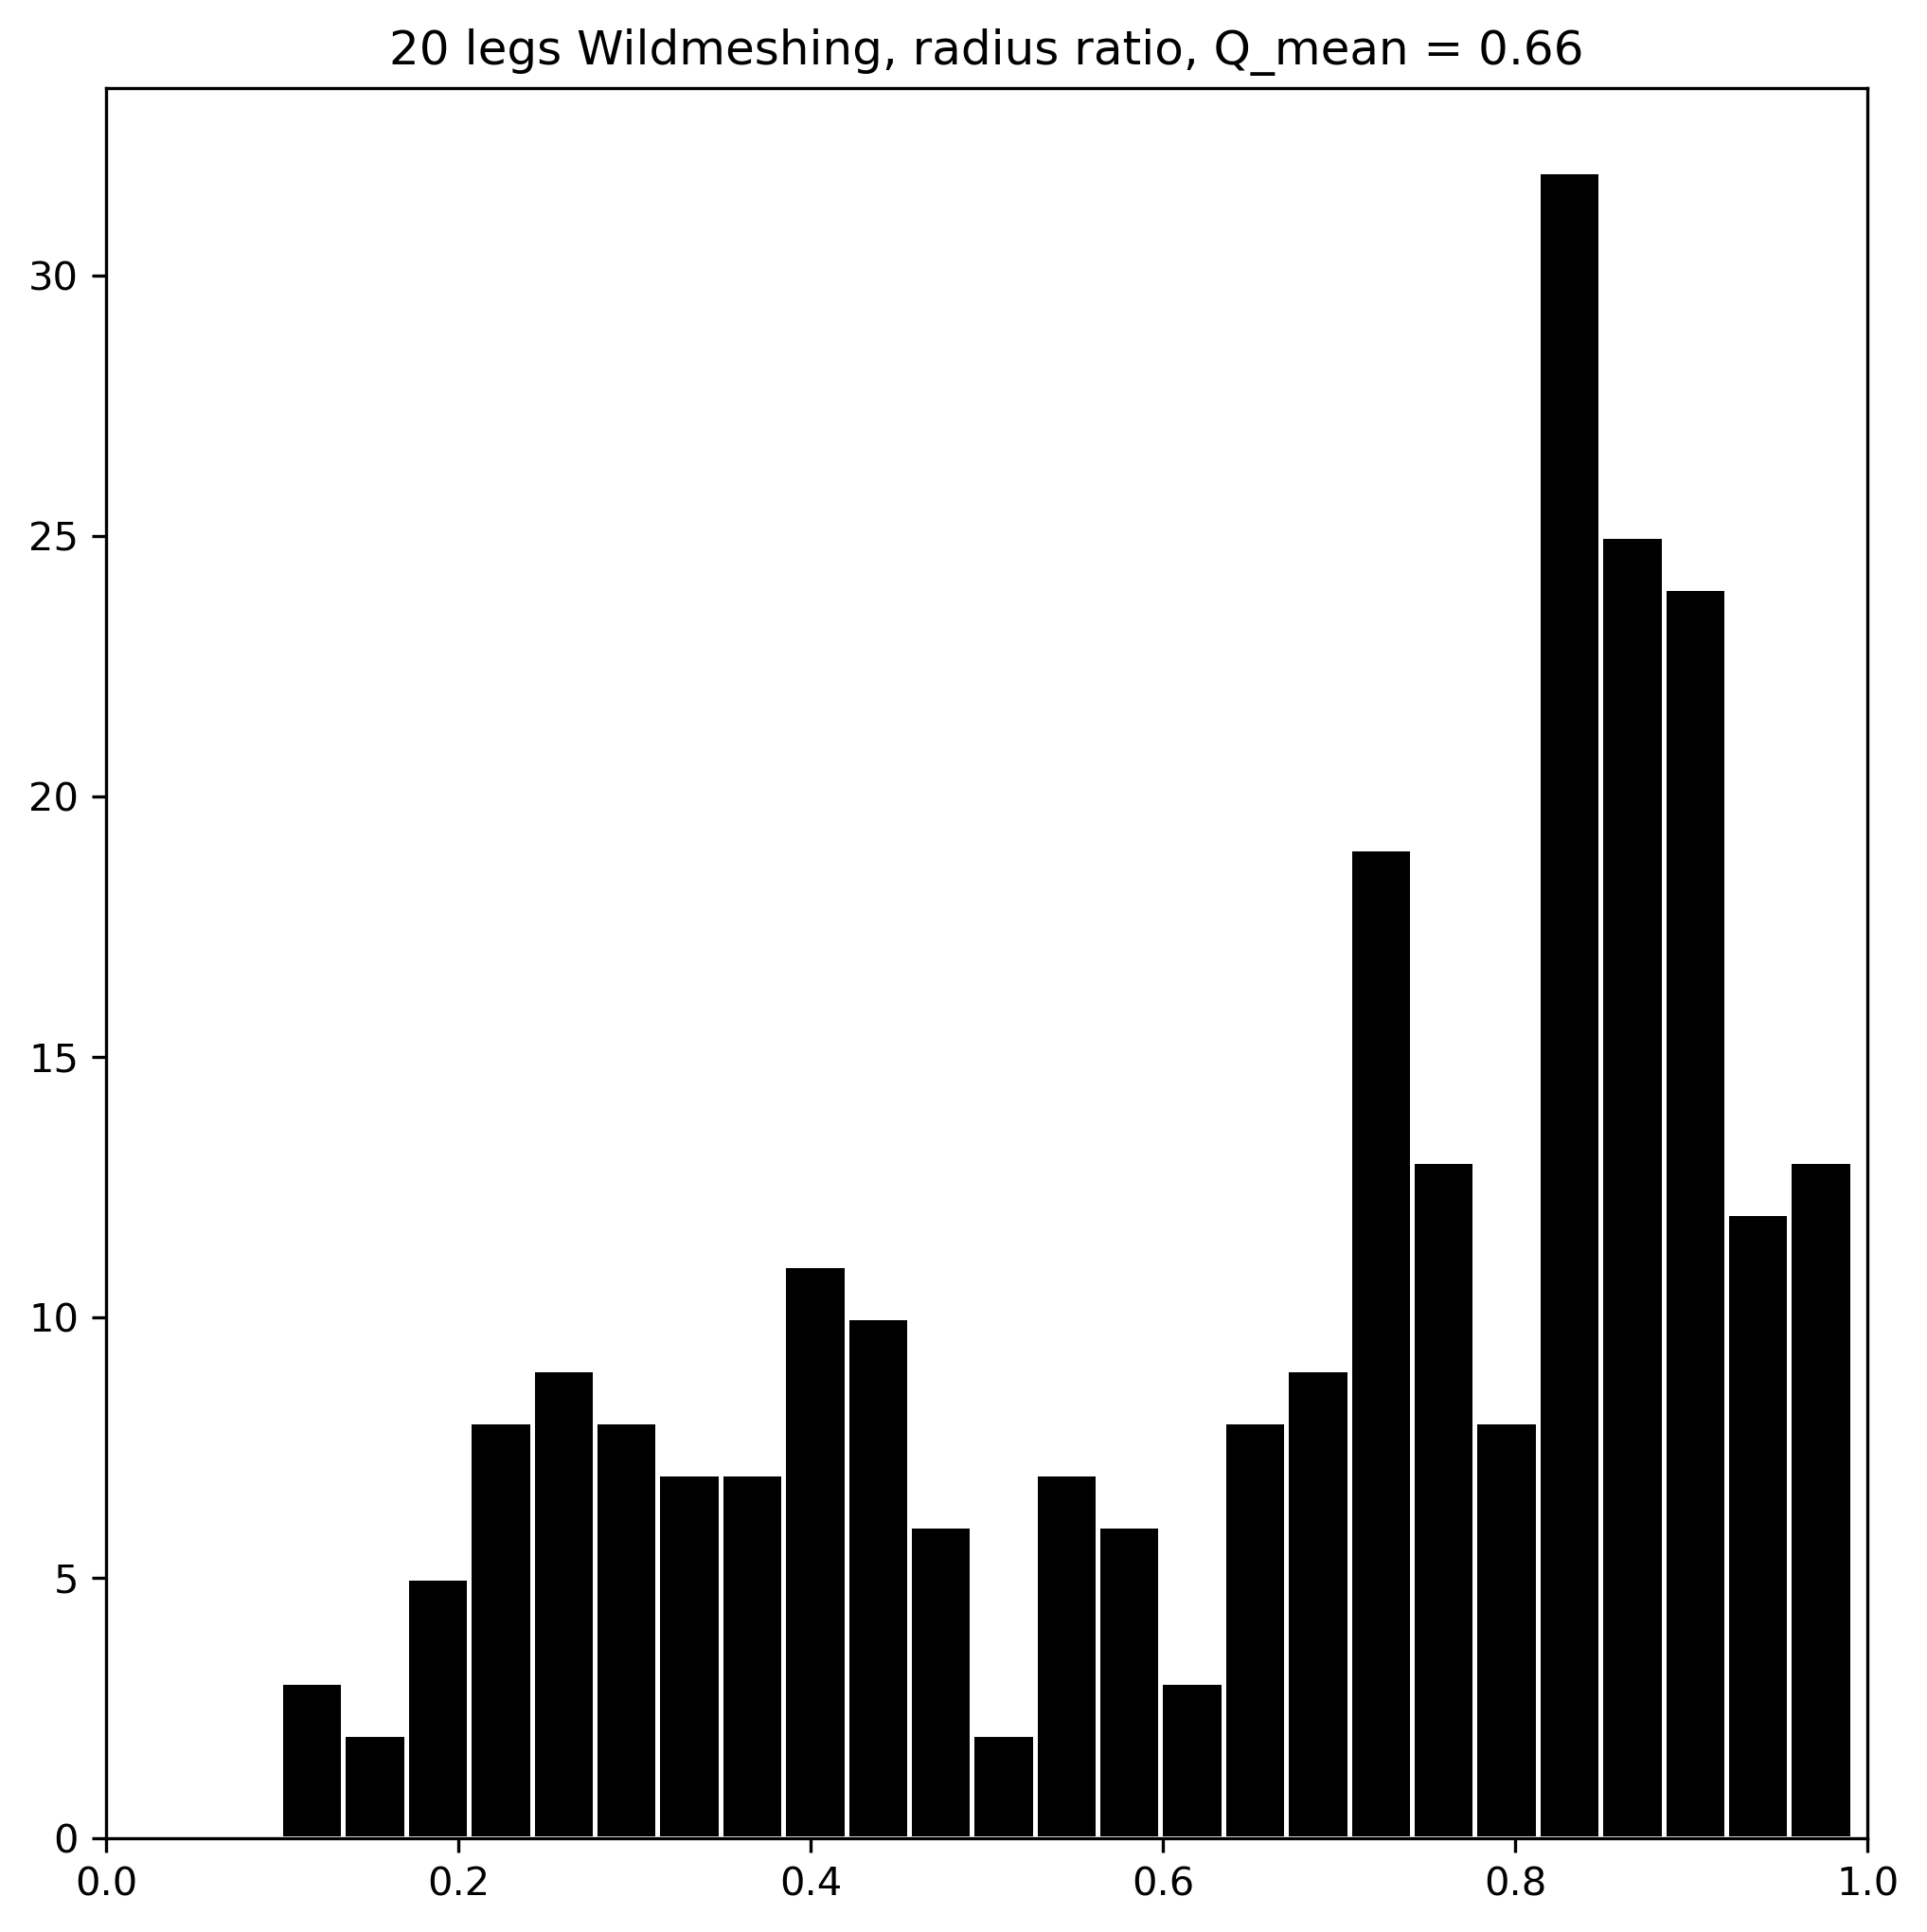
\includegraphics[width=\textwidth]{Images/histograms/20 legs Wildmeshing, radius ratio .png}
    \centering
  \end{subfigure}\hfill
  \begin{subfigure}{0.22\textwidth}
    \centering
    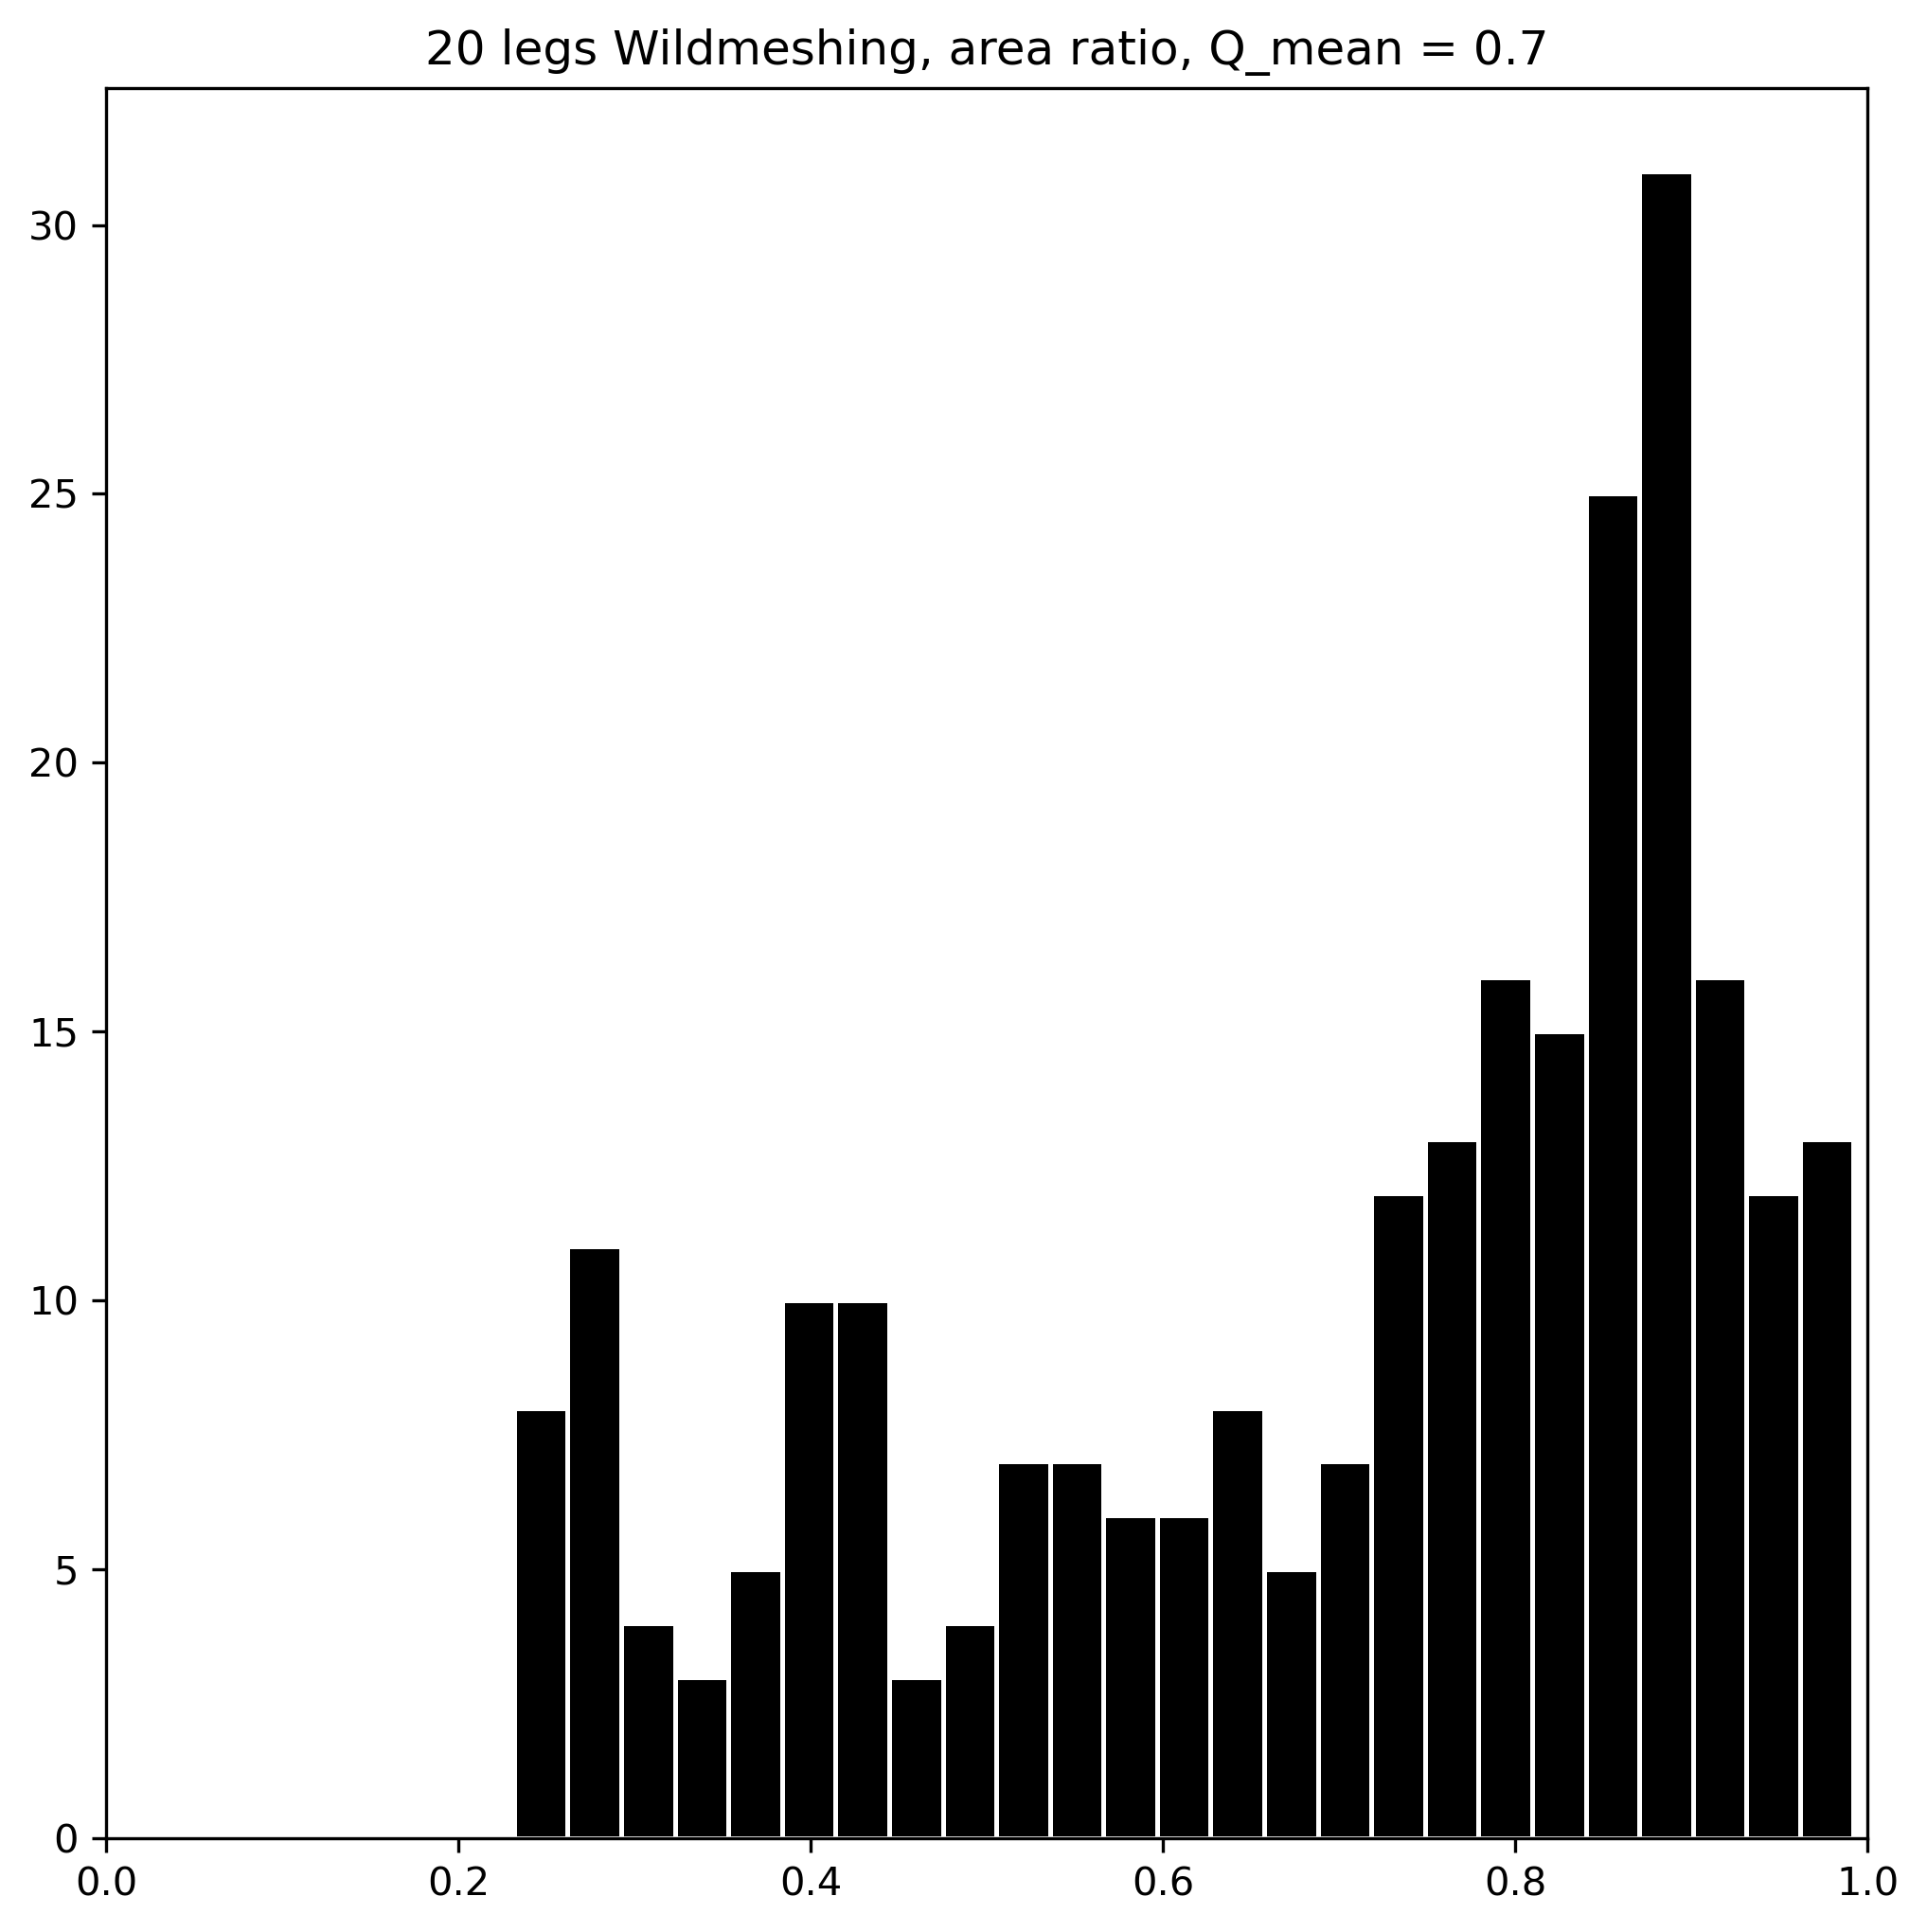
\includegraphics[width=\textwidth]{Images/histograms/20 legs Wildmeshing, area ratio .png}
  \end{subfigure}
  \caption{Histograms of the radius and area ratios for the 20-legged star shape meshes generated with the Wildmeshing algorithm.
    We see that in the case of the 5-legged star, the Wildmeshing algorithm generates only a few triangles,
    and thus, their histograms have very low statistics, but in general the quality of the triangles generated is above 0.5.
    For the 20-legged star, way more triangles were generated, and we see that their qualities are pretty uniformly distributed with a slight trend towards around 0.9.
    Seen in this light, it seems that teh quality of our algorithm is actually better than the Wildmeshing algorithm,
    but this is probably not the case. The reason is, that we have a very high concentration of low quality triangles
    around all of the boundary of the shape, and very different quality triangles on the inside, which could cause inconsistencies when simulating.}
\end{figure}

\begin{figure}[H]
  \centering
  \begin{subfigure}{0.22\textwidth}
    \centering
    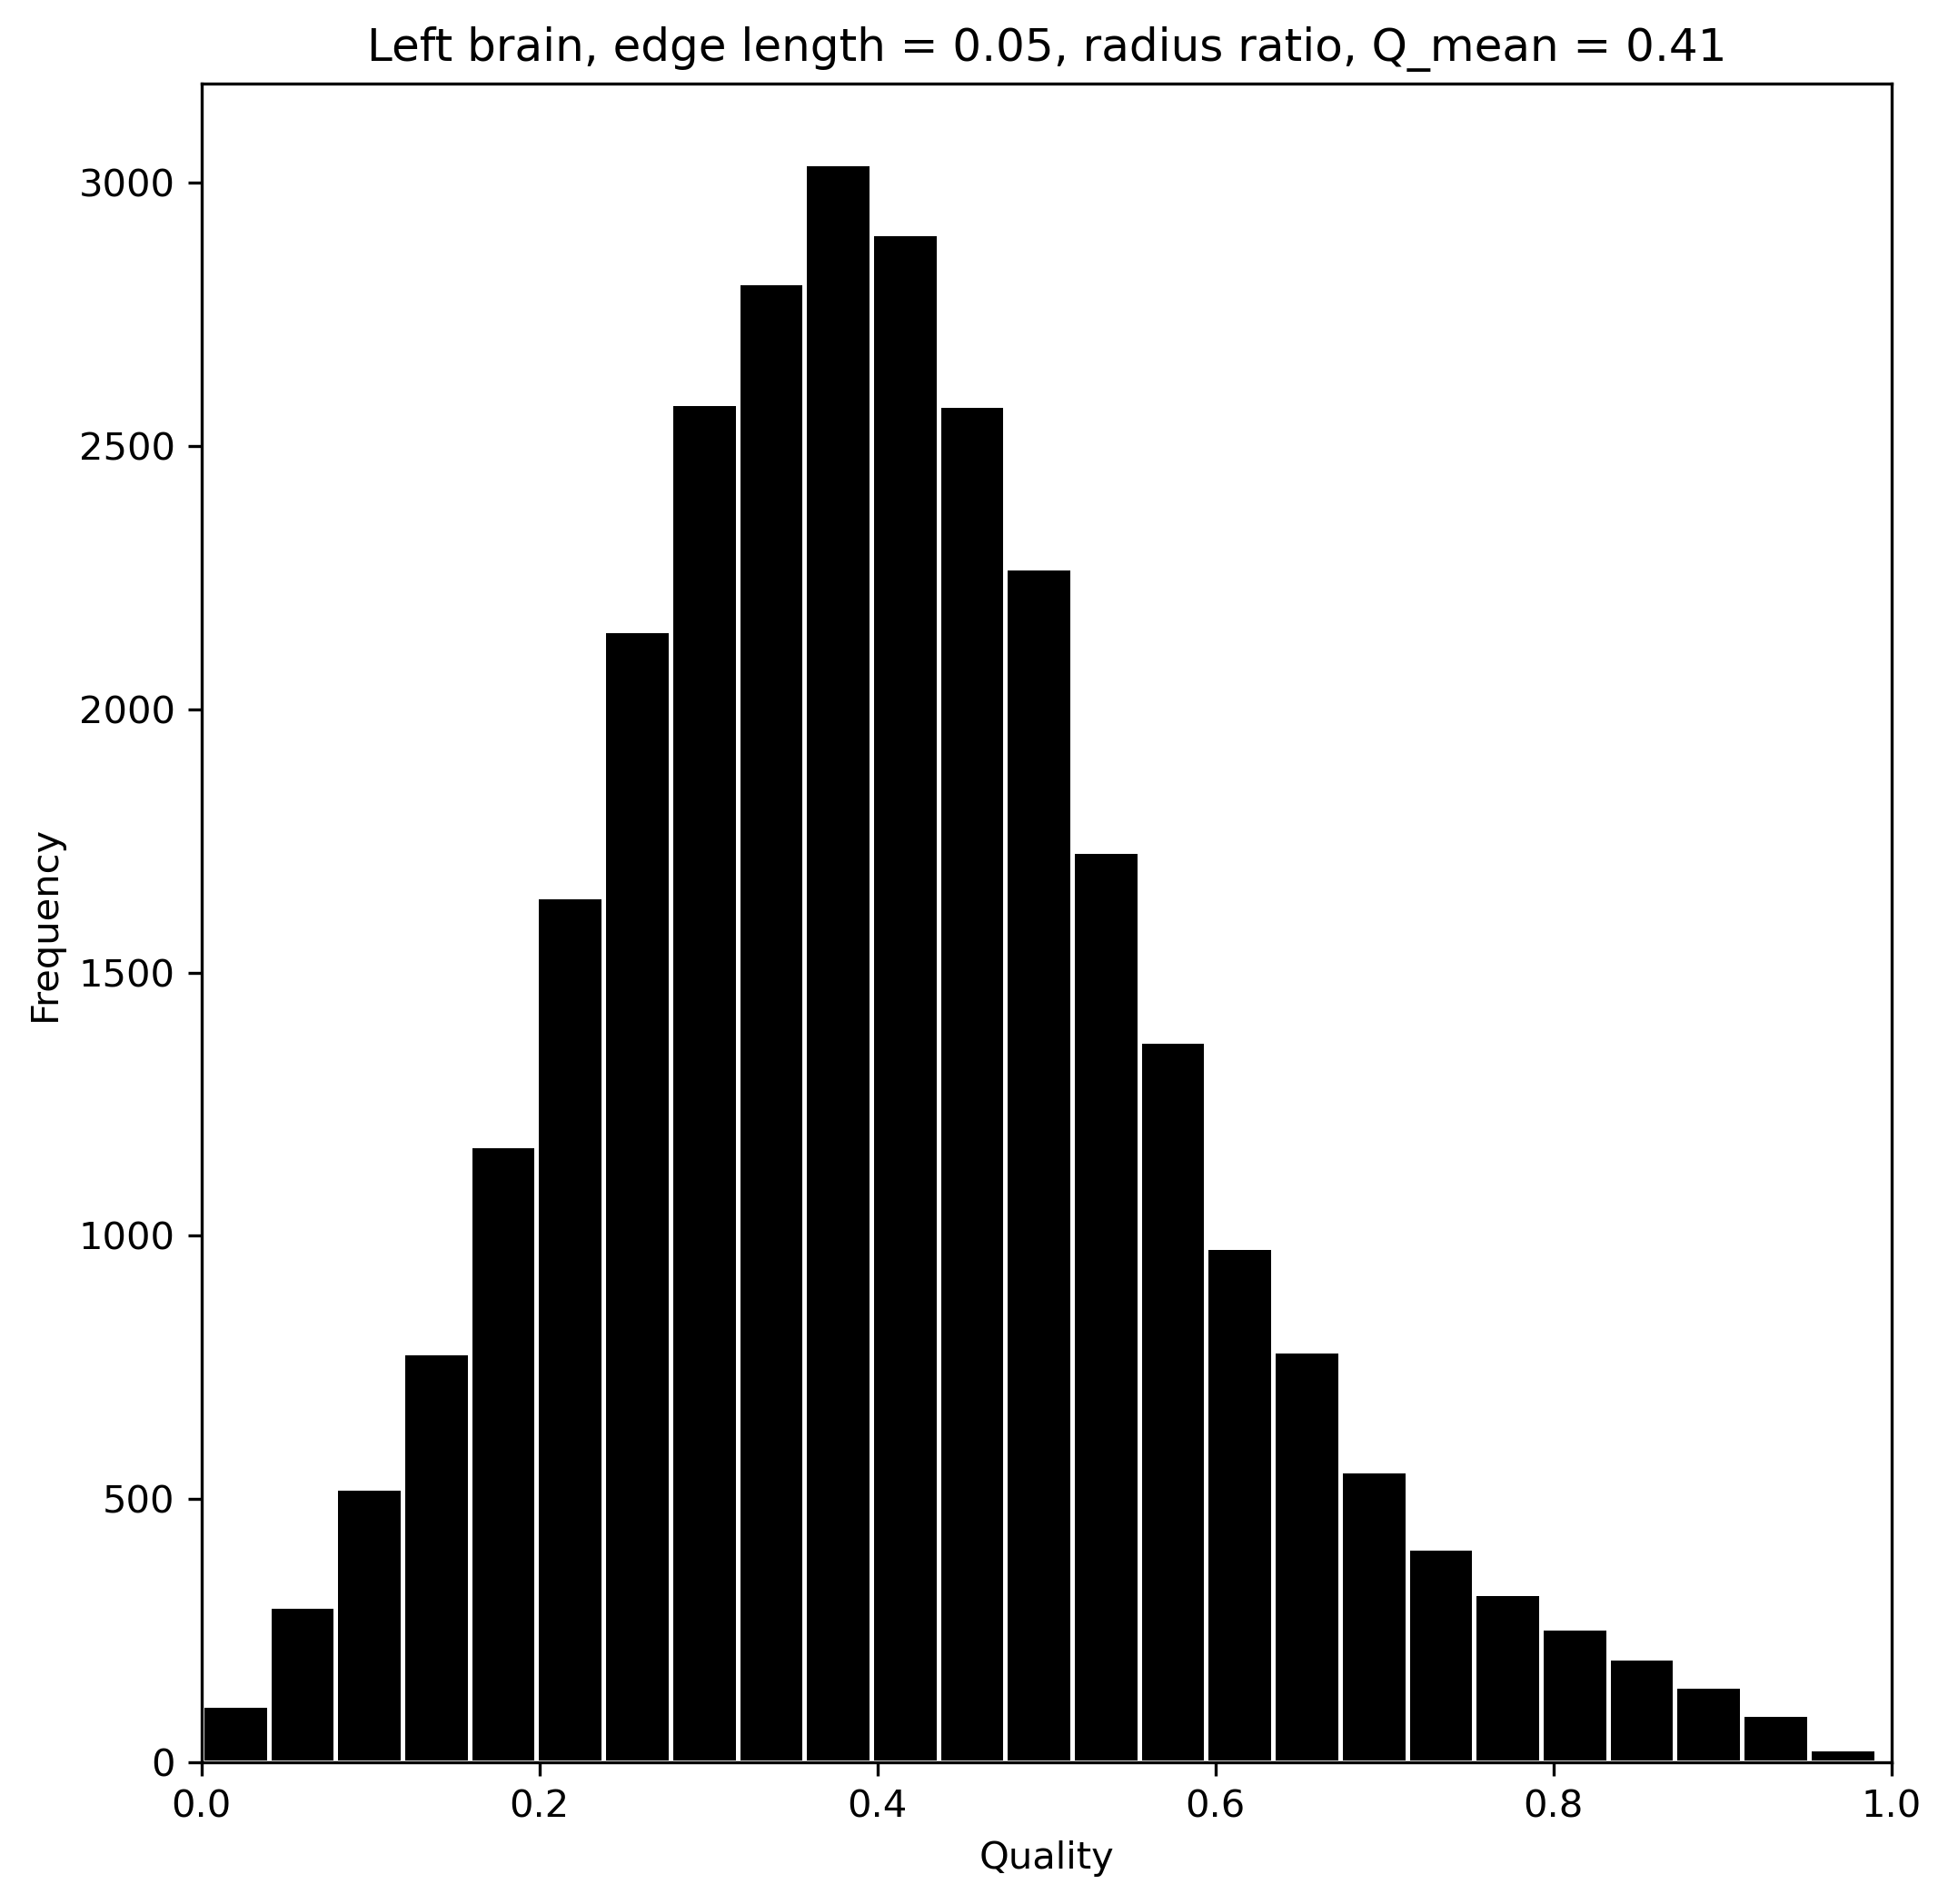
\includegraphics[width=\textwidth]{Images/histograms/Left brain, edge length = 0.05, radius ratio.png}
  \end{subfigure}\hfill
  \begin{subfigure}{0.22\textwidth}
    \centering
    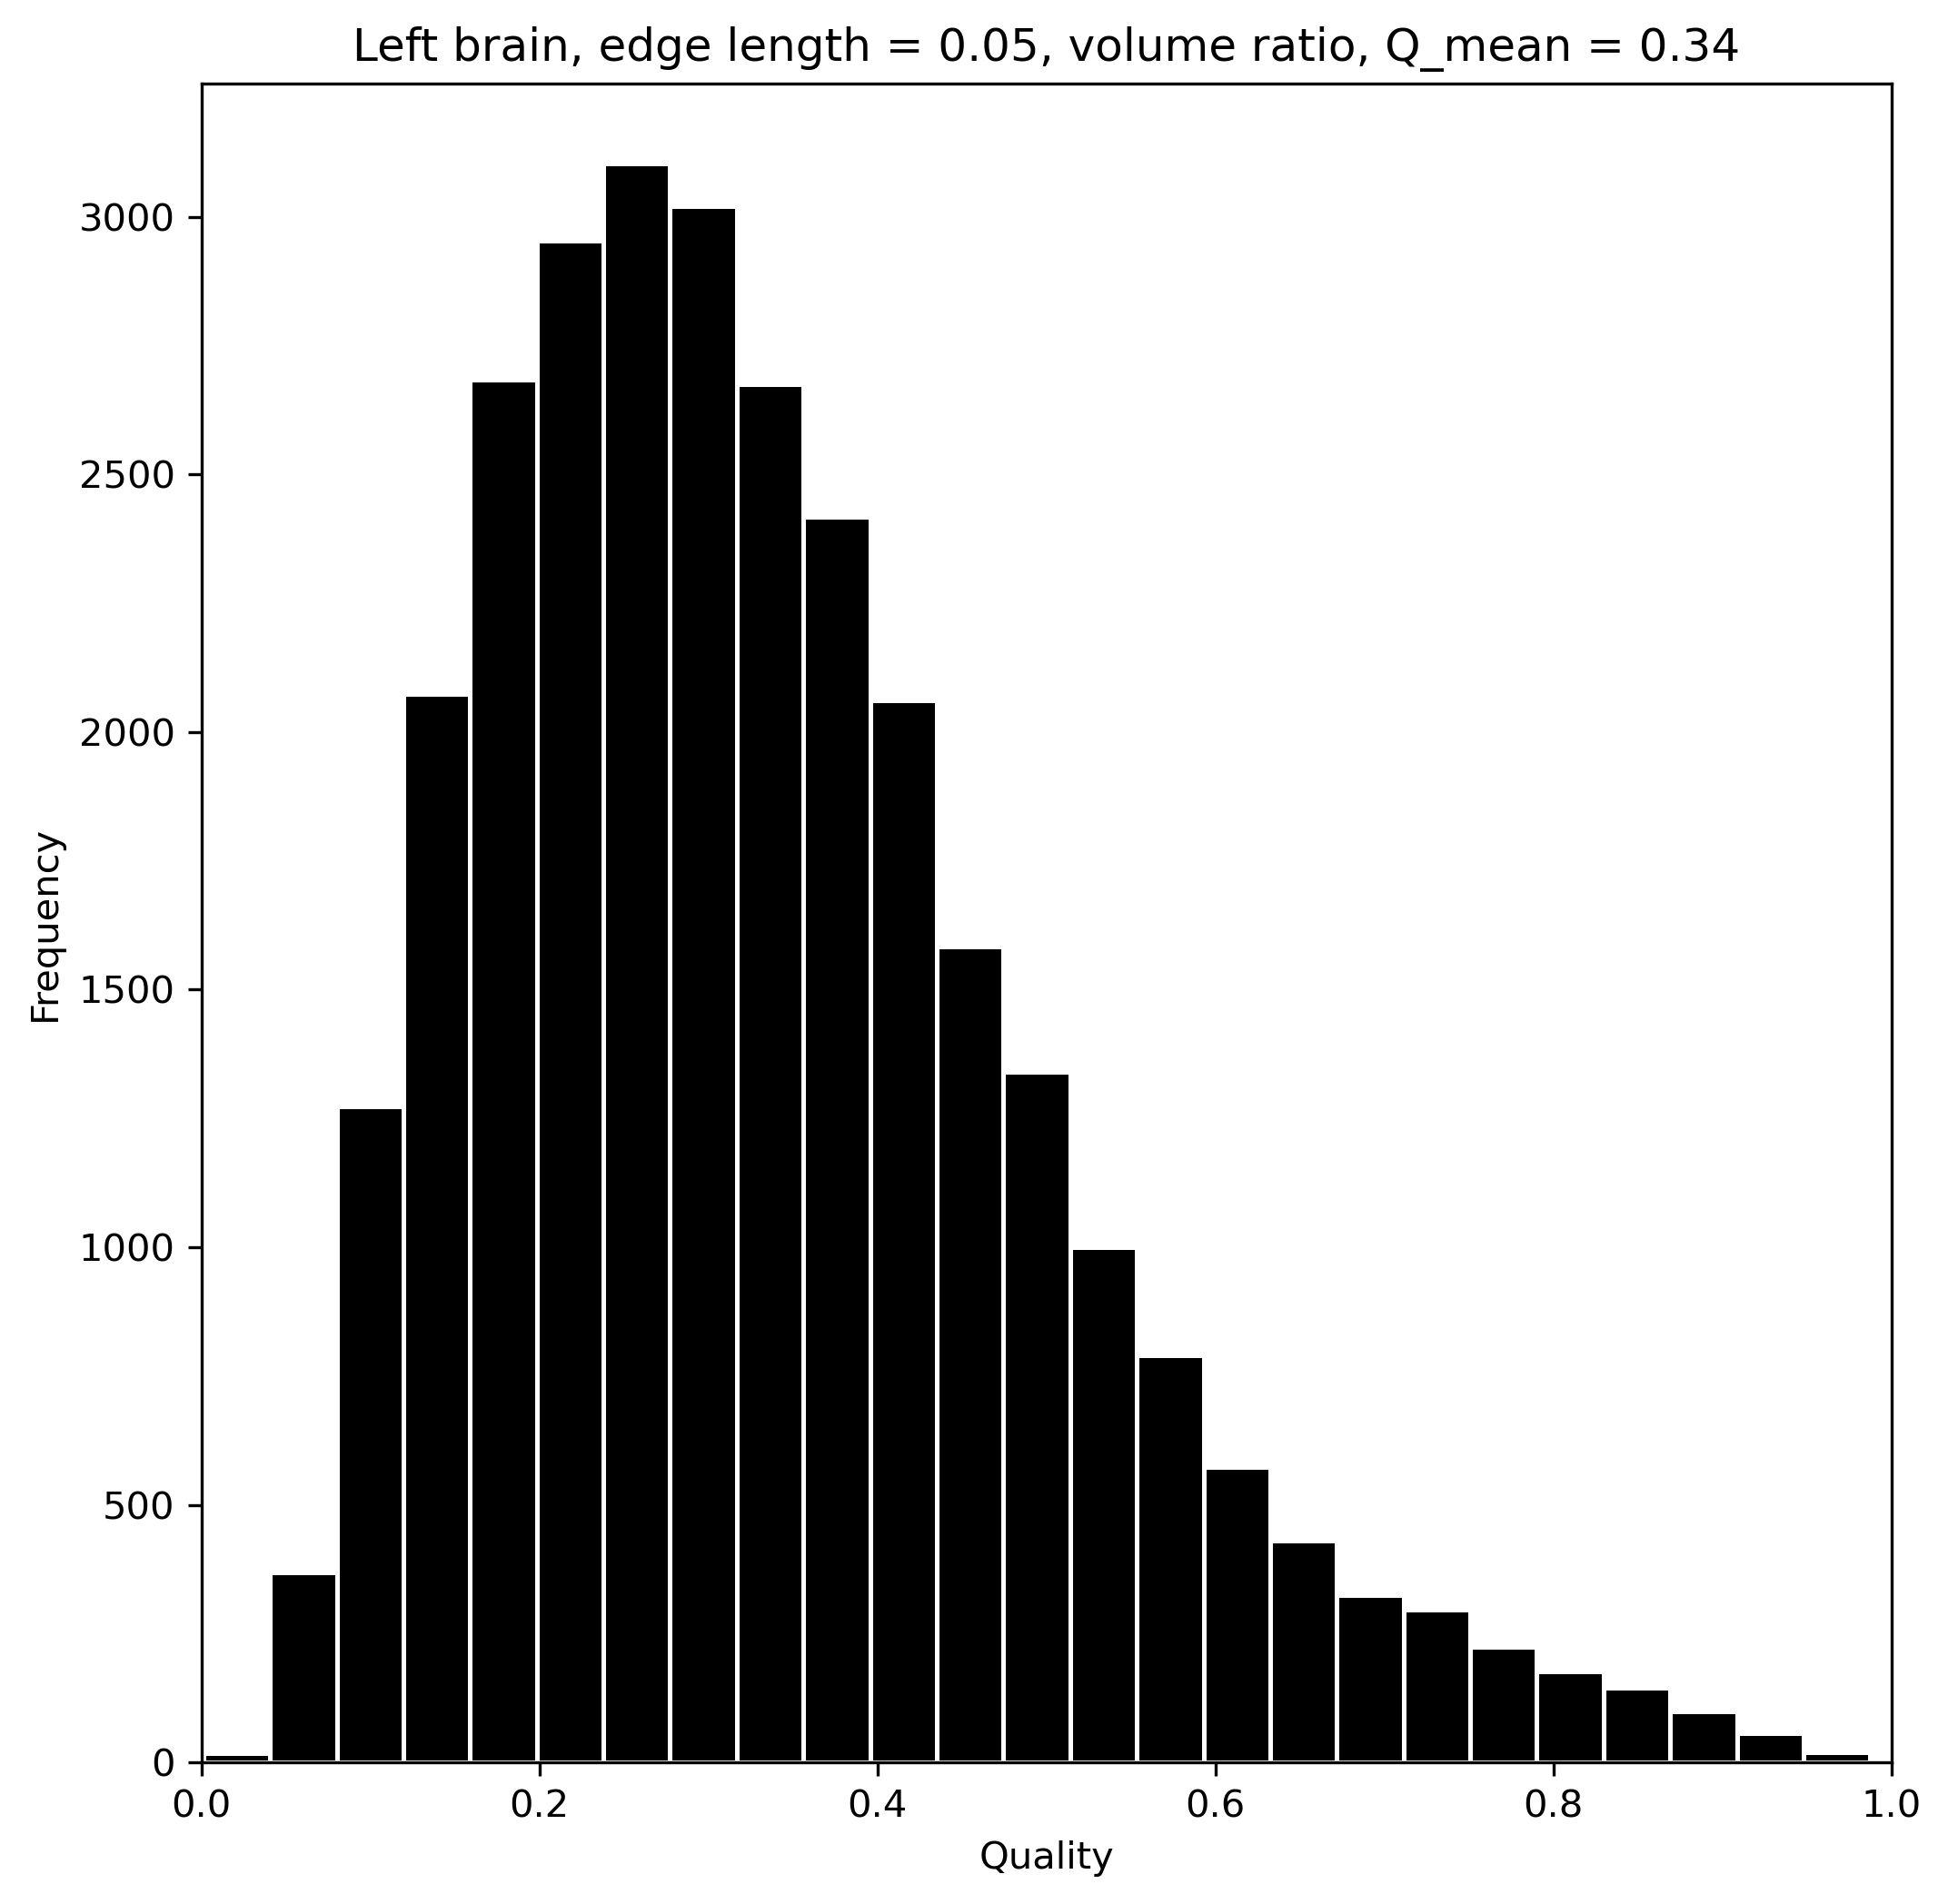
\includegraphics[width=\textwidth]{Images/histograms/Left brain, edge length = 0.05, volume ratio.png}
  \end{subfigure}
  \begin{subfigure}{0.22\textwidth}
    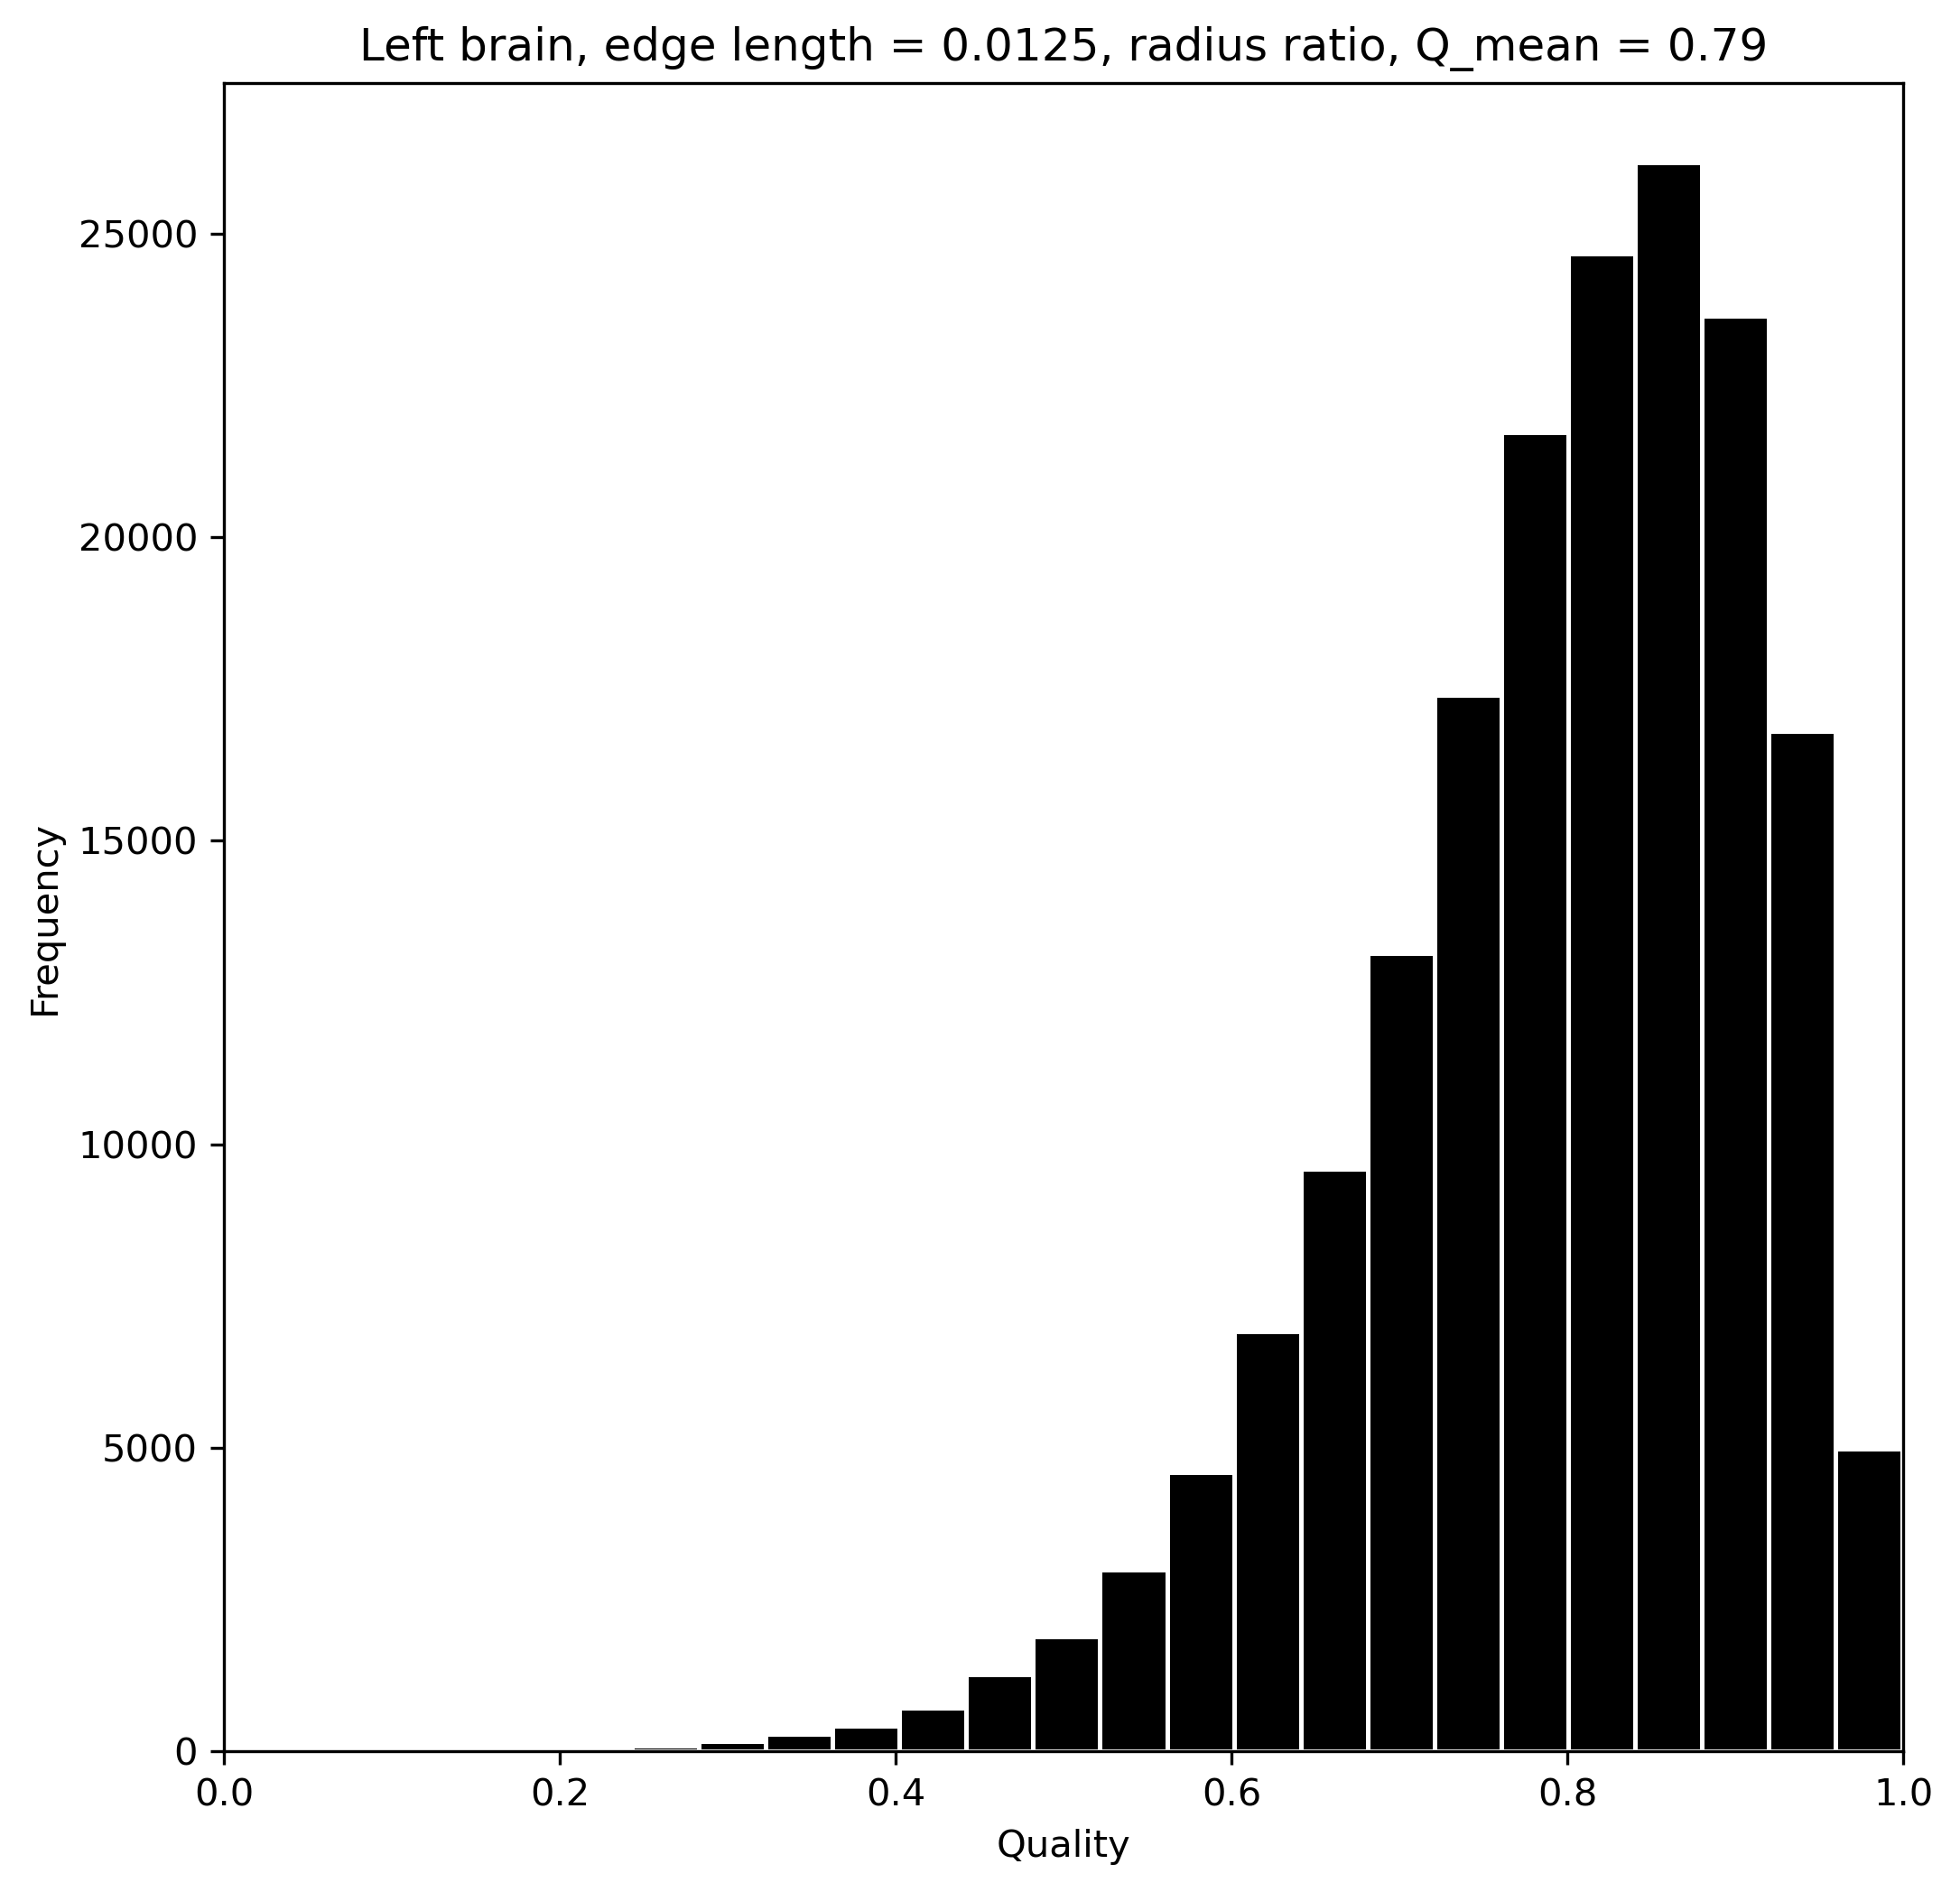
\includegraphics[width=\textwidth]{Images/histograms/Left brain, edge length = 0.0125, radius ratio.png}
    \centering
  \end{subfigure}\hfill
  \begin{subfigure}{0.22\textwidth}
    \centering
    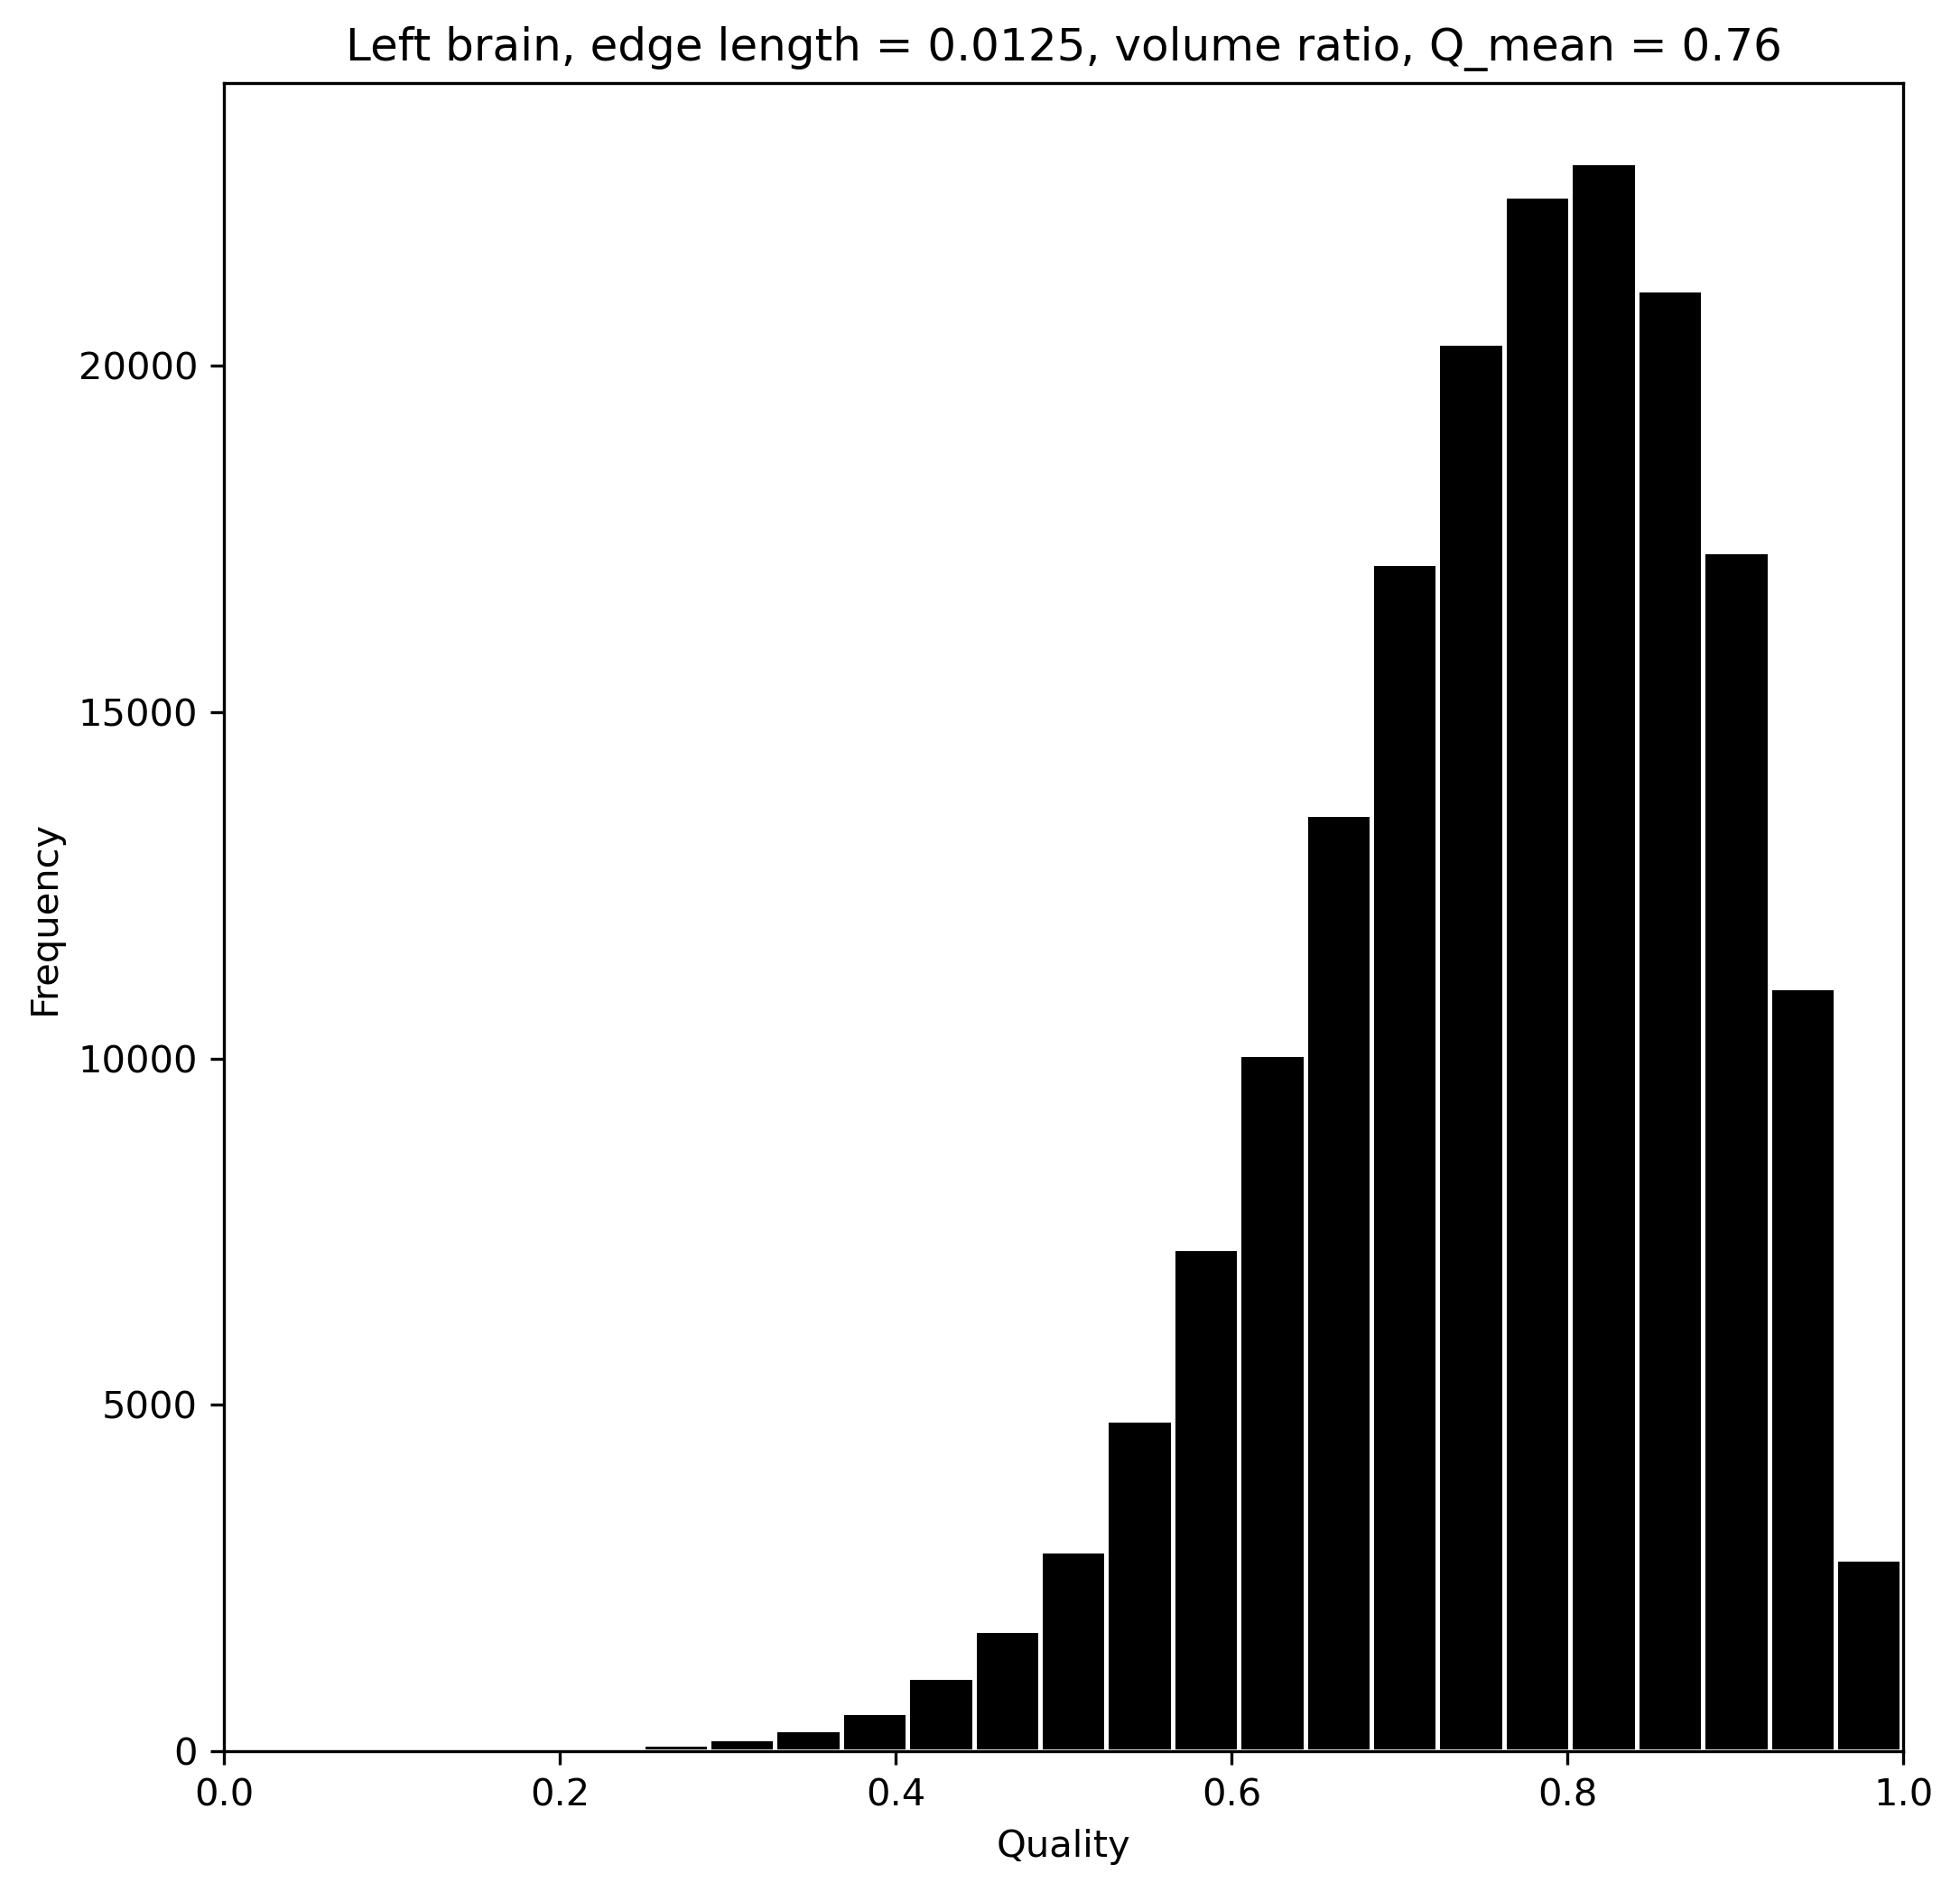
\includegraphics[width=\textwidth]{Images/histograms/Left brain, edge length = 0.0125, volume ratio.png}
  \end{subfigure}
  \caption{Histograms of the radius and area ratios for the tetrahedral mesh of the left brain model generated by the Wildmeshing tetrahedralizer algorithm.
    The experiments were done with edge length settings $l_\mathrm{edge}  = 0.05$ and $l_\mathrm{edge}  = 0.0125$.
    We see that the hsitograms have very smooth distributions, centered around specific quality values.
    Importantly, we see, that the quality is greater for the finer edge length setting, which is expected.}
\end{figure}

\section{Conclusion}
After having looked at some different meshes in both 2D and 3D and analyzing
the quality distributions of their elements, we have a couple things that we
can conclude. Generally, finner grids are better at capturing the shape of the
polygon, but also increases the number of elements in the mesh. The marching
triangles algorithm results in a lot of very similar triangles and then few
very irregular triangles at the edges of the polygon. This causes assymetries
and inconsistencies in the mesh, which could cause problems when simulating,
since, on the inside of the domain, the mesh is of high quality, but, at the
boundary, it's of very poor quality. The Wildmeshing alogrithm generally yields
a drastically lower number of elements, with various quality measures that are
more smoothly distributed. This is probably due to the fact that the
Wildmeshing algorithm is much more sophisticated than our simple marching
triangles algorithm, and thus can generate a mesh that is much more consistent
in quality.

\end{document}
\endinput
